\graphicspath{{../img/graph/}}
\chapter{ELPIS: Latency-Optimized Graph-Based Vector Search}
\chaptermark{ELPIS: Latency-Optimized Graph Vector Search}
\label{chapter:elpis}

The data series community has developed tree-based similarity search techniques that outperform state-of-the-art methods on large collections of both data series and generic high-dimensional vectors, in all scenarios except for no-guarantees (\textit{ng}) approximate search, where graph-based approaches designed by the high-dimensional vector community achieve the best performance. However, building graph-based indexes is extremely expensive, both in terms of time and space.

In this chapter, we bridge these two worlds, study their corresponding solutions and performance characteristics, and propose ELPIS, a new strong baseline that leverages the best features of both to achieve superior performance in terms of indexing and \textit{ng}-approximate in-memory search. ELPIS builds the index 3x-8x faster than competitors while using 40\% less memory. It also achieves a high recall of 0.99, up to 2x faster than state-of-the-art methods, and answers 1-NN queries up to an order of magnitude faster. ELPIS is designed for latency-optimized workloads where queries are processed sequentially, not in batches, mimicking a real-world scenario where queries are unpredictable~\cite{itsawreport,DBLP:conf/edbt/GogolouTPB19,conf/sigmod/gogolou20}. This work was published in PVLDB 2023~\cite{elpis}.

\clearpage

\section{Motivation}
Vector similarity search algorithms return answers similar to a given input vector. Some algorithms provide exact results, while others return approximate answers with (\(\delta\)-\(\epsilon\)-approximate) or without (ng-approximate) guarantees on query accuracy~\cite{hydra1,hydra2}. One widely used technique is k-nearest neighbor (k-NN) search, which retrieves the top K vectors closest to a query, typically using Euclidean distance.

The data series community has developed scalable tree-based similarity search methods that outperform state-of-the-art techniques on large collections of both data series and generic high-dimensional vectors. These approaches excel in all scenarios except for \textit{ng}-approximate search, where graph-based techniques designed by the high-dimensional vector community deliver superior performance. However, building graph-based indexes on massive datasets is extremely resource-intensive, both in time and space~\cite{hydra2,neurips-2021-ann-competition,graph-survey-vldb}.

This problem is further compounded in situations with limited memory or when frequent index rebuilding is required due to updates~\cite{nsg} or evolving analytical needs (since query accuracy is influenced not only by query-time performance but also by the quality of the graph index~\cite{hydra2}), despite efforts to parallelize index construction.

To address these scalability challenges, we propose ELPIS, a solution that alleviates the bottlenecks of graph-based indexes and supports the broad range of data science applications that depend on similarity search~\cite{conf/sigmod/echihabi2020,DBLP:conf/wims/EchihabiZP20,highd-vldb-tutorial}. Instead of constructing and querying a single large graph, ELPIS employs a divide-and-conquer strategy. It splits the dataset into multiple clusters\footnote{In the context of ELPIS, the term \emph{cluster} refers to a leaf node in the ELPIS index tree, which can be interpreted as a clustering of the dataset~\cite{new-jersey-report}.} based on EAPCA summarization, and builds a graph for each cluster in parallel. During query processing, ELPIS uses the EAPCA lower-bounding distance to select an initial set of approximate answers, guiding the search and determining which clusters to search and in what order.

Both the indexing and query answering processes leverage multi-threading and SIMD instructions. During query answering, multiple threads search different clusters simultaneously. While the focus of ELPIS is on single-node systems, the concepts and lessons learned can be extended to distributed environments, where each dataset cluster can be constructed and queried on a separate node.
\section{The ELPIS approach}

We now describe ELPIS, a new baseline for graph-based similarity search that achieves better performance in both indexing and in-memory $ng$-approximate similarity search.

\subsubsection{Index Construction}

During index construction, ELPIS first splits the dataset into multiple clusters using Hercules~\cite{hercules}, where each leaf is considered a cluster, then builds graph structures in parallel on the tree's leaves. 
We opted for the state-of-the-art index tree Hercules~\cite{hercules} to cluster the dataset because it efficiently intertwines index building and data-adaptive dimensionality reduction, leading to well-clustered leaves, i.e., similar high-dimensional vectors are stored in the same leaf. 
Moreover, the Hercules tree is based on the EAPCA summarization~\cite{dstree}, 
used during search for pruning clusters. 
Any state-of-the-art graph-based similarity approach can be used within a leaf. 
We chose HNSW~\cite{hnsw}, as it led to the best overall performance (cf. Section~\ref{sec:experiments}).

Hercules builds its index tree using a double buffer to read the dataset from disk into memory in batches, while the vectors previously loaded into memory are being inserted into the tree. 
Multiple threads insert vectors in parallel into the tree. 
Each thread traverses the binary index tree to find the appropriate leaf, routing left or right depending on the split policy of the visited node. 
The resulting tree will have leaves that contain the original high-dimensional vectors and internal nodes that record statistics about the vectors belonging to their subtrees. 
Each node has its own EAPCA segmentation, and the vectors in each node are segmented using the same policy.

\begin{figure}[tb]
\captionsetup{justification=centering}	
\centering
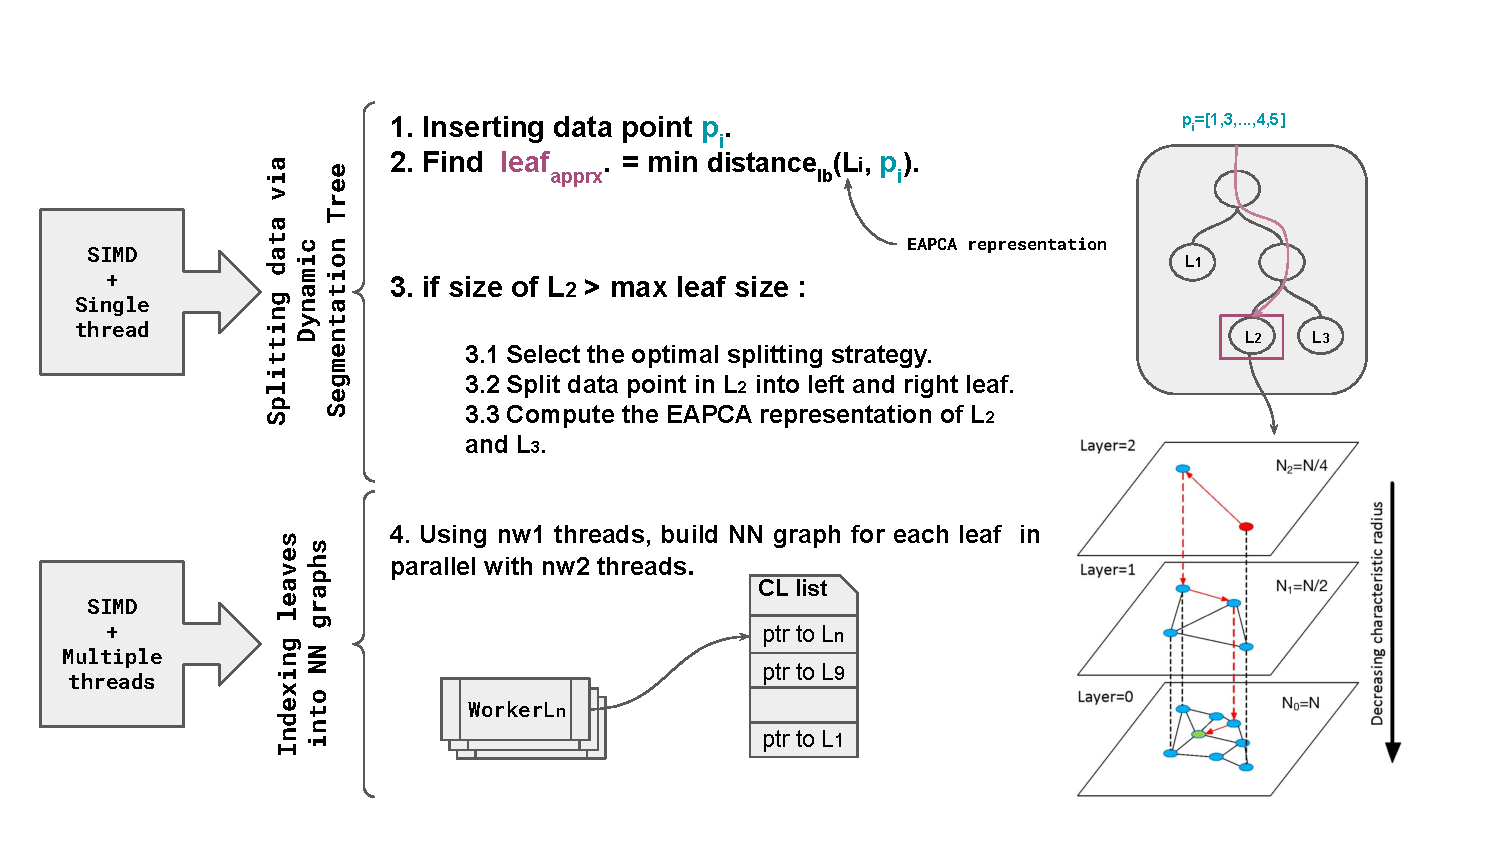
\includegraphics[width=0.90\textwidth] {../img/elpis/indexing_wf.pdf}
\caption{ELPIS Index Building Workflow}
\label{fig:hercules-index-building}
\end{figure}

ELPIS then proceeds with building an HNSW graph for each leaf in parallel. 
The main coordinator thread initializes ${n_1}$ leafCoordinator threads. 
Each leafCoordinator selects a leaf for which the graph was not built yet and creates ${n_2}$ leafWorker threads. 
Both the leafCoordinator and the leafWorkers contribute in building the graph within their corresponding leaf. 
Each one of them reads a vector from the dataset and inserts it into the graph.  
Once the graph has been built, the leafCoordinator materializes it into a separate file on disk and selects a new leaf to process. 
Index construction terminates once the graphs for all index leaves have been built.

\subsubsection{Query Answering}

Answering a query $V_Q$ with ELPIS proceeds in two major steps: (1) the Hercules tree is traversed to find $k$ initial best-so-far (bsf) neighbors to $V_Q$, which are then used to select a list of $l$ candidate leaves, i.e., clusters; and (2) a beam search is performed in parallel on the graph structures corresponding to the $l$ candidate leaves.

\begin{figure*}[tb]
\captionsetup{justification=centering}	
\begin{subfigure}{\textwidth}
\centering
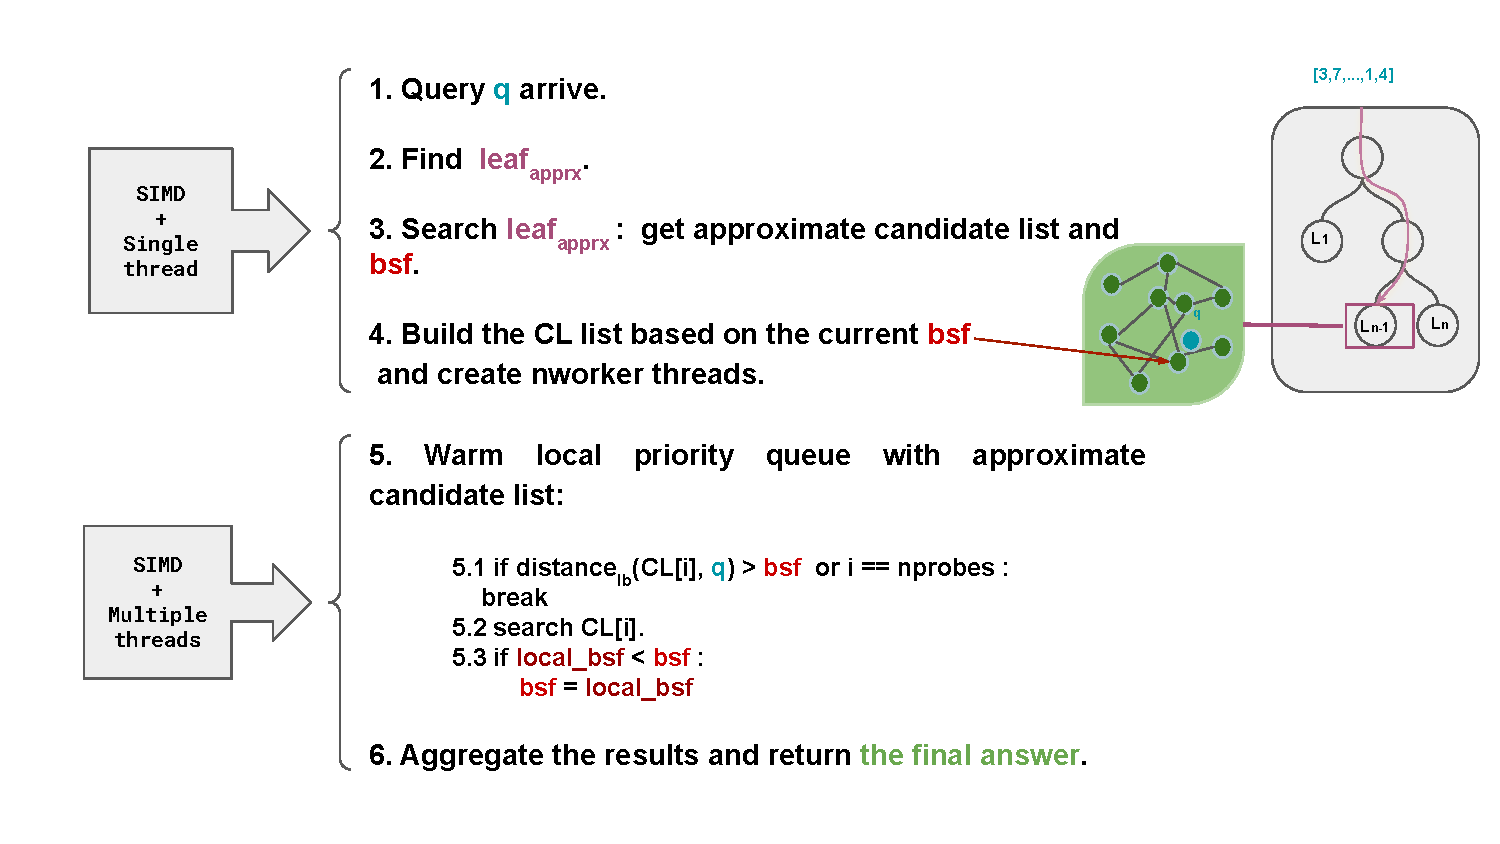
\includegraphics[width=0.90\textwidth] {../img/elpis/search_wf.pdf}
\end{subfigure}
\caption{Elpis query answering workflow}
\label{fig:Elpis-search}
\end{figure*}

During the first step, ELPIS traverses the Hercules tree, which is pre-loaded into memory, to find the leaf where $V_Q$ would have been inserted if it belonged to the dataset. Then, it performs a beam search on the HNSW graph corresponding to this leaf, returning the $k$ closest vectors to $V_Q$ as the first bsf answers. ELPIS resumes the traversal of the index tree using both the $k^{th}$ bsf answer and the EAPCA segmentation to prune nodes. The algorithm then returns, as candidate clusters, a list of $l$ leaves sorted in increasing order of their $LB_{EAPCA}$ distance to $V_Q$. 

In the second step, multiple threads process the candidate clusters in parallel, starting with the leaves that have the lowest $LB_{EAPCA}$ distances to $V_Q$. 
(Exploiting parallelism within the same graph is still an open problem and is beyond the scope of this paper, so each leaf graph is processed by only one thread, but the same thread can process multiple leaves, one at a time.) 
A thread processes a leaf by running a beam search on the corresponding HNSW graph and returning $k$ bsf answers. 
Each thread maintains a local priority queue which stores the $k$ bsf answers corresponding to the processed leaf and a local $k^{th}_{dist}$, the Euclidean distance between $V_Q$ and the $k^{th}$ bsf answer in the current leaf. 
The threads use a readers-writer lock to synchronize access to a global $k^{th}_{dist}$, the Euclidean distance between $V_Q$ and the $k^{th}$ bsf answer across all leaves. 
The global $k^{th}_{dist}$ bsf is updated every time a thread finds a better local $k^{th}_{dist}$ bsf answer. 
Once a thread finishes searching within a leaf, it uses its existing priority queue to warm up a new search on the next leaf with the lowest $LB_{EAPCA}$ to $V_Q$. 
Search terminates either after the $l$ candidate clusters are processed or once the $LB_{EAPCA}$ distances between $V_Q$ and the next leaf to be processed are larger than the $k^{th}_{dist}$. 
This is because (i) the $LB_{EAPCA}$ distance guarantees the lower-bounding property, i.e., the Euclidean distance between any two points in the original high-dimensional space is guaranteed to be larger than or equal to their $LB_{EAPCA}$ distance; and (ii) the list of candidate leaves is sorted in increasing order of $LB_{EAPCA}$. 
Once all threads terminate, ELPIS computes the final results: it aggregates the answers from all local priority queues and selects the $k$ answers with the smallest Euclidean distance to $V_Q$.

\section{Experimental Evaluation}
\label{sec:experiments}

In this section, we conduct a comprehensive experimental evaluation of ten state-of-the-art graph-based vector search methods, including ELPIS. We assess the indexing and query-answering performance of these methods on a variety of real and synthetic datasets. All artifacts are available in~\cite{url/GASS}.

\subsection{Framework}
\noindent{\bf Setup.} 
Methods were compiled with GCC 8.2.0 under Ubuntu Linux 20.04 (Rocky Linux 8.5 on HPC) using default compilation flags and optimization level 3. Experiments were conducted on an Intel Xeon Platinum 8276 server with 4 sockets, each with 28 cores and 1 thread per core.
The CPU cache configuration is: 32KB L1d, 32KB L1i, 1,024KB L2, and 39,424KB L3 cache. The server includes a 1.5TB RAM via 24x 64GiB DDR4 DIMMs.}

\noindent{\bf Algorithms.} We cover the following methods: ELPIS~\cite{elpis}, HNSW~\cite{hnsw}, NSG~\cite{nsg}, Vamana~\cite{vamana}, EFANNA~\cite{efanna}, HCNNG~\cite{hcnng}, DPG~\cite{dpg}, KGraph~\cite{kgraph}, NGT~\cite{ngt_library}, DPG~\cite{dpg}, and two versions of SPTAG~\cite{SPTAG4} (SPTAG-BKT and SPTAG-KDT, using BKT and K-D Trees, respectively). We also included LSHAPG~\cite{lshapg}, new technique not evaluated in the latest survey~\cite{graph-survey-vldb}. IEH~\cite{ieh} and FANNG~\cite{fanng} are excluded due to suboptimal performance~\cite{graph-survey-vldb, nsg}, and HVS~\cite{hvs} due to difficulties running the official implementation~\cite{hvsgithub}. We use the most efficient publicly available C/C++ implementations for each algorithm, leveraging multi-threading and SIMD vectorization to optimize performance.  We also carefully inspected all code bases and, as is common in the literature ~\cite{graph-survey-vldb, diskanncode, nsgcode,ssgcode,ngtcode,sptagcode}, disabled the optimizations that would lead to an unfair evaluation such as cache pre-warming in Vamana and L2-normalized Euclidean distance in NSG, EFANNA, and Vamana. Since all methods except ELPIS and HNSW use a single linear buffer as a priority queue, we modified the original implementations of these two algorithms (which used two max-heap priority queues)~\cite{url/Elpis,url/hnsw}. The modifications to each code base are documented in~\cite{url/GASS}. All algorithms were tuned to achieve a good accuracy/efficiency trade-off (Please refer to Appendix~\ref{appendix:parameters} for more details on the parameters tuning and choice) . 

\noindent{\bf Datasets.} 
We use seven real-world datasets from various domains, including deep network embeddings, computer vision, neuroscience, and seismology:  
(i) \emph{Deep}~\cite{url/data/deep1b} contains 1 billion 96-dimensional vectors extracted from the final layers of a convolutional neural network;  
(ii) \emph{Sift}~\cite{conf/icassp/jegou2011,url/data/sift} consists of 1 billion 128-dimensional SIFT vectors representing image feature descriptors;  
(iii) \emph{SALD}~\cite{url/data/eeg} provides neuroscience MRI data with 200 million 128-dimensional data series;  
(iv) \emph{Seismic}~\cite{url/data/seismic} contains 100 million 256-dimensional time series representing earthquake recordings from seismic stations worldwide;  
(v) \emph{Text-to-Image}~\cite{url/data/text2image} offers 1 billion 200-dimensional image embeddings from Se-ResNext-101 along with 50 million DSSM-embedded text queries for cross-modal retrieval under domain shifts;  
(vi) \emph{GIST}~\cite{gist} contains 1 million 960-dimensional vectors, using GIST descriptors~\cite{gistdesc} to capture spatial structure and color layout of images;  and
(vii) \emph{ImageNet1M}, a new dataset that we generated from the original ImageNet~\cite{imagenet}, producing embeddings of 1 million original vectors using the ResNet50 model~\cite{resnet}, with PCA applied to reduce dimensionality to 256. We select subsets of different sizes from the Sift, Deep, SALD and Seismic datasets, and we refer to each subset with the name of the dataset followed by the subset size in GBs (e.g., Deep25GB). 
We refer to the 1-million and 1-billion datasets with the 1M and 1B prefixes, respectively. 
To evaluate the methods on datasets with different distributions, we generate three random 25GB datasets RandPow0, % (uniform distribution~\cite{url/Elpis}), 
RandPow5 and RandPow50, each with 256 dimensions, following the power law distribution~\cite{powerlaw} using three power law exponents: 0 (uniform~\cite{url/power-law}), 5 and 50 (very skewed).
The power law distribution models many real world phenomena (including in economics, physics, biology, social networks, etc.). 
It is a relationship of type $Y= kX^a$, where $Y$ and $X$ are variables of interest, $a$ is the power law exponent and $k$ is a constant. 
The skewness of a dataset distribution increases with $a$. 
When $a = 0$, the dataset is evenly distributed.

\noindent{\bf Dataset Complexity.}
The complexity of the datasets in our experimental evaluation is assessed using Local Intrinsic Dimensionality (LID)~\cite{lid15,DBLP:journals/is/AumullerC21} and Local Relative Contrast (LRC)~\cite{rc,DBLP:journals/is/AumullerC21}. 
The LID and LRC for a query point \( x \) are defined as follows:

\noindent{\textbf{Local Intrinsic Dimensionality (LID)}} The LID of a query point \( x \) provides a local estimate of the dimensionality around \( x \) based on the distances to its nearest neighbors. Formally, LID is defined as:

\begin{equation}
    \text{LID}(x) = -\left(\frac{1}{k} \sum_{i=1}^{k} \log \frac{\text{dist}_i(x)}{\text{dist}_k(x)}\right)^{-1}
    \label{eq:lid}
\end{equation}

Where:
\begin{itemize}
    \item \( x \) is the query point.
    \item \( \text{dist}_i(x) \) is the distance from \( x \) to its \( i \)-th nearest neighbor.
    \item \( \text{dist}_k(x) \) is the distance from \( x \) to its \( k \)-th nearest neighbor.
    \item \( k \) is the number of nearest neighbors considered.
\end{itemize}

\noindent{\textbf{Local Relative Contrast (LRC)}} The LRC metric quantifies the contrast between the mean distance to the neighbors of a query point and the distance to the \( k \)-th nearest neighbor. LRC is defined as:

\begin{equation}
    \text{LRC}(x) = \frac{\text{dist}_{\text{mean}}(x)}{\text{dist}_k(x)}
    \label{eq:lrc}
\end{equation}

Where:
\begin{itemize}
    \item \( \text{dist}_{\text{mean}}(x) \) is the mean distance from \( x \) to its \( k \)-nearest neighbors.
    \item \( \text{dist}_k(x) \) is the distance from \( x \) to its \( k \)-th nearest neighbor.
\end{itemize}

Figure~\ref{fig:datacomp:rc} presents the boxplot results for RC and LID values, calculated with a subset of one million data points randomly sampled from each dataset and a $k$ equals to 100. On the y-axis, we have the LID or LRC values, providing a measure of dataset complexity, while the x-axis enumerates the names of the datasets under investigation. High LRC in a dataset corresponds to distinctive data points, potentially marking boundaries or outliers, which could influence the stability and accuracy of k-NN results, whereas low LRC indicates homogeneous regions, leading to more consistent k-NN outcomes. 
High LID reveals complex, high-dimensional local structures, possibly complicating k-NN searches due to the “curse of dimensionality,” while low LID indicates simpler, low-dimensional areas, enhancing the efficiency and precision of k-NN searches. 
LID represents the intrinsic dimensionality of the data (and can be significantly lower than the original dimensionality of the data space): the lower the LID, the easier the search is.

\begin{figure}[tb]
    \centering
    \begin{subfigure}{0.48\columnwidth}
    \centering
			\captionsetup{justification=centering}	
        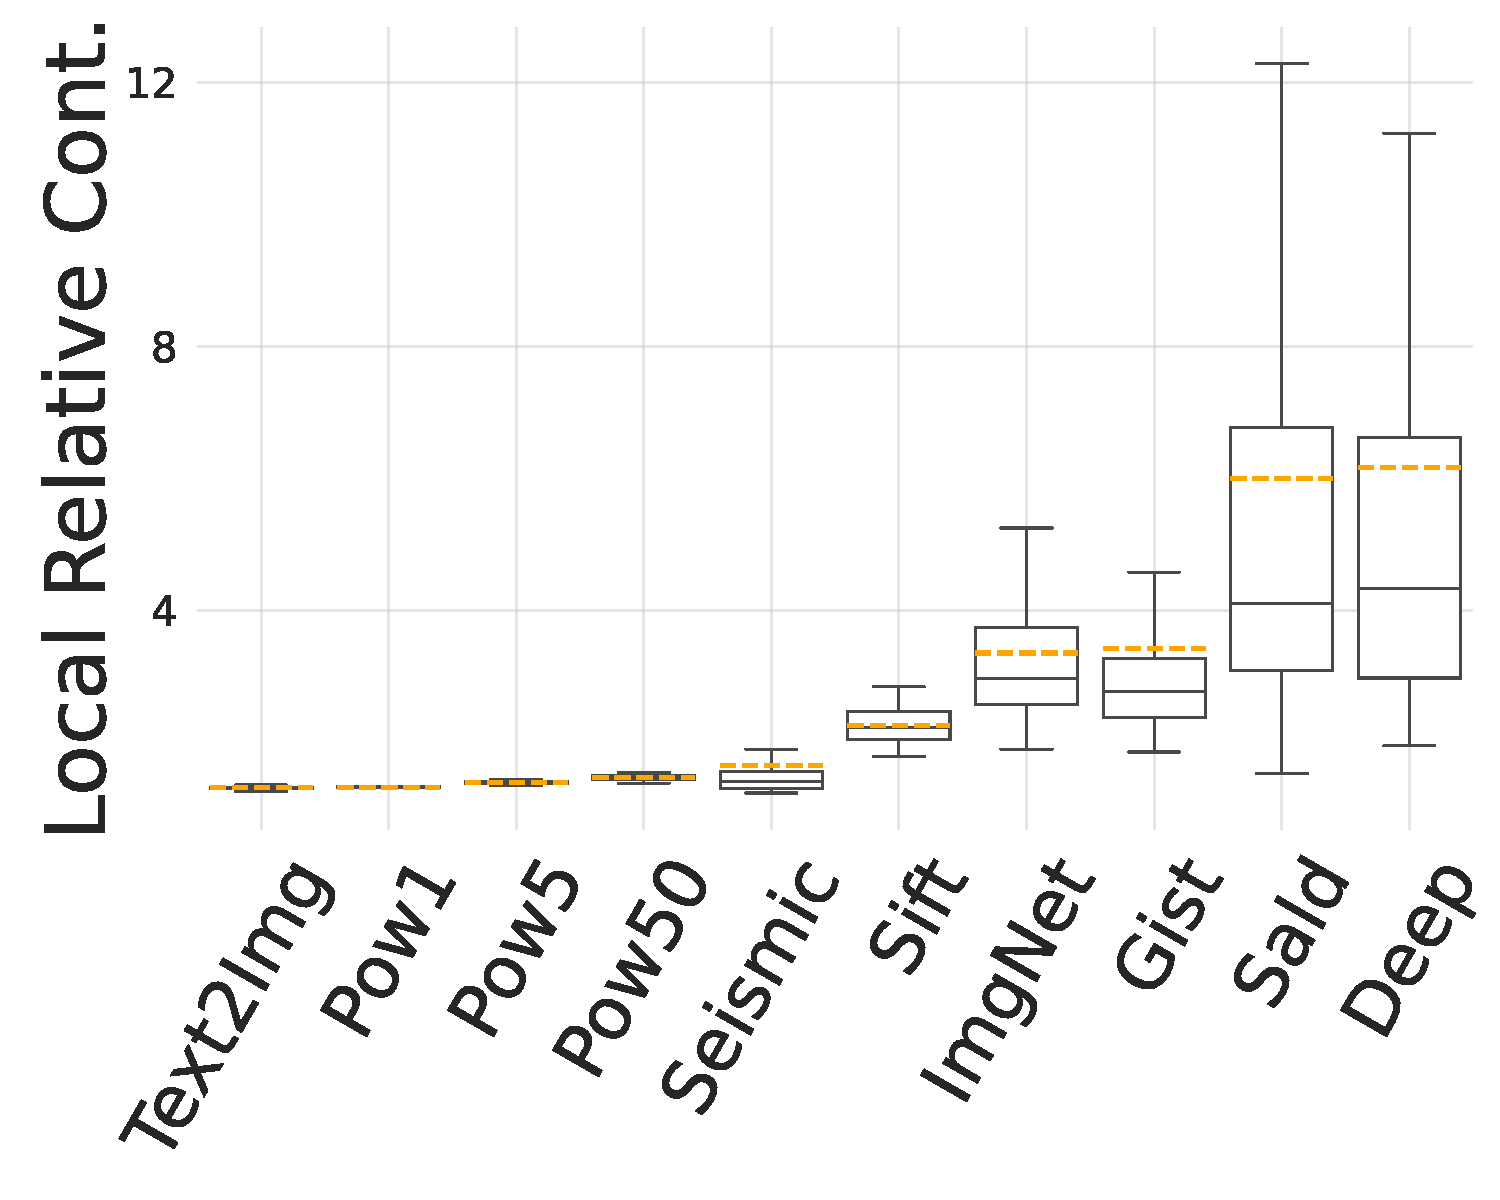
\includegraphics[width=\columnwidth]{../img/Experiments/data/query_rc_plot.pdf}
        \caption{Local Relative Contrast}
        \label{fig:datacomp:rc}
    \end{subfigure}
    \begin{subfigure}{0.499\columnwidth}
    \centering
			\captionsetup{justification=centering}	
        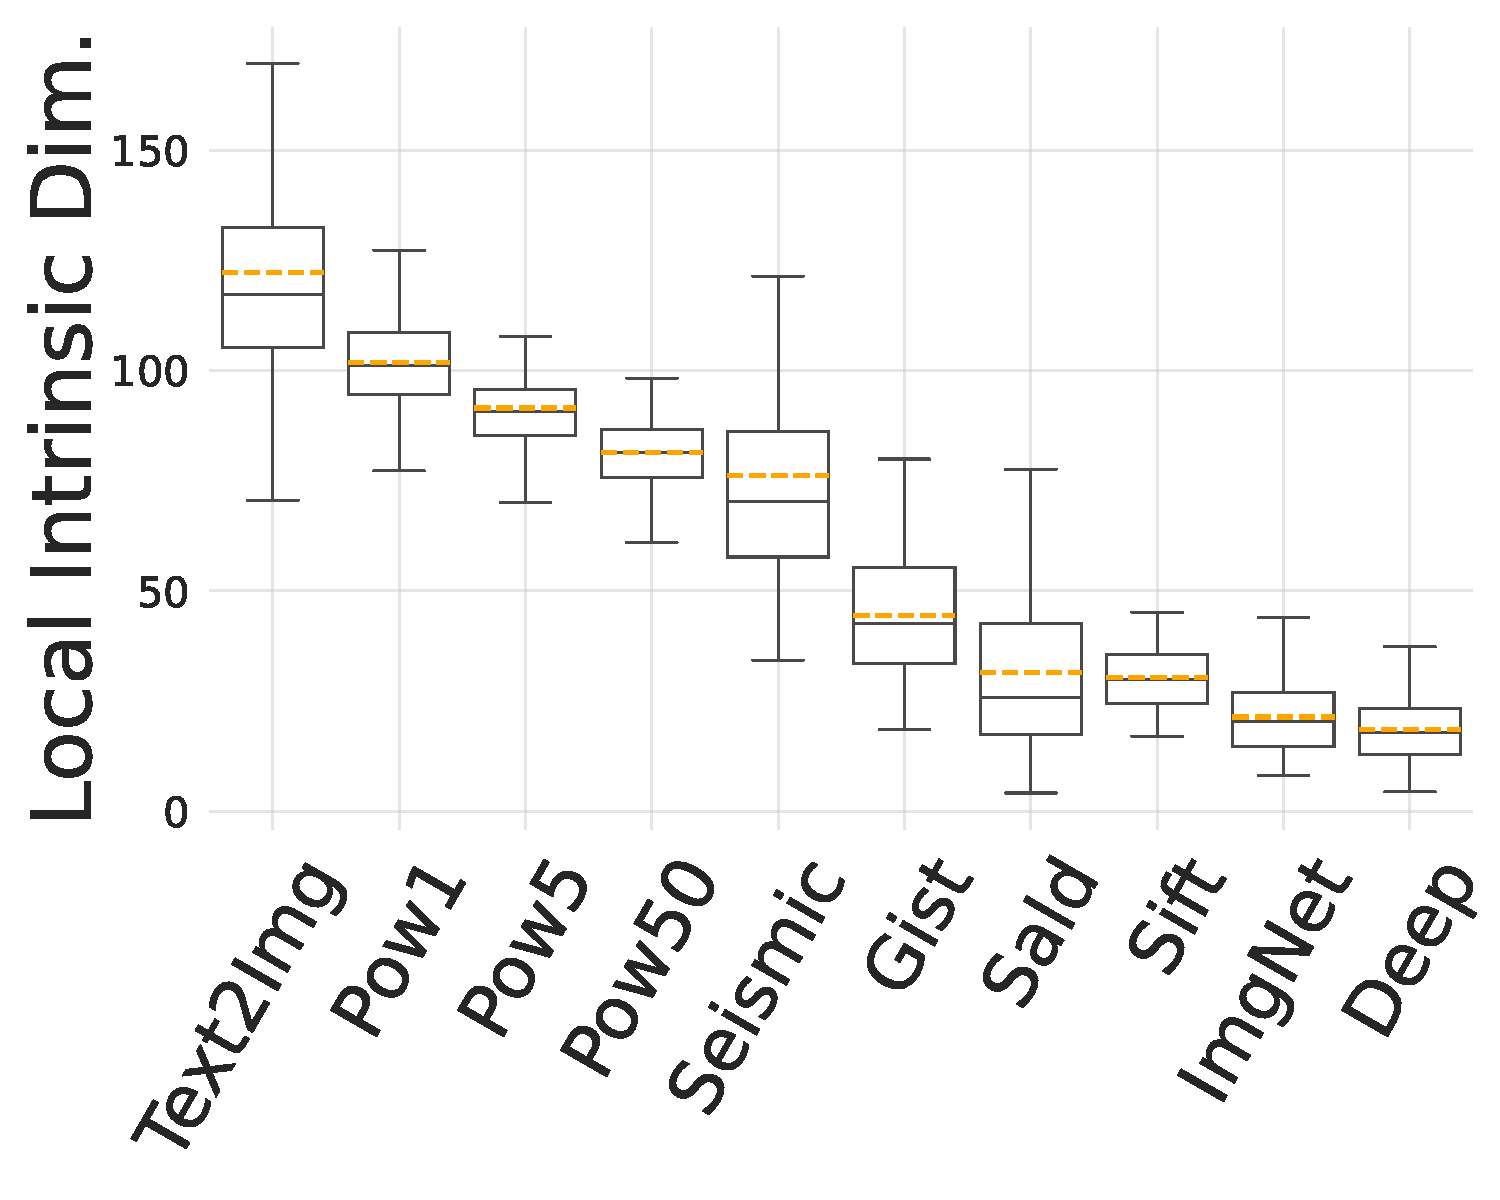
\includegraphics[width=\columnwidth]{../img/Experiments/data/query_lid_plot.pdf}
        \caption{Local Intrinsic Dimensionality}
        \label{fig:datacomp:lid}
    \end{subfigure}
    \caption{Dataset complexity}
    \label{fig:datacomp}
\end{figure}

Note that the orange horizontal line in Figure~\ref{fig:datacomp:rc} denotes the mean LRC, which corresponds to the Relative Contrast (RC)~\cite{DBLP:journals/is/AumullerC21} of the dataset. The Pow0, Pow5, Pow50, and Seismic datasets have the highest LID and lowest LRC values, indicating that they are challenging datasets for vector search~\cite{DBLP:journals/is/AumullerC21}.

The random datasets we generated are highly clustered and high-dimensional, reflecting the same difficulties for k-NN methods as the Text-to-image and Seismic datasets, and to a lesser extent, the SALD dataset. Meanwhile, Imagenet, Sift and Deep are the easiest datasets in our workload to query, with the lowest LID and highest LRC values. In the results section, we will remark how graph-based ng-approximate similarity search methods face high difficulties in achieving high accuracy for query answering in datasets with high LID and low LRC, and perform well when dealing with low LID and high LRC datasets.

\noindent{\bf Queries.}  Query sets include 100 vectors processed sequentially, not in batches, mimicking a real-world scenario where queries are unpredictable~\cite{itsawreport,DBLP:conf/edbt/GogolouTPB19,conf/sigmod/gogolou20}. Results with 1 million queries are extrapolated from 100 query sets. For Deep, Sift, GIST, and Text-to-Image, queries are randomly sampled from available query workloads. For SALD, ImageNet, and Seismic, 100 queries are randomly selected from the datasets and excluded from the index-building phase.
For hardness experiments, we use Deep query vectors of varying complexity, denoted as a percentage ranging from 1\% to 10\%. These vectors were obtained by adding Gaussian noise (\(\mu = 0\), \(\sigma^2\) ranging from 0.01 to 0.1) to randomly choose dataset vectors, with the percentage reflecting the \(\sigma^2\) value~\cite{johannesjoural2018}.
The 100-query workloads for the power law distribution datasets are generated following the same distributions using different seeds. % as its respective dataset. 
Unless otherwise stated, all experiments were conducted with 10-NN queries per the standard in the community~\cite{neurips-2021-ann-competition,url/Elpis,ann-benchmark-journal}.
We use 100-NN queries to evaluate dataset complexity because a higher k improves the estimation of LID and LRC (Eqs. 5.1-5.2).
\\
\noindent{\textbf{Accuracy Measures}} The accuracy of a $k$-NN query \( S_Q \) is evaluated using the \textit{Recall} metric~\cite{Recall}. Recall measures the proportion of true nearest neighbors that are correctly returned by the query. It is formally defined as:

\begin{equation}
    \text{Recall}(S_Q) = \frac{\# \text{true neighbors returned by } Q}{k}
    \label{eq:recall}
\end{equation}

Where:
\begin{itemize}
    \item \( S_Q \) is the set of neighbors returned by the query \( Q \).
    \item \( k \) is the number of true nearest neighbors.
\end{itemize}

The reported recall represents the average recall across all queries in the query workload.



\subsubsection{Choosing the Clustering Technique} 


\begin{figure}[tb] 
	\captionsetup{justification=centering}
	\centering
	\begin{subfigure}{\columnwidth}
 \centering
		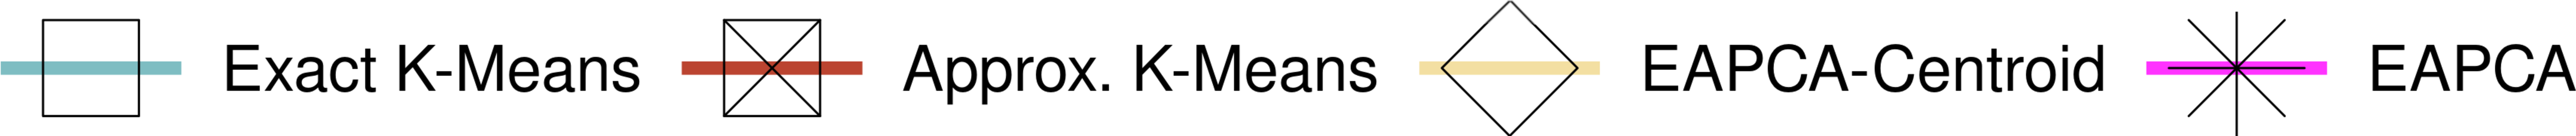
\includegraphics[width=0.7\columnwidth]{../img/elpis/ElpisvsKmeans/legend.pdf}
	\end{subfigure}	
	\begin{subfigure}{\sfig\columnwidth}
		\captionsetup{justification=centering}
		\centering
		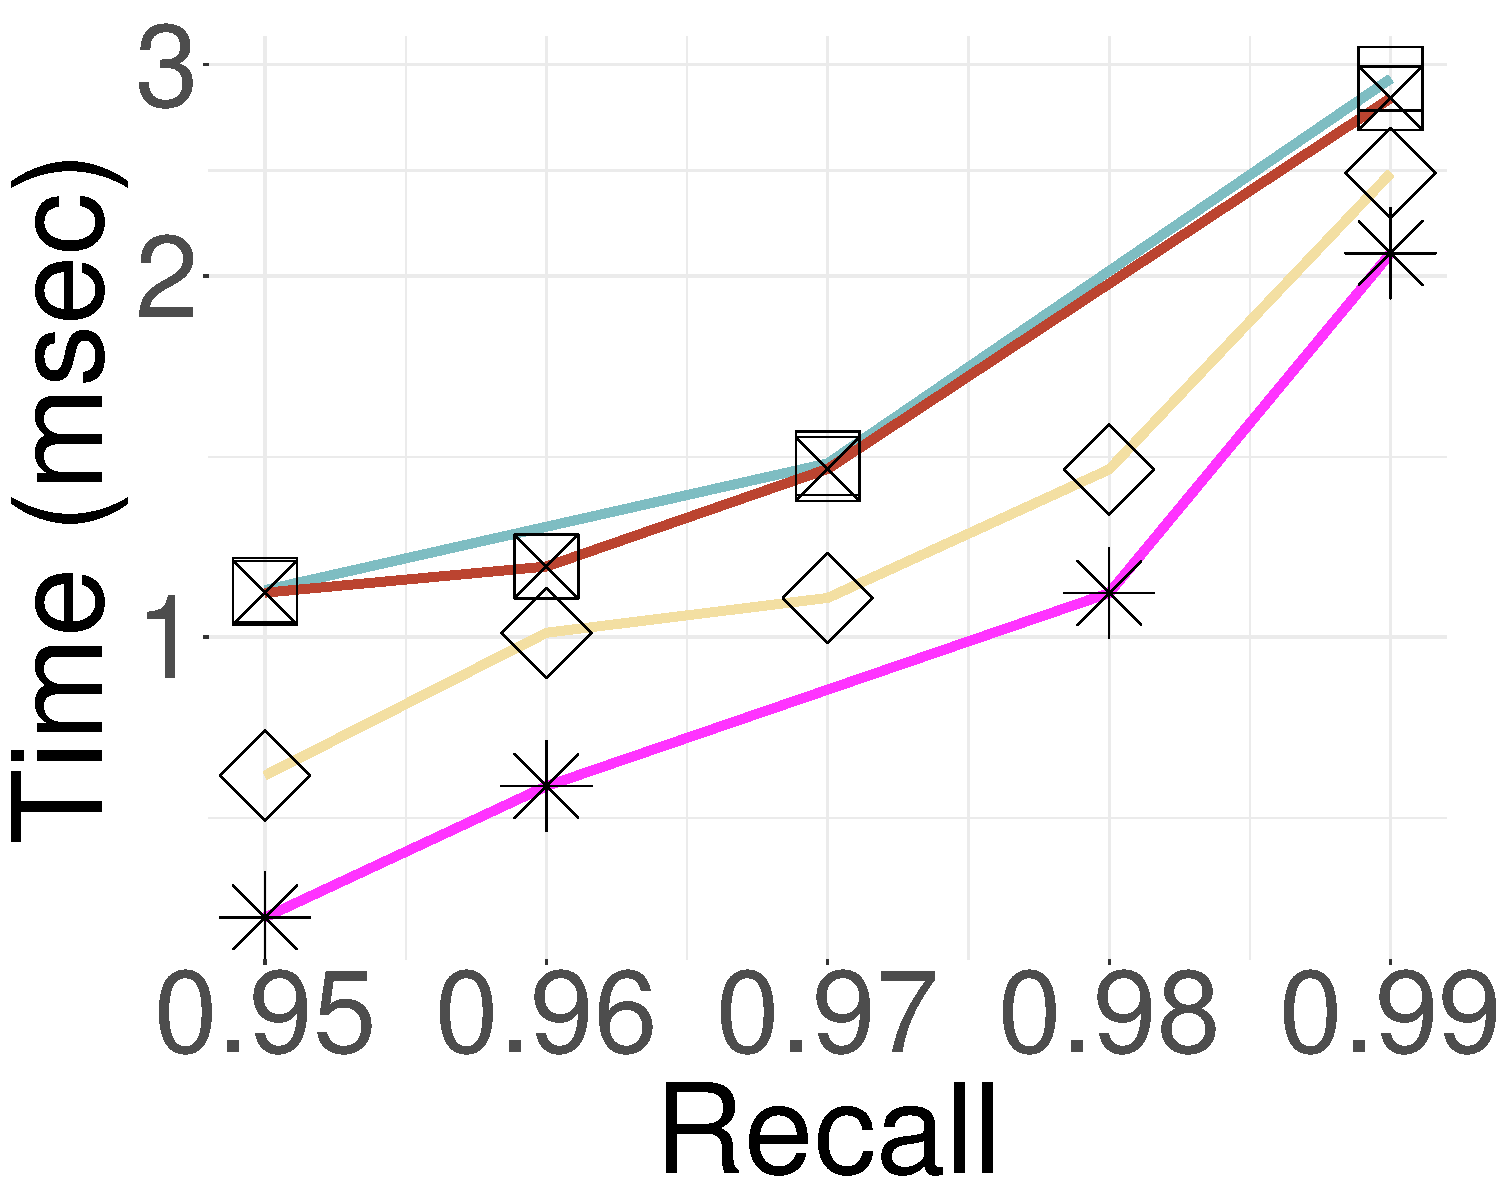
\includegraphics[width=\columnwidth]{../img/elpis/ElpisvsKmeans/qrstime.pdf}      
		\caption{Avg. query time} 
		\label{fig:elpis_kmeans:proc}
	\end{subfigure}	
 \hspace{0.4cm}
	\begin{subfigure}{\sfig\columnwidth}
		\captionsetup{justification=centering}
		\centering
		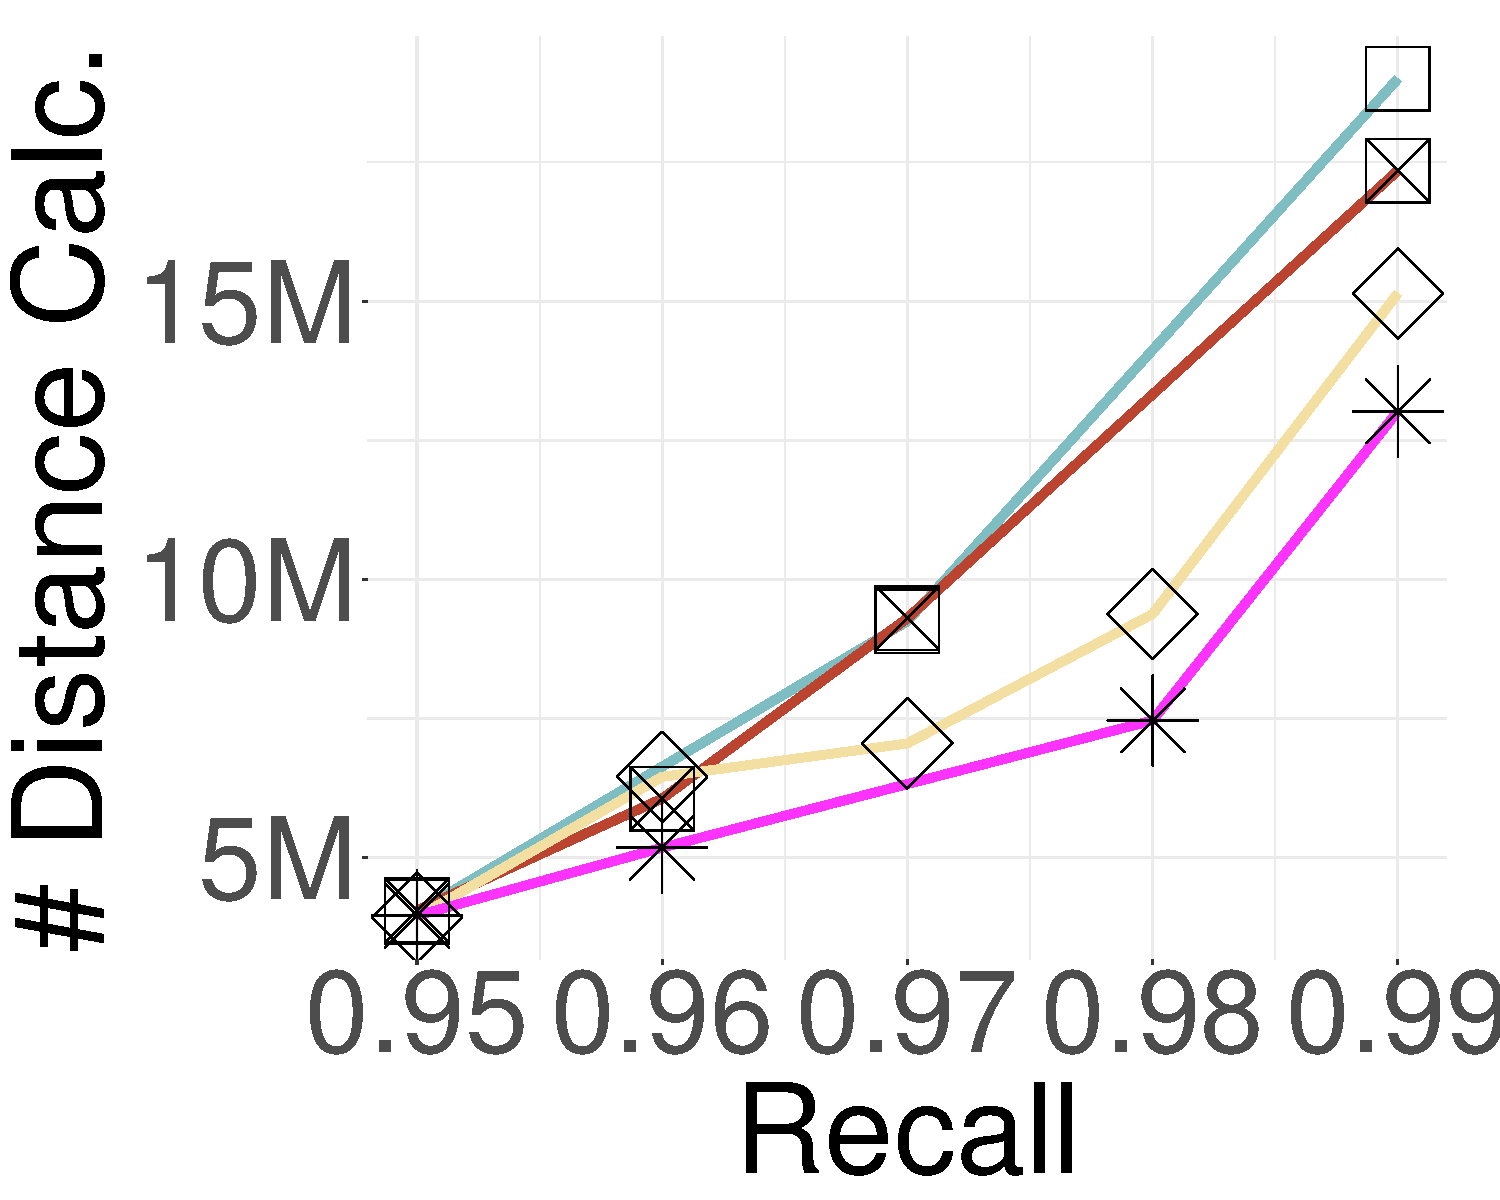
\includegraphics[width=\columnwidth]{../img/elpis/ElpisvsKmeans/qrsdc.pdf}                                                        
		\caption{Num. Dcs} 
		\label{fig:elpis_kmeans:distances}
	\end{subfigure}		


	\begin{subfigure}{\sfig\columnwidth}
		\captionsetup{justification=centering}
		\centering
		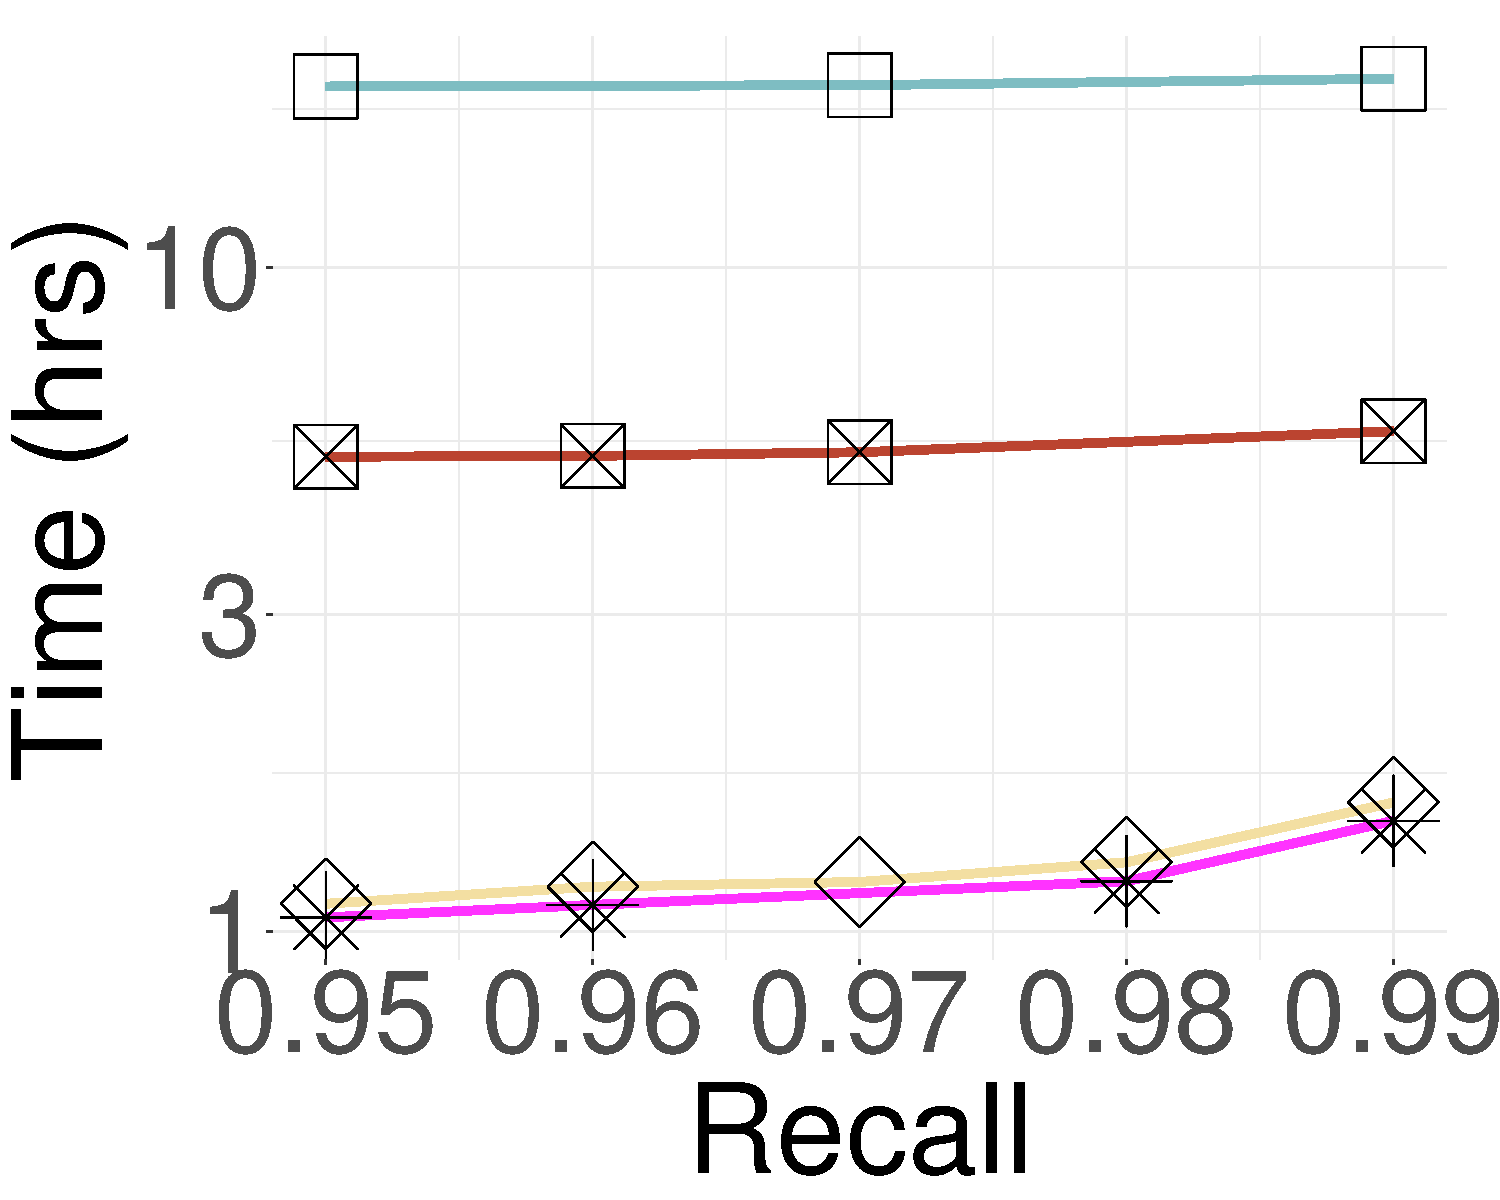
\includegraphics[width=\columnwidth]{../img/elpis/ElpisvsKmeans/idxqrs.pdf}                                             \caption{Idx+1M queries} 
		\label{fig:elpis_kmeans:idxproc}
	\end{subfigure}
  \hspace{0.4cm}
	\begin{subfigure}{\sfig\columnwidth}
		\captionsetup{justification=centering}
		\centering
		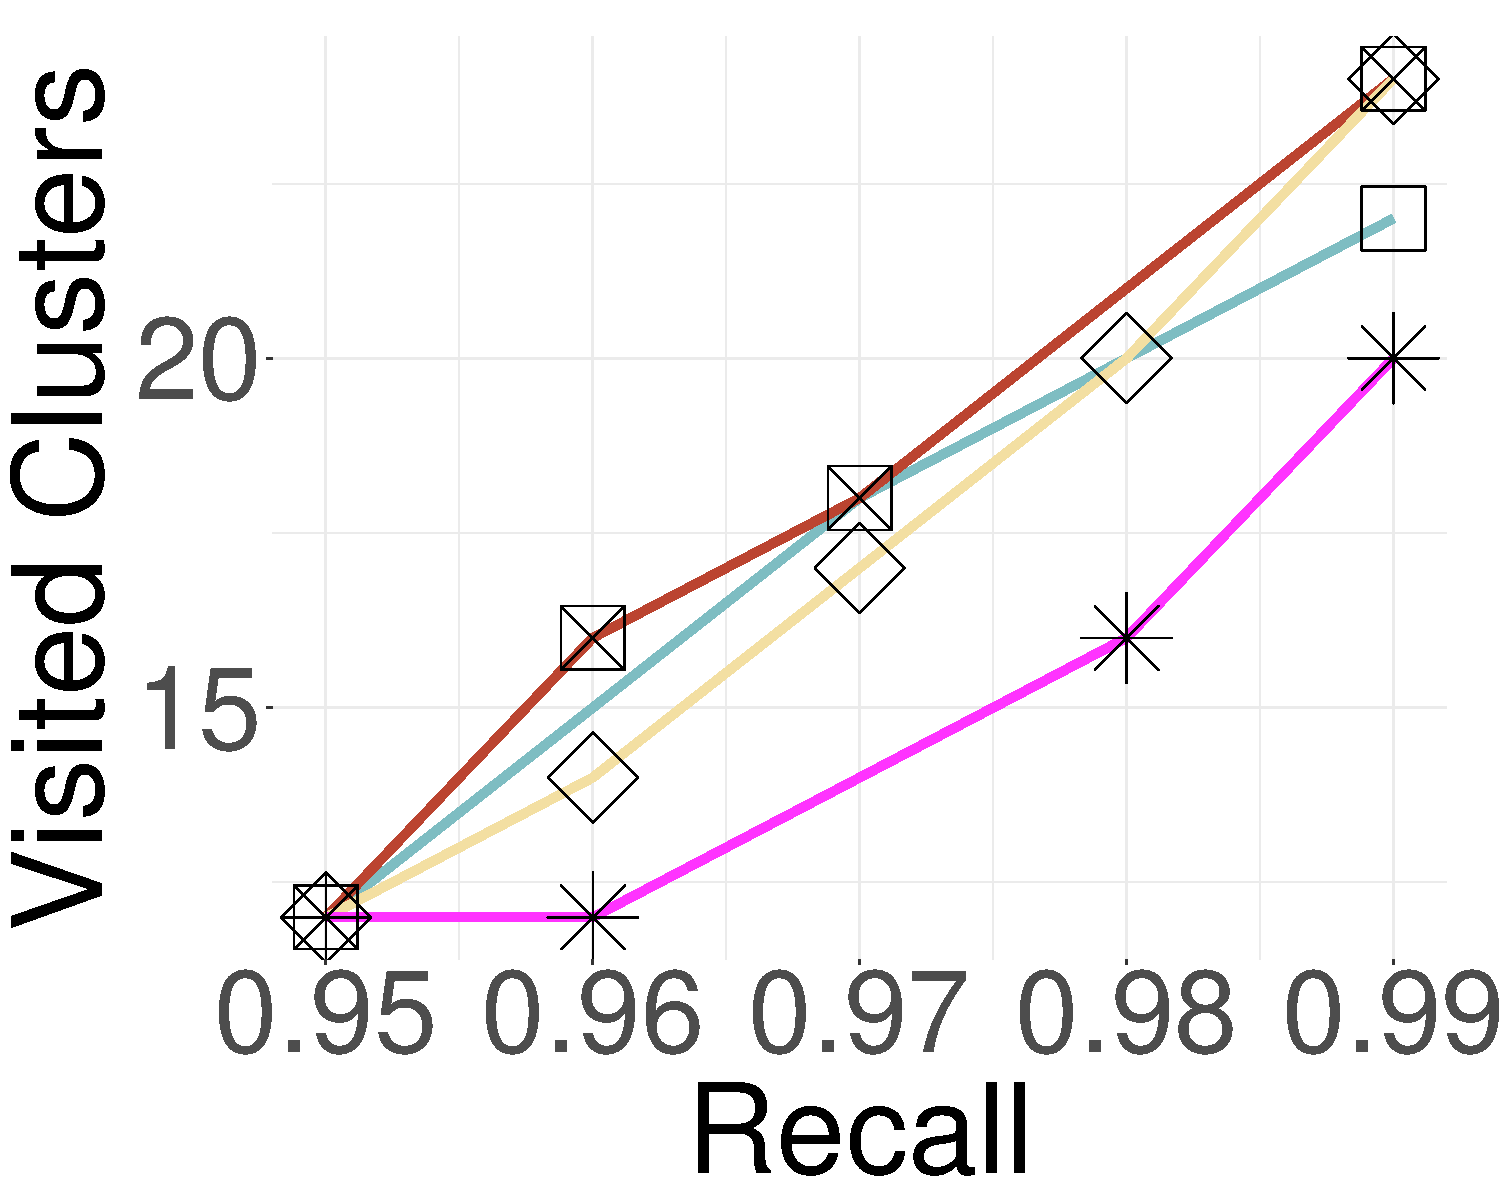
\includegraphics[width=\columnwidth]{../img/elpis/ElpisvsKmeans/qrsnprobes.pdf}                                                             
		\caption{Visited clusters} 
		\label{fig:elpis_kmeans:clusters}
	\end{subfigure}	
	\vspace*{-0.2cm}
	\caption{K-means vs EAPCA (Deep25GB)  } 
	\label{fig:elpis_kmeans}
\end{figure}


We evaluate three different clustering techniques: EAPCA-based clustering, exact K-means and approximate K-means. 
Exact K-means is the K-means algorithm in~\cite{kmeanshistory} that continues iterating until all centroids stabilize. 
Approximate K-means refers to a modified version of the exact K-means which stops execution after a certain number of iterations (user-defined). 
We evaluate different numbers of iterations and choose the one that leads to the same accuracy as the exact K-means. 
For a fair comparison, we use the number of clusters produced by the EAPCA clustering (which is not known in advanced, but determined adaptively) as the number of clusters in both K-means algorithms. 
Note that the points allocated to each cluster may be different across clustering techniques. 
The set of clusters produced by each technique is then fed to the same algorithm, which builds in parallel an HNSW graph in each cluster. 
In the case of ELPIS, the clusters correspond to the EAPCA-based Hercules tree leaves, and the entire tree represents the index. 
For the other techniques, the index consists only of the set of clusters. 
The query answering algorithm within each cluster is the same across techniques, but the pruning of clusters depends on the clustering approach: in the case of EAPCA-based clustering, we search clusters in ascending order of $LB_{EAPCA}$ (lower bounding distance between the query and the EAPCA representations of the clusters), and we prune clusters using both $LB_{EAPCA}$ and $k^{th}_{dist}$, the distance between the query and the current $k^{th}$ bsf answer, obtained by traversing the Hercules tree. 
Both exact and approximate K-means prune clusters based on the distance between the query and the cluster centroids. 
We also evaluate the pruning of the clusters using EAPCA-based clustering with centroid-based pruning (EAPCA-Centroid). EAPCA-Centroid uses the same clusters obtained by the EAPCA clustering, but prunes clusters using the distances to the cluster centroids (instead of $LB_{EAPCA}$ and $k^{th}_{dist}$).


Figure~\ref{fig:elpis_kmeans} summarizes the results of this experiment on the Deep25GB dataset. 
To ensure a fair comparison between EAPCA and K-means, we use the same number of clusters. Since in EAPCA, this number is found adaptively and cannot be enforced, we use the number of leaves that result from building the EAPCA tree as the number of clusters for the K-means algorithms (in the case of Deep25GB, this number is 26). 
The exact K-means algorithm requires 551 iterations to converge, while approximate K-means requires 40 iterations to reach the accuracy levels of exact K-means.
We observe that on average  for a given query, ELPIS delivers the same accuracy as previous methods up to 1.5x faster (Figs.~\ref{fig:elpis_kmeans:proc}-~\ref{fig:elpis_kmeans:distances}). 
At the same time, it builds the index and answers 1 million queries 5x-15x faster than competitors  (Fig.~\ref{fig:elpis_kmeans:idxproc}). 
We report that ELPIS builds its index 4x and 60x faster than the solutions using approximate and exact K-means, respectively, even though they are building the same number of clusters. This is because both exact and approximate K-means spend a significant amount of time to find the centroids and populate them with vectors, whereas ELPIS uses the efficient index building algorithm of Hercules.  
We can see in Figure~\ref{fig:elpis_kmeans:clusters} that the EAPCA clustering, used by ELPIS, achieves the same recall as EAPCA-Centroid by visiting a smaller number of clusters. 
Since they both use the exact same clusters and query algorithm within each cluster, this means that EAPCA prunes the clusters better than EAPCA-Centroid. 
For instance, EAPCA-Centroid needs to visit 20 clusters whereas EAPCA only needs to visit 16. 
Besides, by visiting the same number of clusters, EAPCA can reach a higher recall than EAPCA-Centroid, because it more intelligently selects the most promising clusters to search. 
\subsubsection{Choosing the Graph Structure Within Each Cluster}
In this experiment, we evaluate different state-of-the-art graph structures to choose the best performing one. We divide a dataset into several clusters using the EAPCA dynamic segmentation, then evaluate the indexing and query performance of different types of graphs within the clusters (ELPIS-H using HNSW; ELPIS-N and ELPIS-V using NSG and VAMANA respectively), and compare against the performance of the original graphs. Figure~\ref{fig:elpis:design:graph-type} demonstrates that using HNSW within the clusters leads to the best performance compared to using NSG or VAMANA, in both indexing and query answering.

\begin{figure}[tb]
	\captionsetup{justification=centering}
	\centering	
	\begin{minipage}{\columnwidth}
		\begin{subfigure}{\textwidth}
			\captionsetup{justification=centering}	
			\centering
			
\includegraphics[width=0.8\columnwidth]{../img/elpis/Idx/legend.pdf} 
			\label{fig:idx:time:comParIS+on:Hercules:ParIS+:andromache:coldcache}
		\end{subfigure}\\
		\vspace{-.4in}
	\end{minipage}
			
	\begin{minipage}{0.037\textwidth}
		\captionsetup{justification=centering}
		\captionsetup[subfigure]{justification=centering}
		\begin{subfigure}{\textwidth}		
		
\includegraphics[width=\columnwidth]{../img/Experiments/timeh.pdf}
	\vspace{.5in}	
  \end{subfigure}
	\end{minipage}
	\begin{minipage}{0.27\columnwidth}
	\vspace{0.18in}				
		\begin{subfigure}{\columnwidth}
			\captionsetup{justification=centering}	
			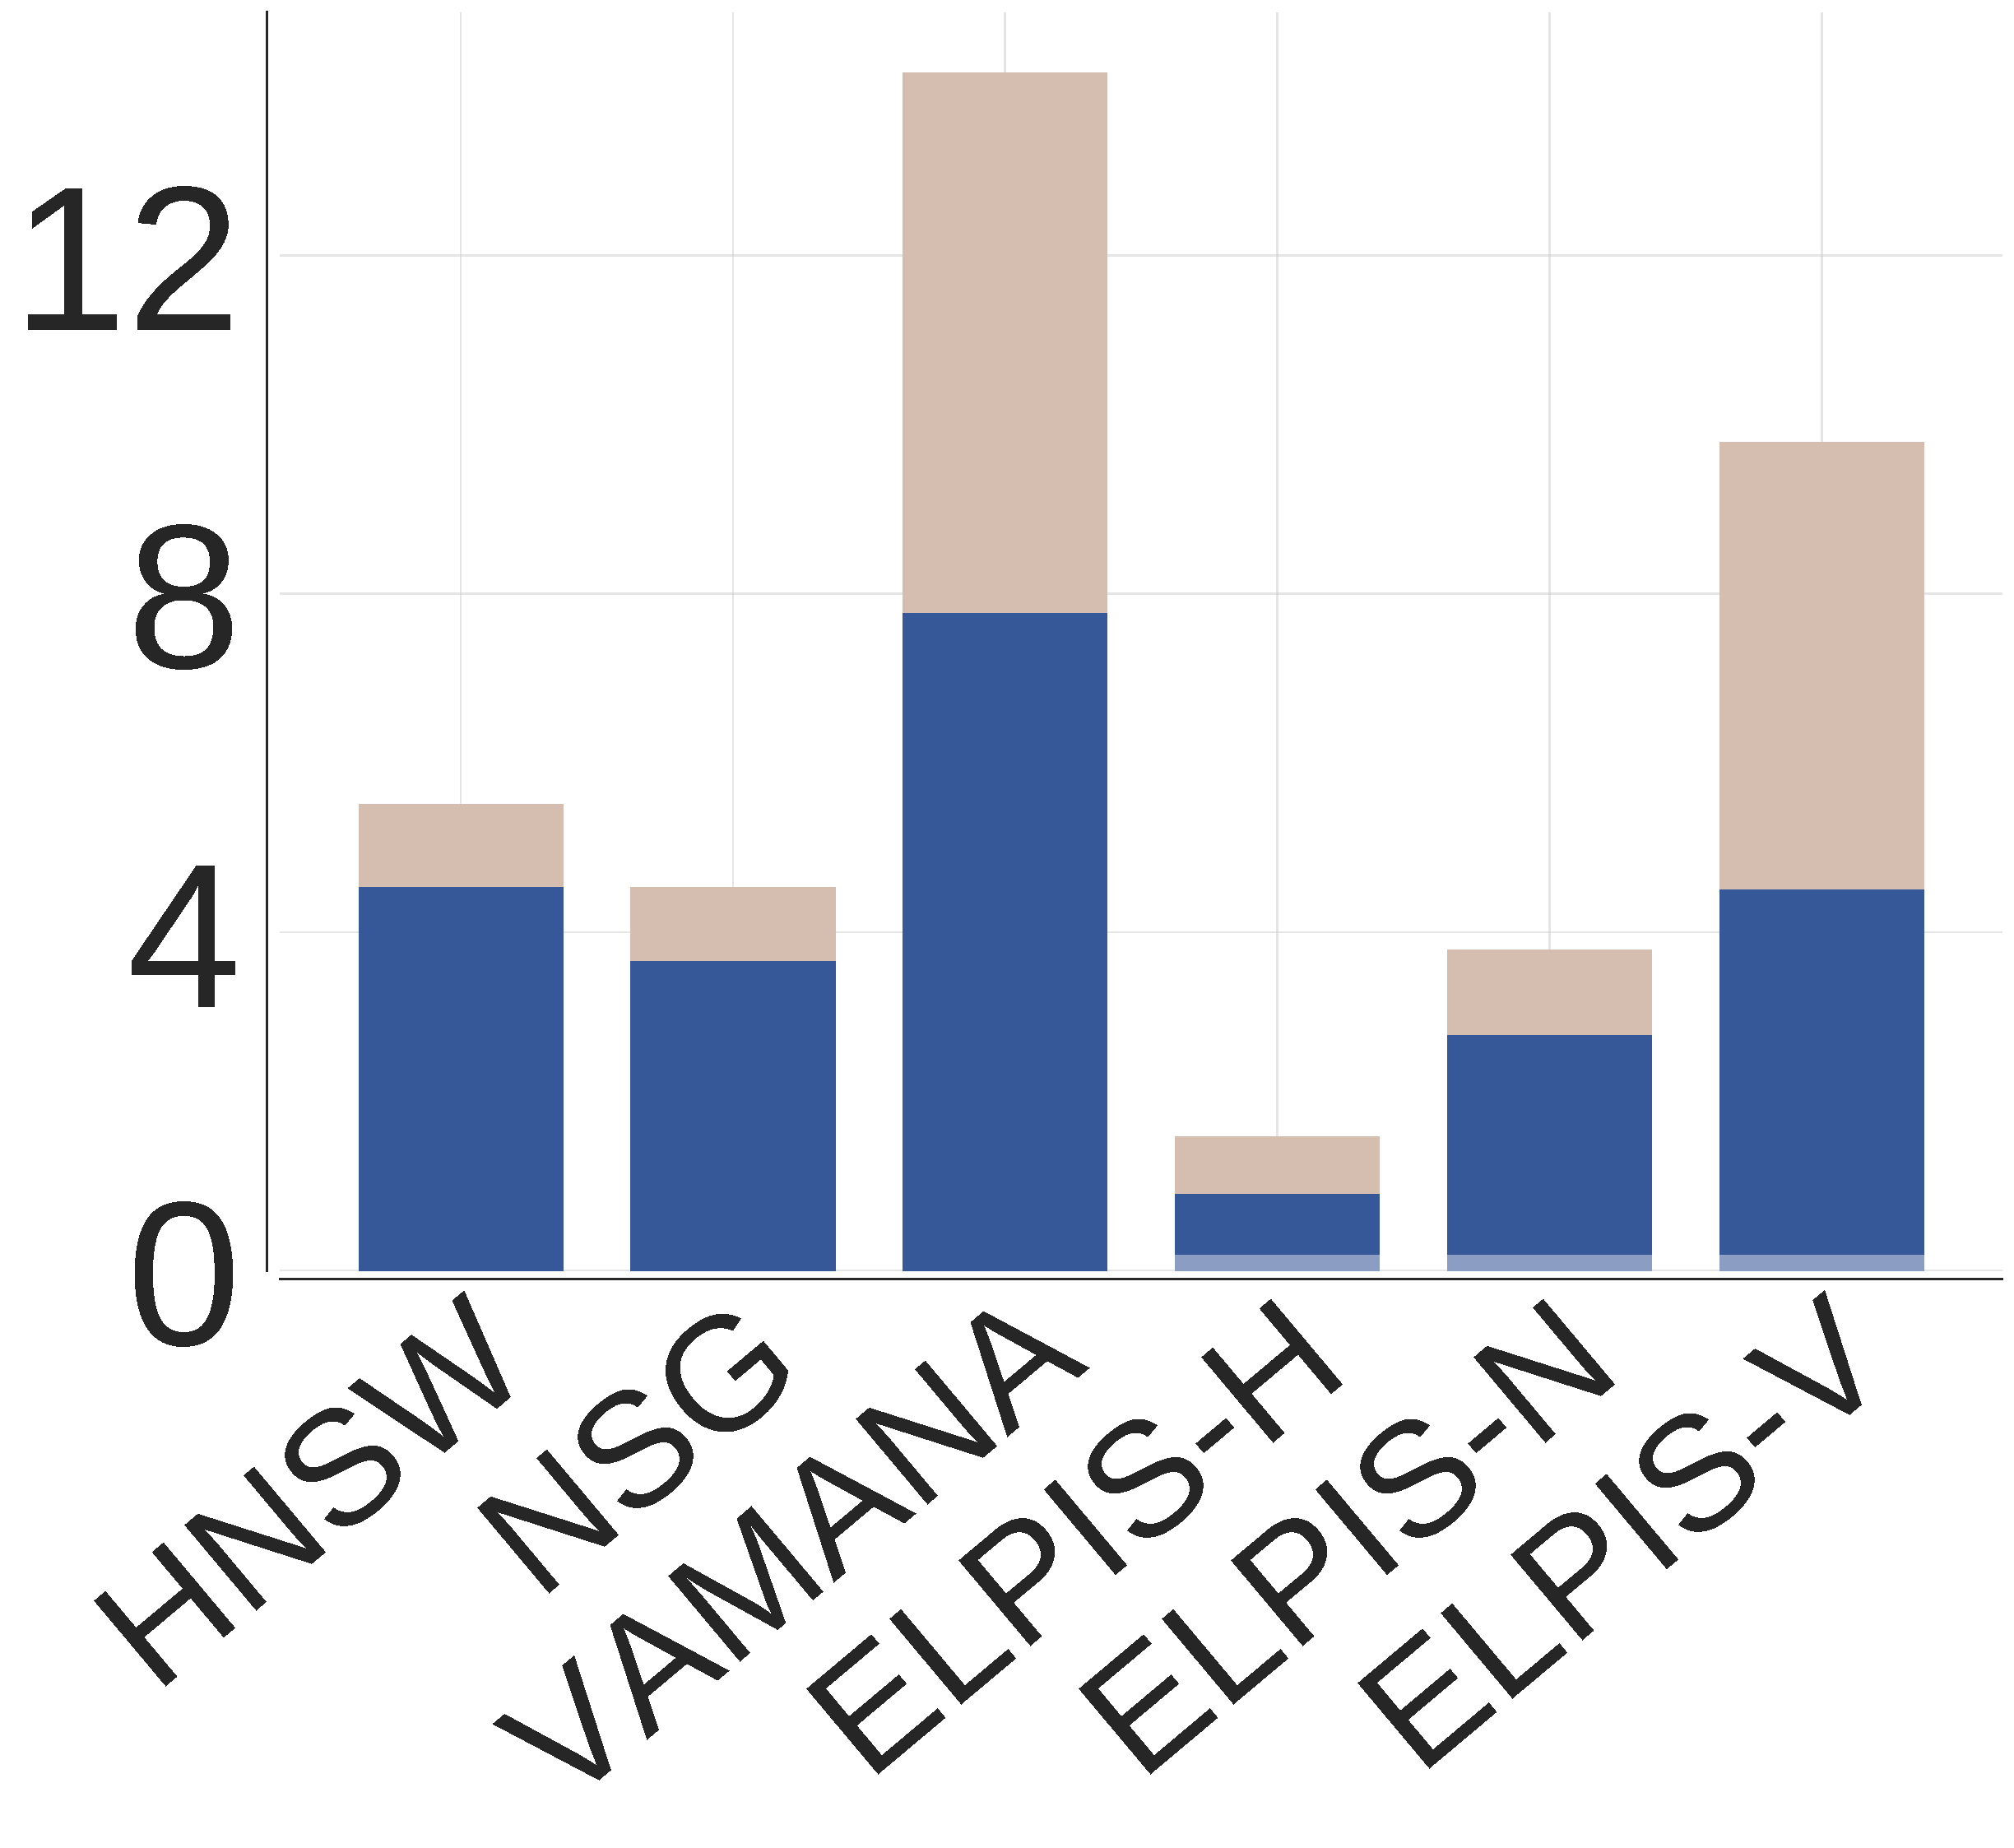
\includegraphics[width=\columnwidth]{../img/elpis/Idx/25_idx_comp.pdf} 
		\end{subfigure}	
	\vspace{-0.27in}
		\caption{{Varying graph structures (Deep25GB)}}
		\label{fig:elpis:design:graph-type}
	\end{minipage}	
	\begin{minipage}{0.295\columnwidth}
		\begin{subfigure}{\columnwidth}
			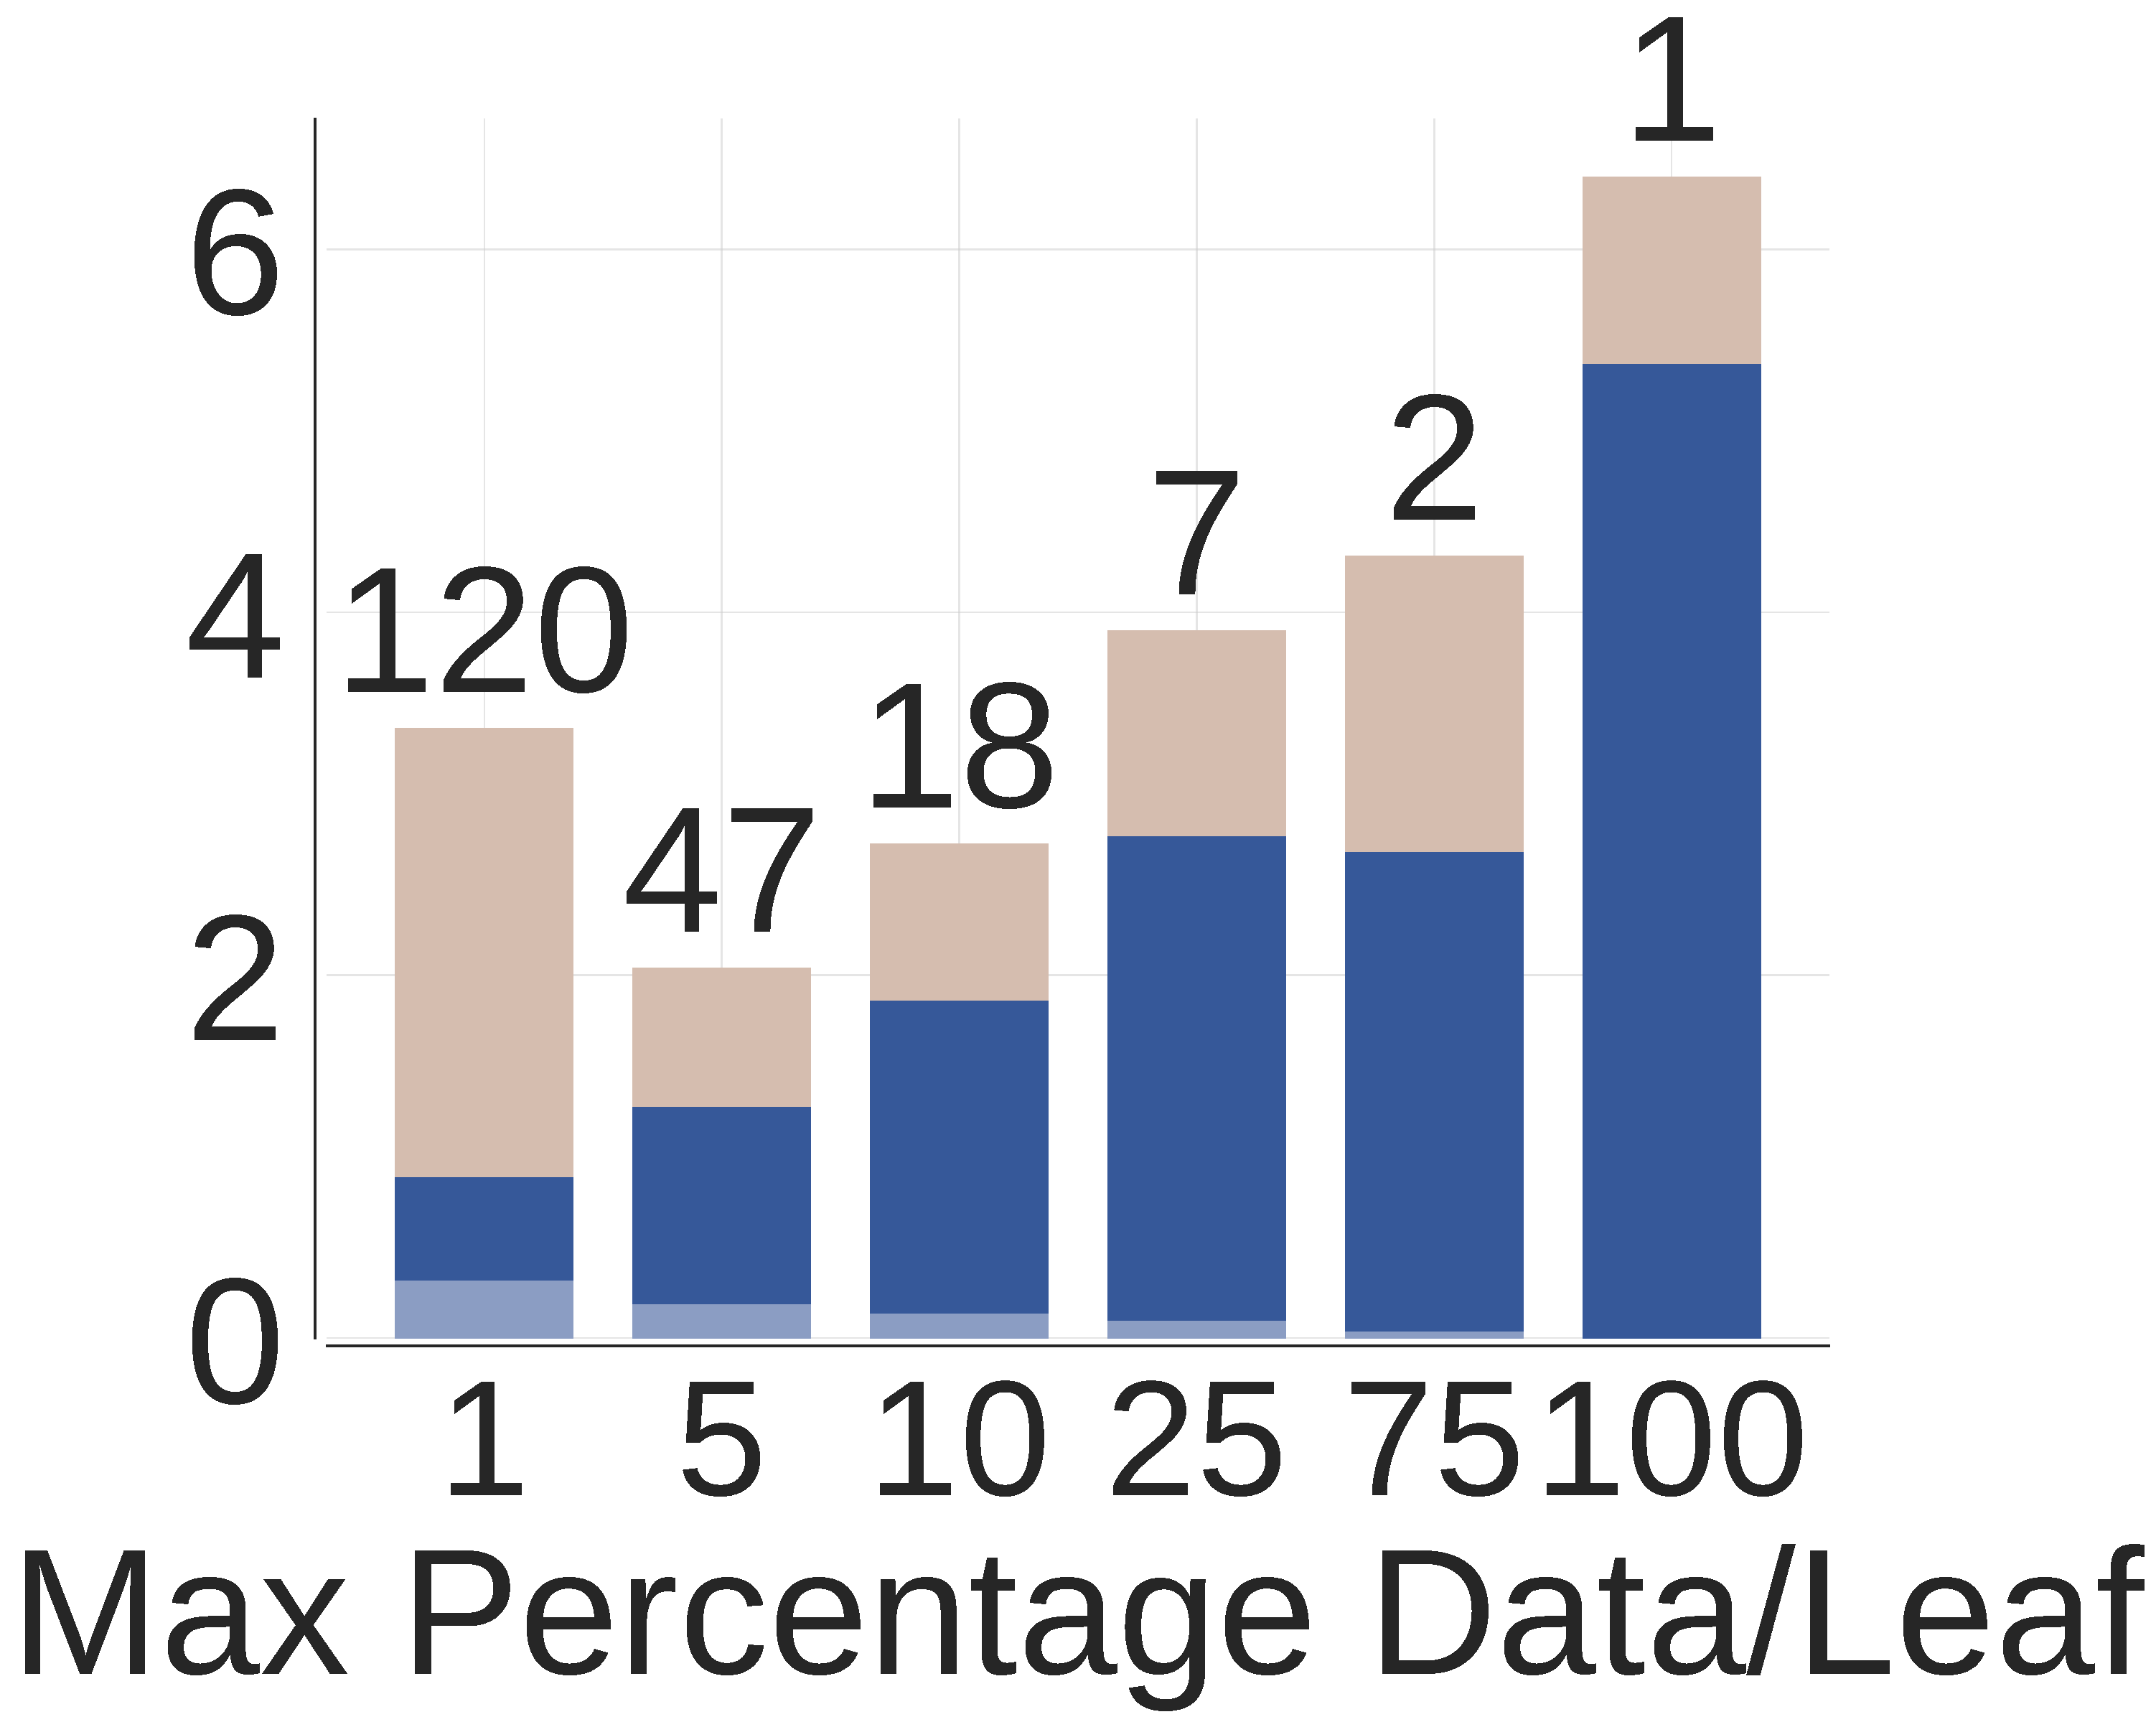
\includegraphics[width=\columnwidth]{../img/elpis/Idx/25_dpl_comp.pdf} 
		\end{subfigure} 
		\caption{{Varying cluster sizes (Deep25GB)}}
		\label{fig:elpis:design:cluster-size}
	\end{minipage}	
	\begin{minipage}{0.34\columnwidth}				
		\vspace{.05in}
		\begin{subfigure}{\columnwidth}
		\captionsetup{justification=centering}	
			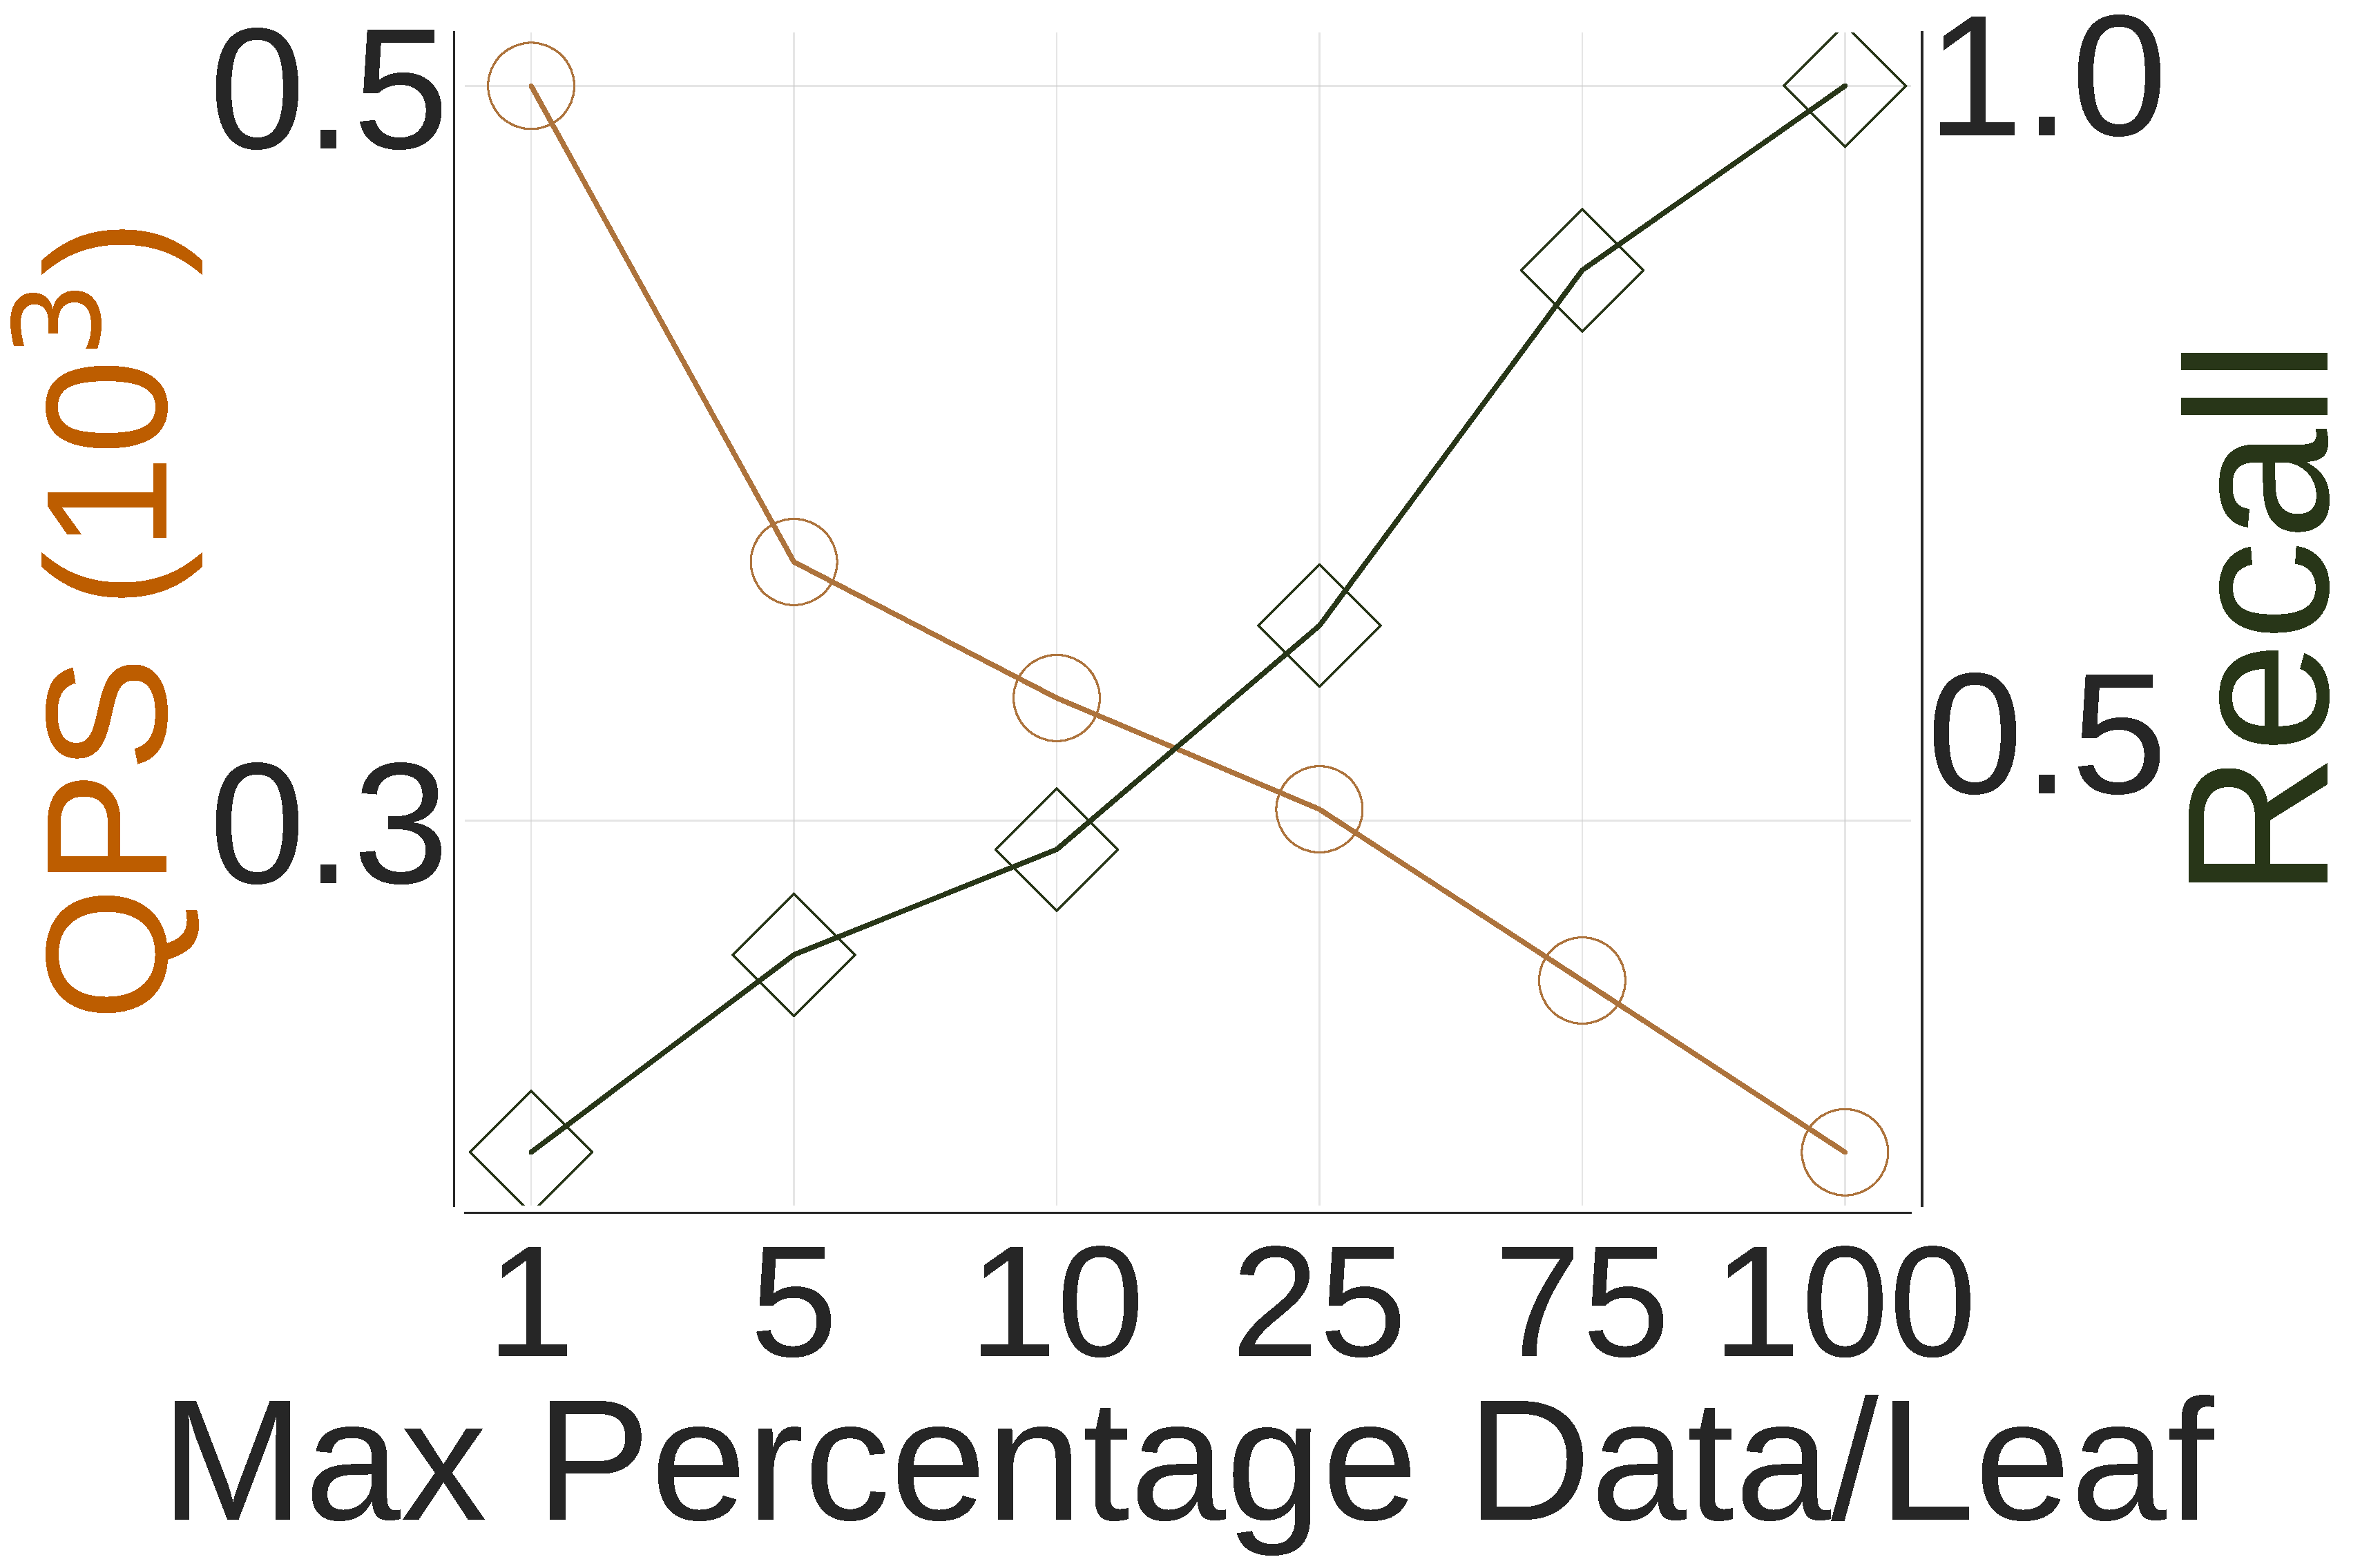
\includegraphics[width=\columnwidth]{../img/elpis/Idx/25_dpl_qps.pdf} 
		\end{subfigure}	
		\caption{{Querying one variable-size cluster (Deep25GB)}}
		\label{fig:elpis:design:cluster-size:errorestqps}
	\end{minipage}
\end{figure}


\subsubsection{Choosing the Number of Clusters}
In this experiment, we show that it is not sufficient to divide the search space to improve the performance of graph-based methods; careful tuning should be applied to find the optimal number of clusters. 
Hercules determines the number of clusters adaptively. It takes as input the maximum amount of data that can fit in one leaf ({\it max\_leaf\_size}), then creates enough leaves to fit similar vectors together in the same leaf. 
Figure~\ref{fig:elpis:design:cluster-size} reports on the x-axis the value of {\it max\_leaf\_size} as a percentage of the size of the dataset, and at the top of each bar, the corresponding number of clusters. 
When the percentage of data is 100, this corresponds to the original HNSW built on the full dataset (i.e., one cluster). 
We observe that splitting the dataset into many small clusters leads to better indexing performance but slower query answering, whereas using a small number of large clusters leads to slower indexing and querying, where the clustering cost becomes marginal compared to the cost of building a graph within each cluster. 
For our experiments, we choose {\it max\_leaf\_size} to be between 5\% and 10\% of the dataset size since it leads to the best trade-off. 
Additionally, we ran an experiment where we vary the size of the clusters and perform the ELPIS search algorithm only on one cluster, keeping all other parameters fixed. 
Figure~\ref{fig:elpis:design:cluster-size:errorestqps} indicates that as the size of a cluster increases, the accuracy improves, but throughput (expressed in Queries Per Second (QPS)) decreases.


\subsection{Index Construction Performance}
We now evaluate the indexing performance of the ten state-of-the-art vector search methods.
We vary the dataset size and report both the indexing total time and footprint. We conduct the experiment using different datasets but, for the sake of space, only report the results for the Deep dataset. The trends are the same across different datasets. The full results can be found in~\cite{url/GASS}.
We use different subsets of the Deep dataset, ranging in size from 1 million to 1 billion vectors, the latter is equivalent to ~350GB. We build the indexes such that each algorithm can achieve a search accuracy of 0.99. 
We first experiment on 1 million vector datasets, reporting results for all methods. However, some methods do not scale to larger sizes and are omitted from the plots. Specifically, on the 25GB datasets, HCNNG, SPTAG-BKT, and SPTAG-KDT exceed 24 hours during index building. Additionally, KGraph and EFANNA require over 300GB and 1.4TB of RAM for 25GB and 100GB datasets, respectively. Consequently, DPG, NSG, and SSG (as they use KGraph and EFANNA) are also omitted from 100GB and larger datasets.



\noindent{\bf Indexing Time.} Figure~\ref{fig:elpis:idx:time} demonstrates that II-based approaches boast the lowest overall indexing time across various dataset sizes. Specifically, the II and DC-based approach, ELPIS, shows significant advantages, being 2.7x faster than HNSW and 4x faster than NSG for both 1M and 25GB dataset sizes. Note that NSG's indexing time includes both the construction of its base graph, EFANNA, which is time-intensive, and the refinement with NSG. SPTAG-BKT and SPTAG-KDT exhibit high indexing times, requiring over 25 hours to index Deep25GB dataset—24 times more than ELPIS, the fastest method. This inefficiency in SPTAG arises from its design, which involves constructing multiple TP Trees and graphs, becoming increasingly costly with larger datasets. On larger datasets 100GB and 1B vectors ($\approx$350GB), only HNSW, ELPIS, and Vamana scale with acceptable indexing time, with ELPIS being 2 and 2.7 times faster than HNSW and Vamana, respectively.


\noindent\textbf{Indexing Footprint.}
Figure~\ref{fig:elpis:idx:footprint:memory} reports the memory footprint for each indexing structure, including the raw data storage. To perform the evaluation, we record the peak virtual memory usage during the index-building phase\footnote{Readings are taken from the proc pseudo filesystem’s Virtual Memory Peak.}. SPTAG-BKT and SPTAG-KDT demonstrate substantial efficiency in memory utilization despite having the highest indexing time. 

They exhibit the lowest indexing memory footprint for 1M and 25GB datasets. For larger datasets, ELPIS has the lowest indexing memory footprint, occupying up to 40\% less memory than HNSW and 30\% less than Vamana during indexing. This is because ELPIS needs a smaller maximum outdegree and beam width compared to its competitors to efficiently build the index. HNSW has a higher indexing memory footprint due to its use of a graph layout optimized for direct access to node edges through a large contiguous block allocation~\cite{url/hnsw}. This layout offers a time advantage over adjacency lists by reducing memory indirections and cache misses. However, it can result in quadratic memory growth when using a large maximum outdegree on large-scale datasets. 
In Figure \ref{fig:elpis:idx:footprint:disk}, we compare the size of method indices, including the raw data. The figure shows that certain methods, such as EFANNA, HCNNG, KGraph, and consequently NSG, SSG, and DPG (which use one of these base graphs), exhibit a significantly larger memory footprint relative to their final index size. For instance, HCNNG consumes substantial memory during indexing, requiring over 200GB for Deep25GB (Fig. \ref{fig:elpis:idx:footprint:memory}) due to merging multiple MST from numerous samples generated during hierarchical clusterings. In contrast, its final index size is less than 50GB (Fig. \ref{fig:elpis:idx:footprint:disk}).

\begin{figure}[!htb]
	\captionsetup{justification=centering}
	\centering	
	\begin{minipage}{\textwidth}
		\begin{subfigure}{\textwidth}
			\centering
			\captionsetup{justification=centering}				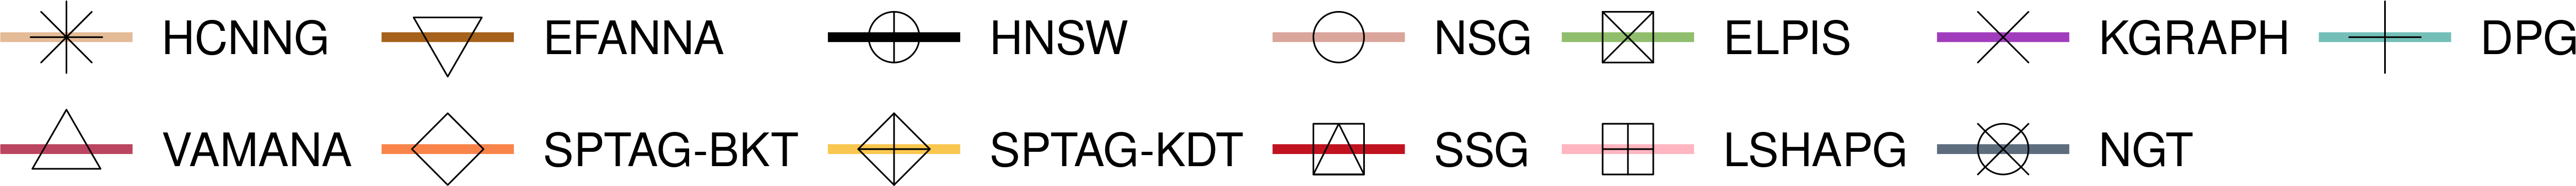
\includegraphics[width=\textwidth]{../img/Experiments/legendall.png}
		\end{subfigure}\\
		\vspace{-0.3cm}
	\end{minipage}
	\begin{minipage}{0.28\textwidth}				
	%	\captionsetup{justification=centering}
			\centering
		\begin{subfigure}{\textwidth}
			\captionsetup{justification=centering}	
			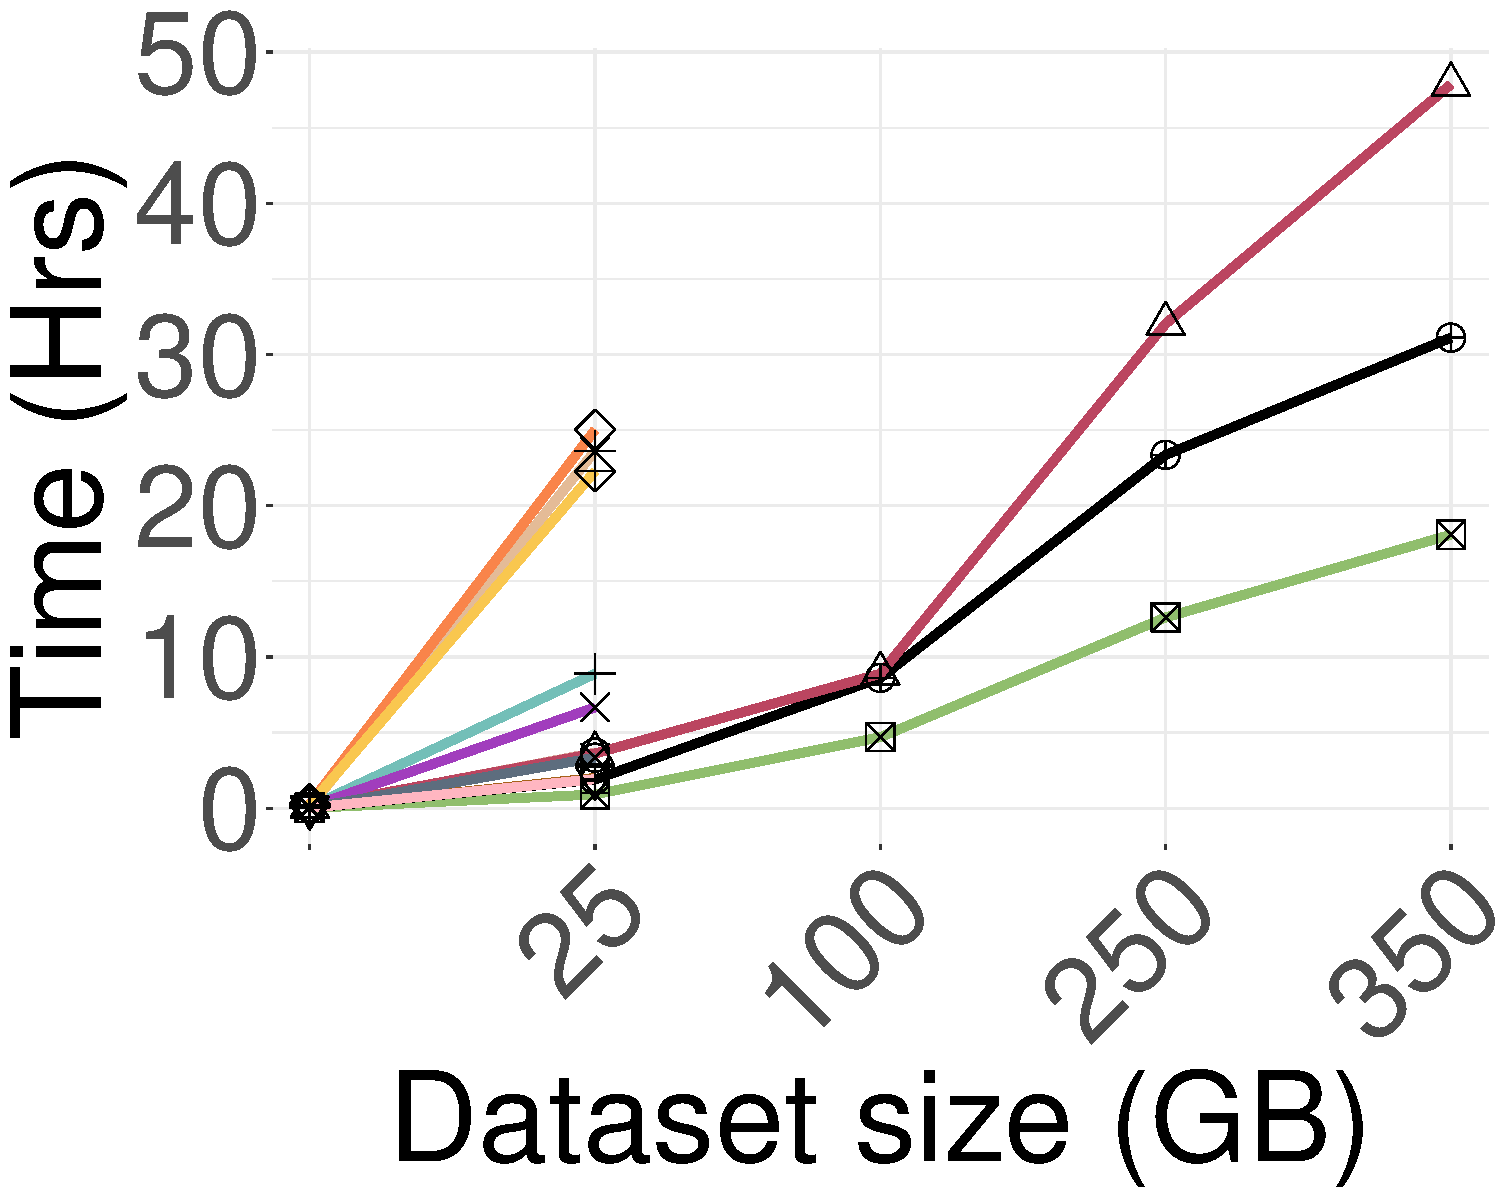
\includegraphics[width=\textwidth]{../img/Experiments/Idx_footprint_datasets/idx_time_deep_n.pdf}
		\end{subfigure}	
		\caption{{Indexing Time}}
		\label{fig:elpis:idx:time}
	\end{minipage}	
 \hspace{0.15in}
	\begin{minipage}{0.28\textwidth}				
	%	\captionsetup{justification=centering}
		\begin{subfigure}{\textwidth}
			\centering
			\captionsetup{justification=centering}	
			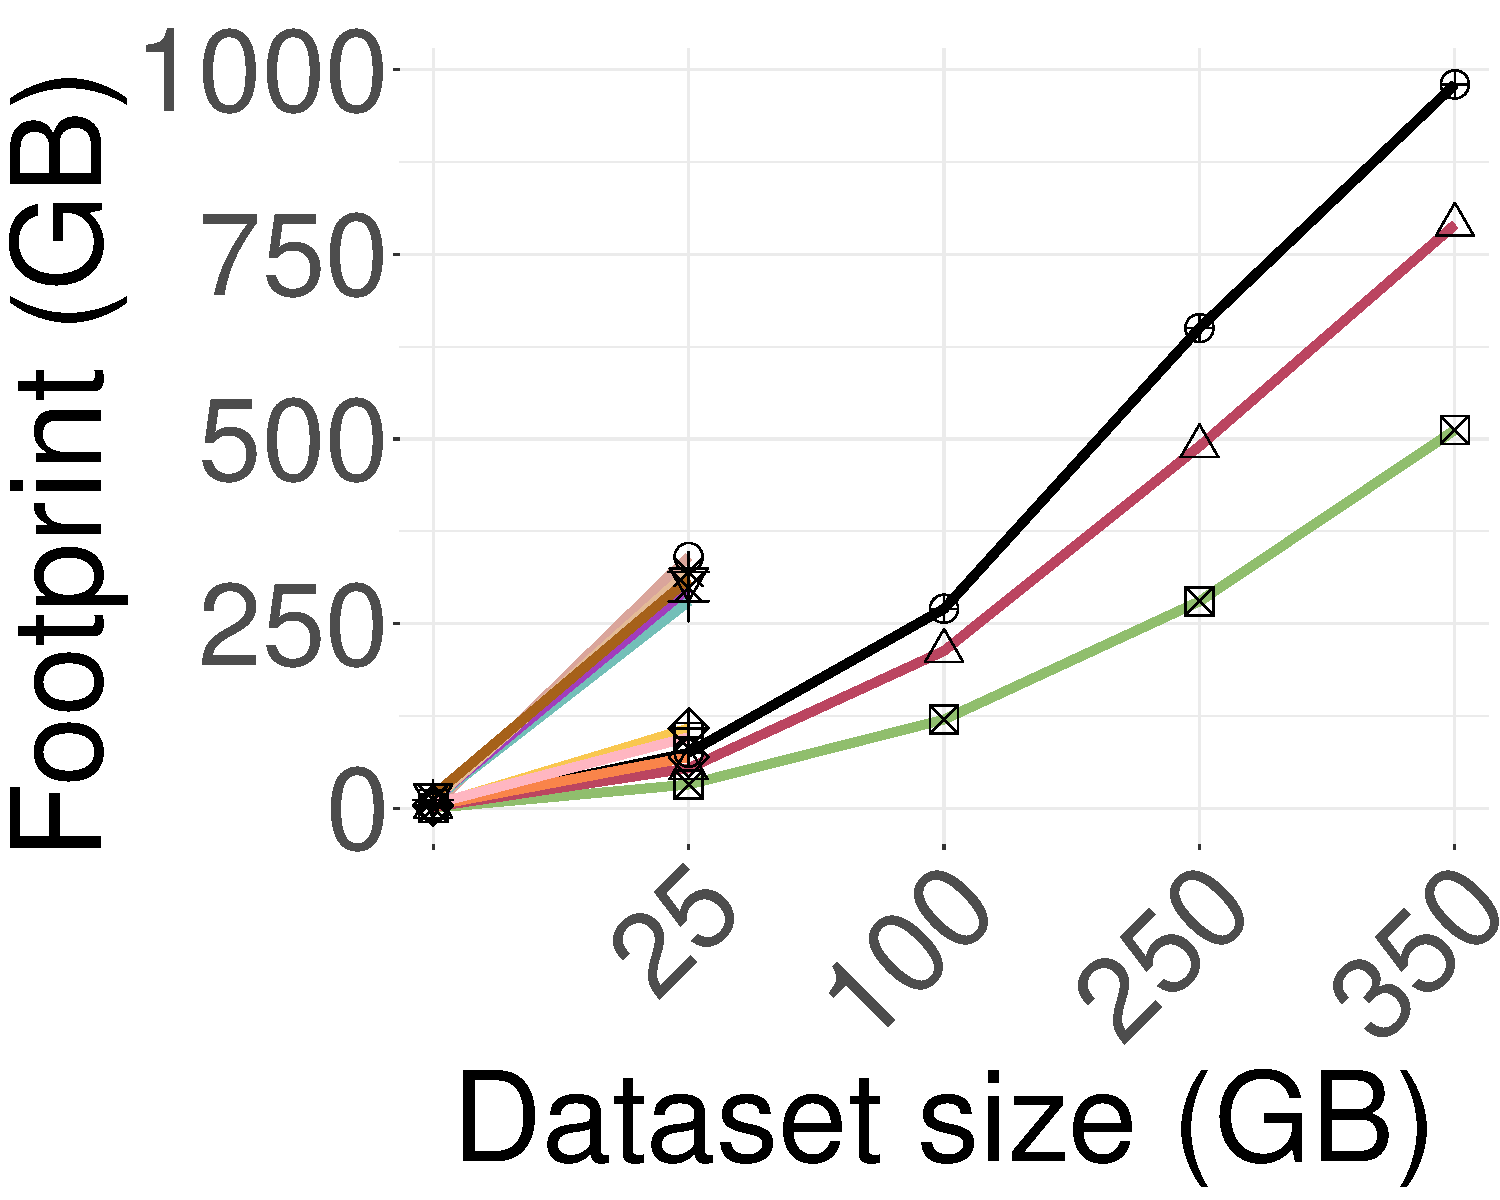
\includegraphics[width=\textwidth]{../img/Experiments/Idx_footprint_datasets/idx_footprint_deep_n.pdf}
		\end{subfigure}	
		\caption{{Indexing Memory Footprint}}
		\label{fig:elpis:idx:footprint:memory}
	\end{minipage}	
 \hspace{0.15in}
	\begin{minipage}{0.29\textwidth}				
	%	\captionsetup{justification=centering}
		\begin{subfigure}{\textwidth}
			\centering
			\captionsetup{justification=centering}	
			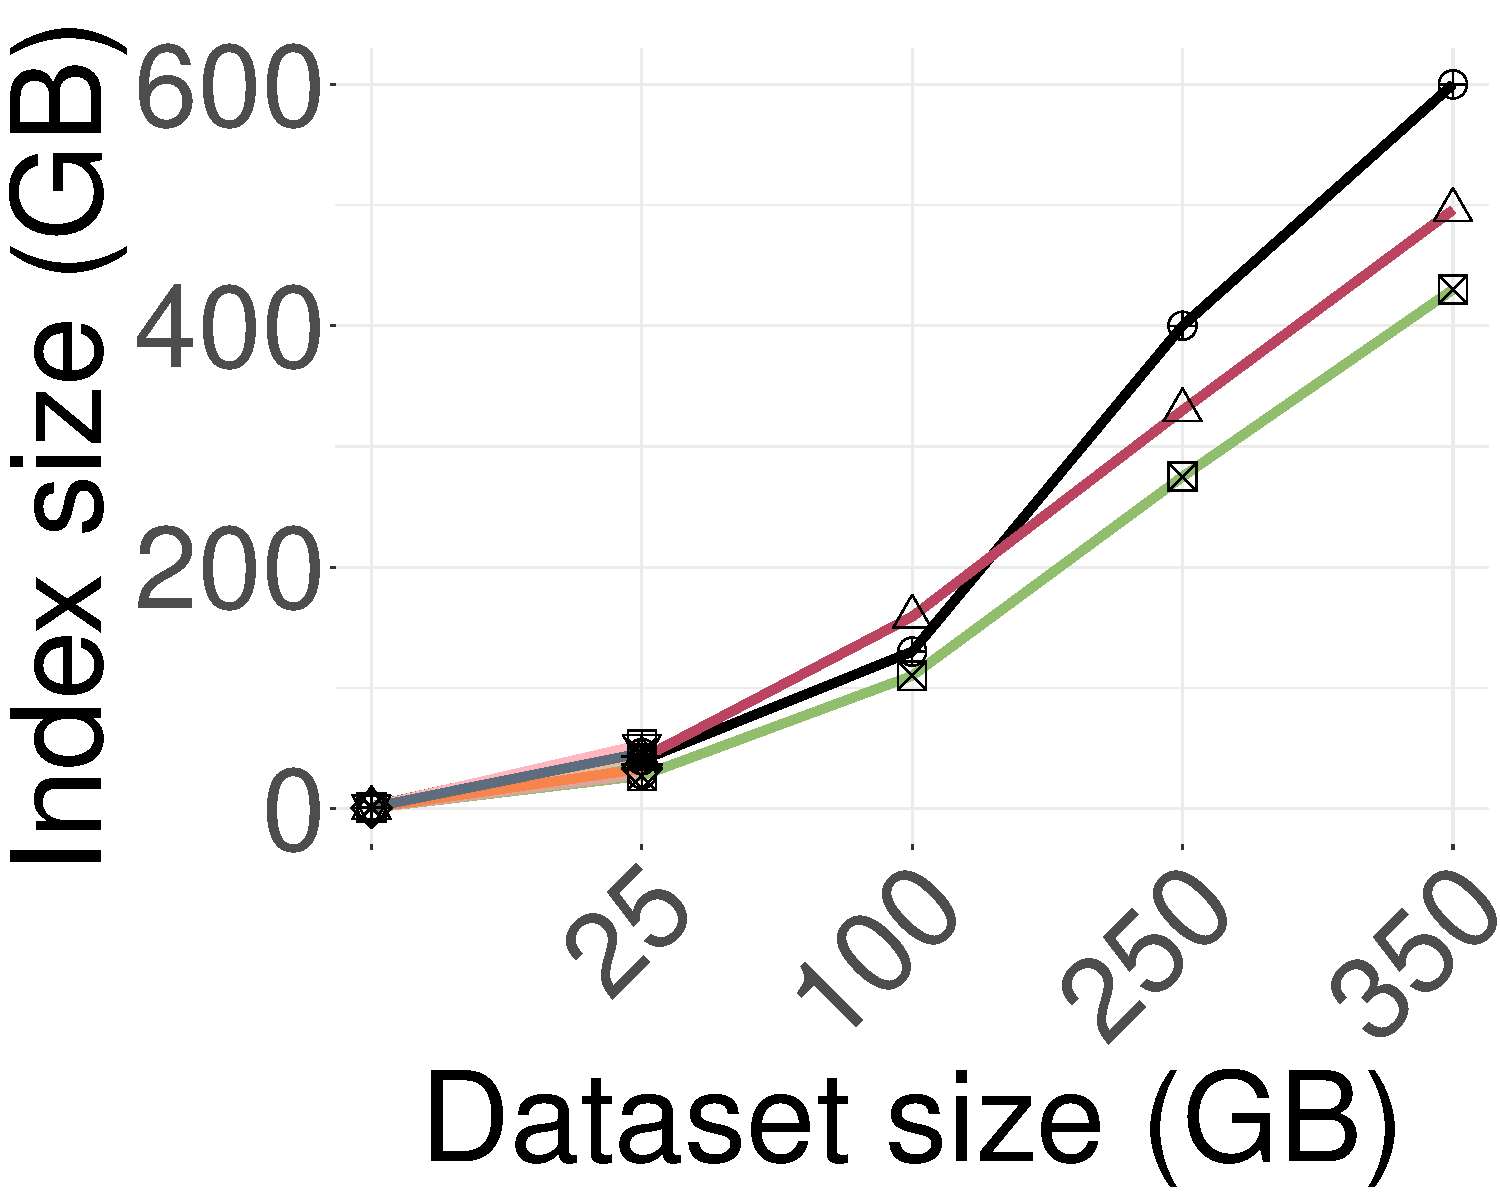
\includegraphics[width=\textwidth]{../img/Experiments/Idx_footprint_datasets/idx_indexsize_deep_n.pdf}
		\end{subfigure}	
		\caption{{Indexing Disk Footprint}}
		\label{fig:elpis:idx:footprint:disk}
	\end{minipage}		
	\begin{minipage}{0.28\textwidth}				
		%	\captionsetup{justification=centering}
		\begin{subfigure}{\textwidth}
			\centering
			\captionsetup{justification=centering}	
			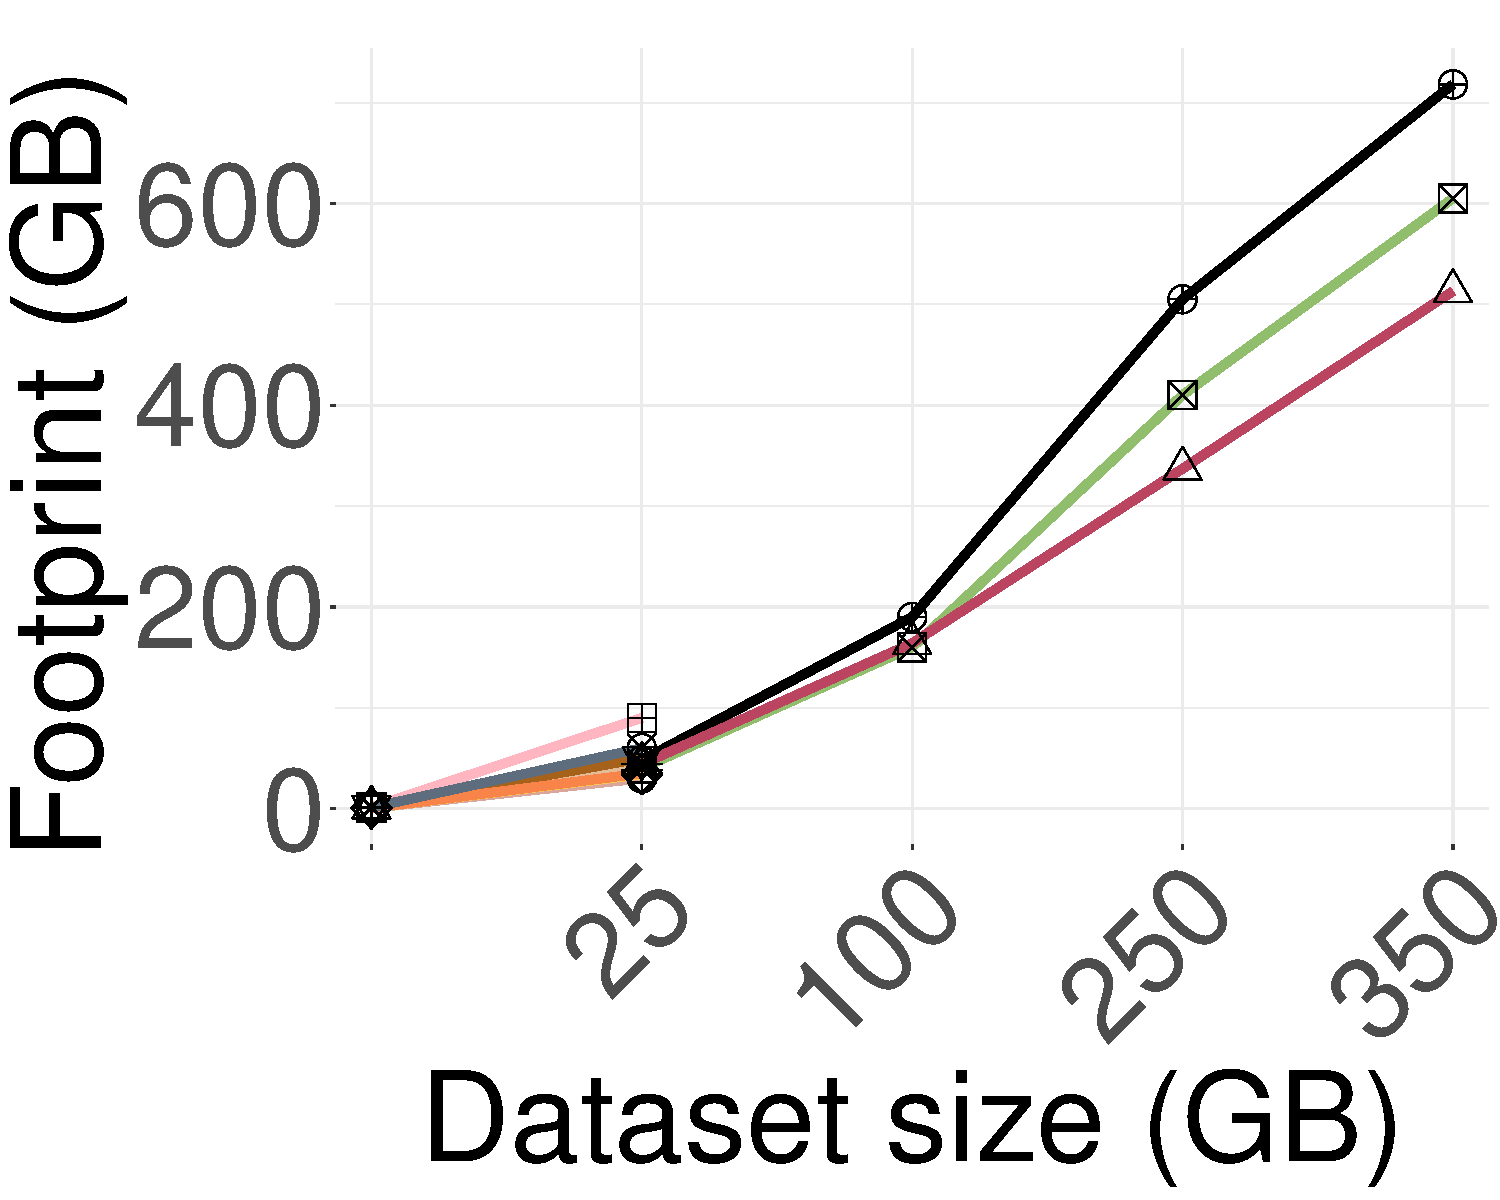
\includegraphics[width=\textwidth]{../img/Experiments/Idx_footprint_datasets/search_footprint_deep_n.pdf}
		\end{subfigure}	
		\caption{{Query Memory Footprint}}
		\label{fig:elpis:query:footprint:memory}
	\end{minipage}	
 \hspace{0.15in}
	\begin{minipage}{0.28\textwidth}
		\centering
		\begin{subfigure}{\textwidth}
			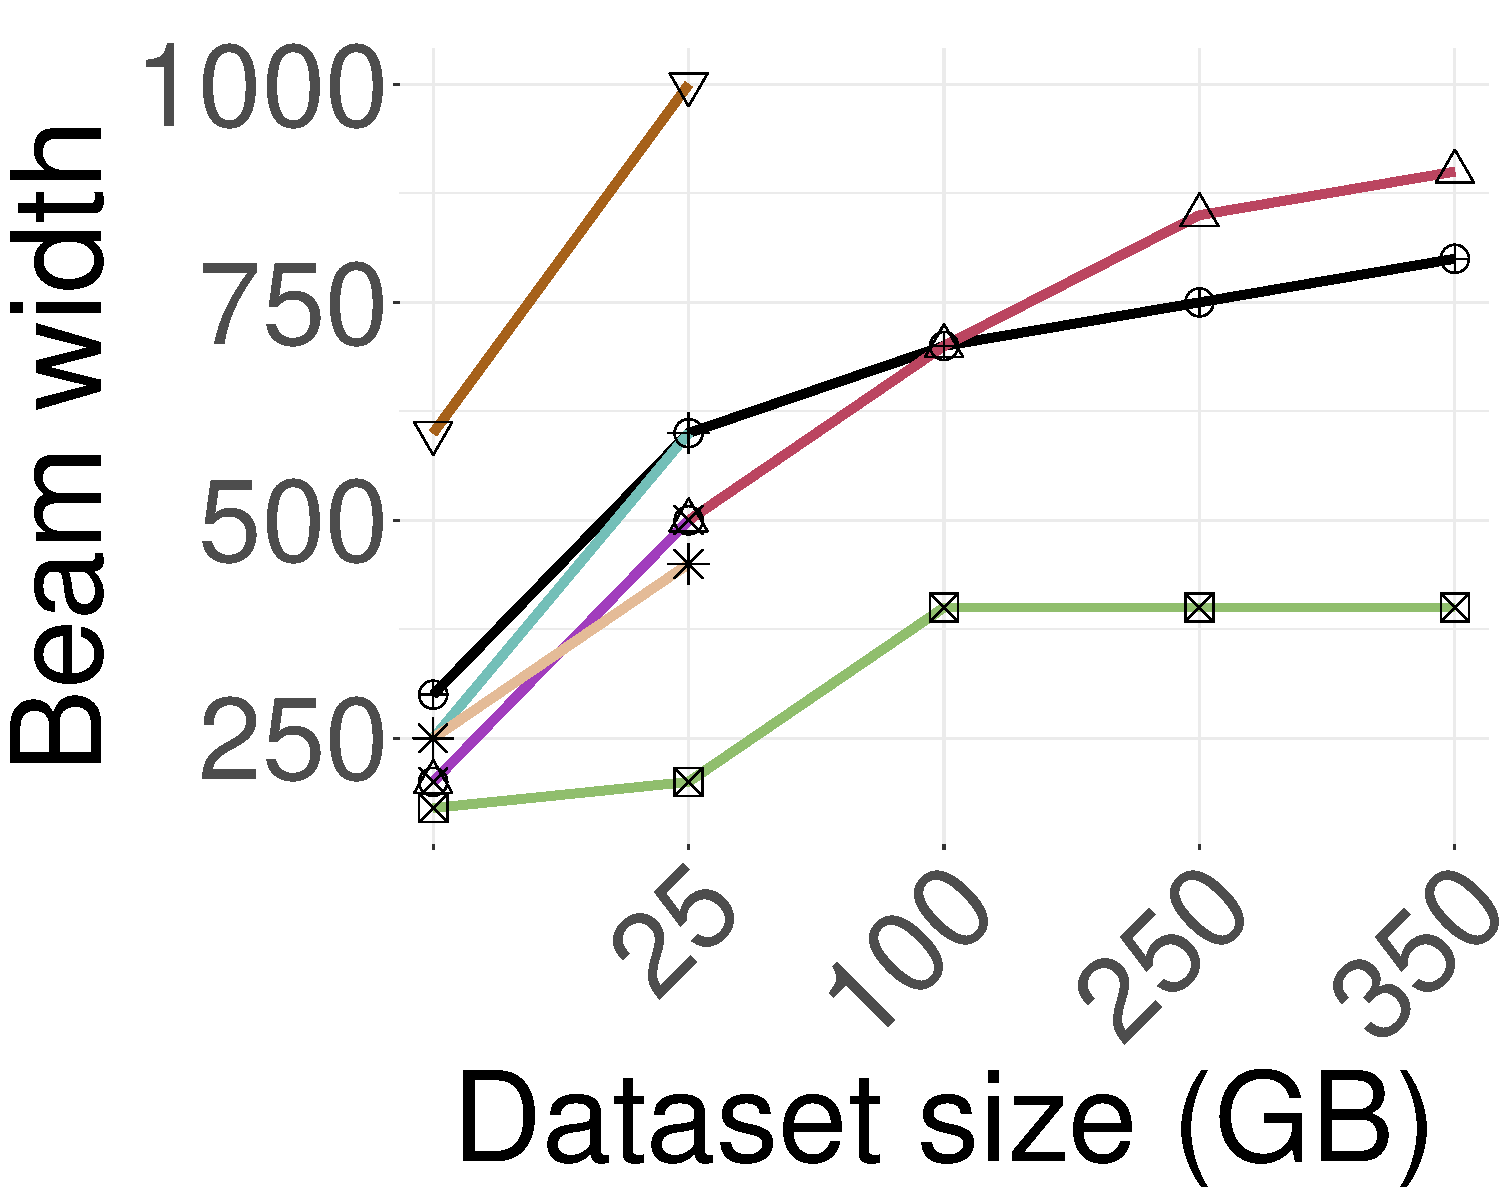
\includegraphics[width=\textwidth]{../img/Experiments/Idx_footprint_datasets/qrs_beamwidth_n.pdf}
		\end{subfigure} 
		\caption{{Query Beam Width}}
		\label{fig:elpis:query:beam-width}
	\end{minipage}
\end{figure}

\subsection{Search Performance}
We now evaluate the query-answering performance of the different methods. Some methods are omitted because the indexes could not be built on large datasets (NSG, SSG, SPTAG-BKT, DPG, EFANNA, SPTAG-KDT, HCNNG, KGraph). Other methods were not included in some 25GB plots (KGraph, DPG, SPTAG-KDT, HCNNG, and EFANNA) for the sake of clarity since their query-answering times were significantly higher than the best baselines. The full results can be found in~\cite{url/GASS}.  

\noindent\textbf{Query Memory Footprint and Beam Width.} 
Figure~\ref{fig:elpis:query:footprint:memory} for the Deep dataset indicates that Vamana, followed by ELPIS, have the lowest memory footprint during search. Even though ELPIS has a smaller index size, it adopts a contiguous memory storing during search, which increases the index footprint when loaded into memory. Besides, Figure~\ref{fig:elpis:query:beam-width} shows that ELPIS requires the smallest beam width to reach similar query accuracy. A very high beam width indicates that the beam search needs to visit a wider area and make more distance calculations to retrieve the nearest neighbor (NN) answers.

\noindent\textbf{Real Datasets.}  On the datasets with 1M vectors (Figure~\ref{fig:elpis:query:performance:1M}), ELPIS and NSG are the best performers on Sift1M and Seismic1M. NSG maintains its leading position in Deep1M, while HCNNG shows the best performance for SALD1M. 

When moving to 25GB datasets (Figure~\ref{fig:elpis:query:performance:25GB}), SSG and HCNNG experience a drop in performance, and ELPIS takes the lead with the best overall performance, except for SALD25GB, where SPTAG-BKT wins on high accuracy. It is worth noting that none of the methods achieved an accuracy over 0.8 on the Seismic dataset, leading us to report results for these lower recall values. The significant indexing footprint of NSG prevented us from extending its evaluation to larger datasets, as constructing the EFANNA graph (which NSG depends on) requires more memory than the available 1.4TB. 

For hard query workloads in Figure~\ref{fig:search:query:performance:25GB:hard}, we compare the best-performing methods from the two most performing graph paradigms, ND-based and DC-based methods, including HNSW, NSG, ELPIS, and SPTAG-BKT. SPTAG-BKT achieves the overall best performance for the 1\% noise query set. As we increase the noise up to 10\%, SPTAG-BKT's performance deteriorates, which we can attribute to the SPTAG-BKT structure failing to identify good seed points. At the same time, the other competitors gain an advantage, with ELPIS taking the lead. 

When analyzing very large datasets of 1 billion vectors, Figure~\ref{fig:elpis:query:performance:1B} shows the superiority of ELPIS, which is up to an order of magnitude faster at achieving 0.95 accuracy, thanks to its design that supports multi-threading for query answering. This trend is consistent across subsets ranging from 100GB (Figure~\ref{fig:elpis:query:performance:100GB}) to 250GB (detailed results are reported in~\cite{url/GASS}).

\noindent{\bf Data Distributions.} We assess top performers from different classes of paradigms (EFANNA, Vamana, SSG, HNSW, ELPIS, and SPTAG-BKT) on challenging datasets (Fig.~\ref{fig:datacomp}) and report the results in Figures~\ref{fig:query:performance:25GB:rand:pow1:10NN} and~\ref{fig:query:performance:25GB:rand:pow50:10NN}. We observe that ELPIS consistently achieves high accuracy across skewness levels (0 to 50), outperforming other methods. As dataset skewness increases and search becomes easier, most graph-based approaches improve, but ELPIS still maintains its superiority.


\newcommand{\soneM}{0.28}
\newcommand{\spbf}{0.13in}
\begin{figure}[!htb]
	\captionsetup{justification=centering}
	\centering
		\begin{subfigure}{\textwidth}
			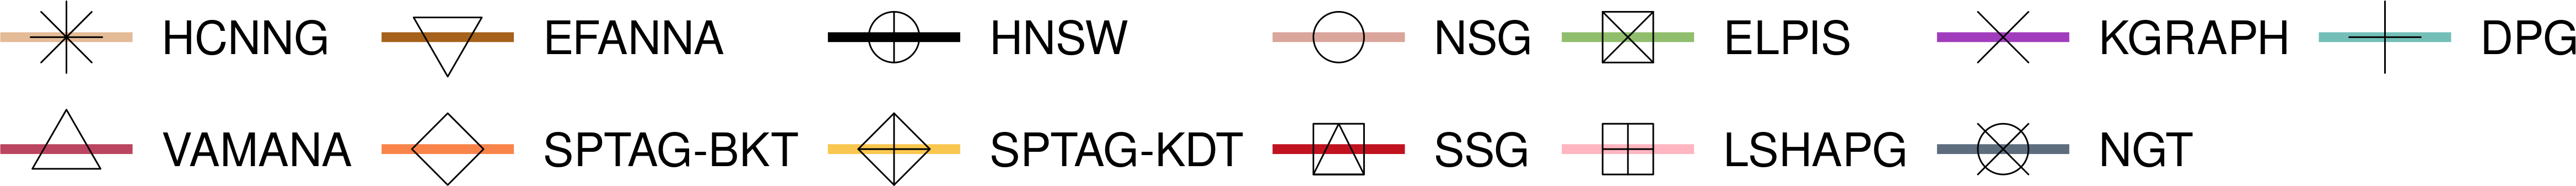
\includegraphics[width=\textwidth]{../img/Experiments/legendall.png}
		\end{subfigure}	
  
	\captionsetup[subfigure]{justification=centering}
	\begin{subfigure}{\soneM\textwidth}
		\centering
		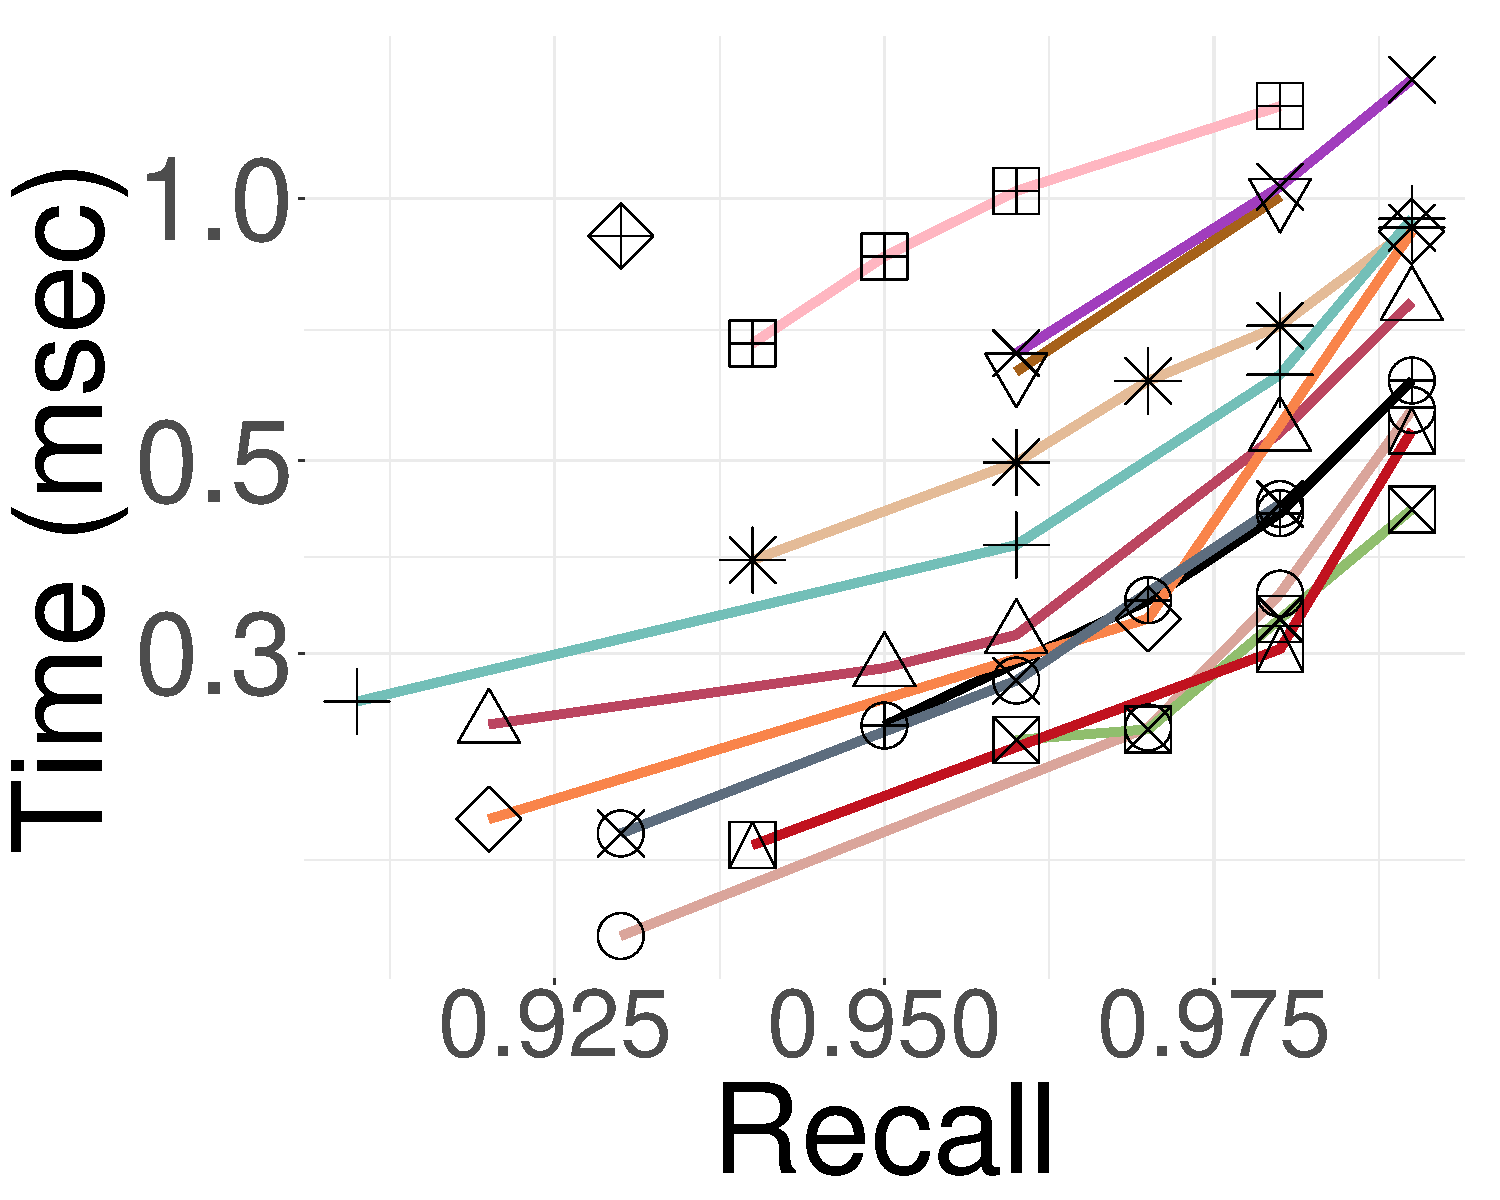
\includegraphics[width=\textwidth]{../img/Experiments/search/1M/sift_10nn.pdf}
		\caption{\textbf{Sift1M}} 
	
 \label{fig:elpis:query:performance:1M:sift:10NN}
	\end{subfigure}
   \hspace{0.4cm}
	\begin{subfigure}{\soneM\textwidth}
		\centering
		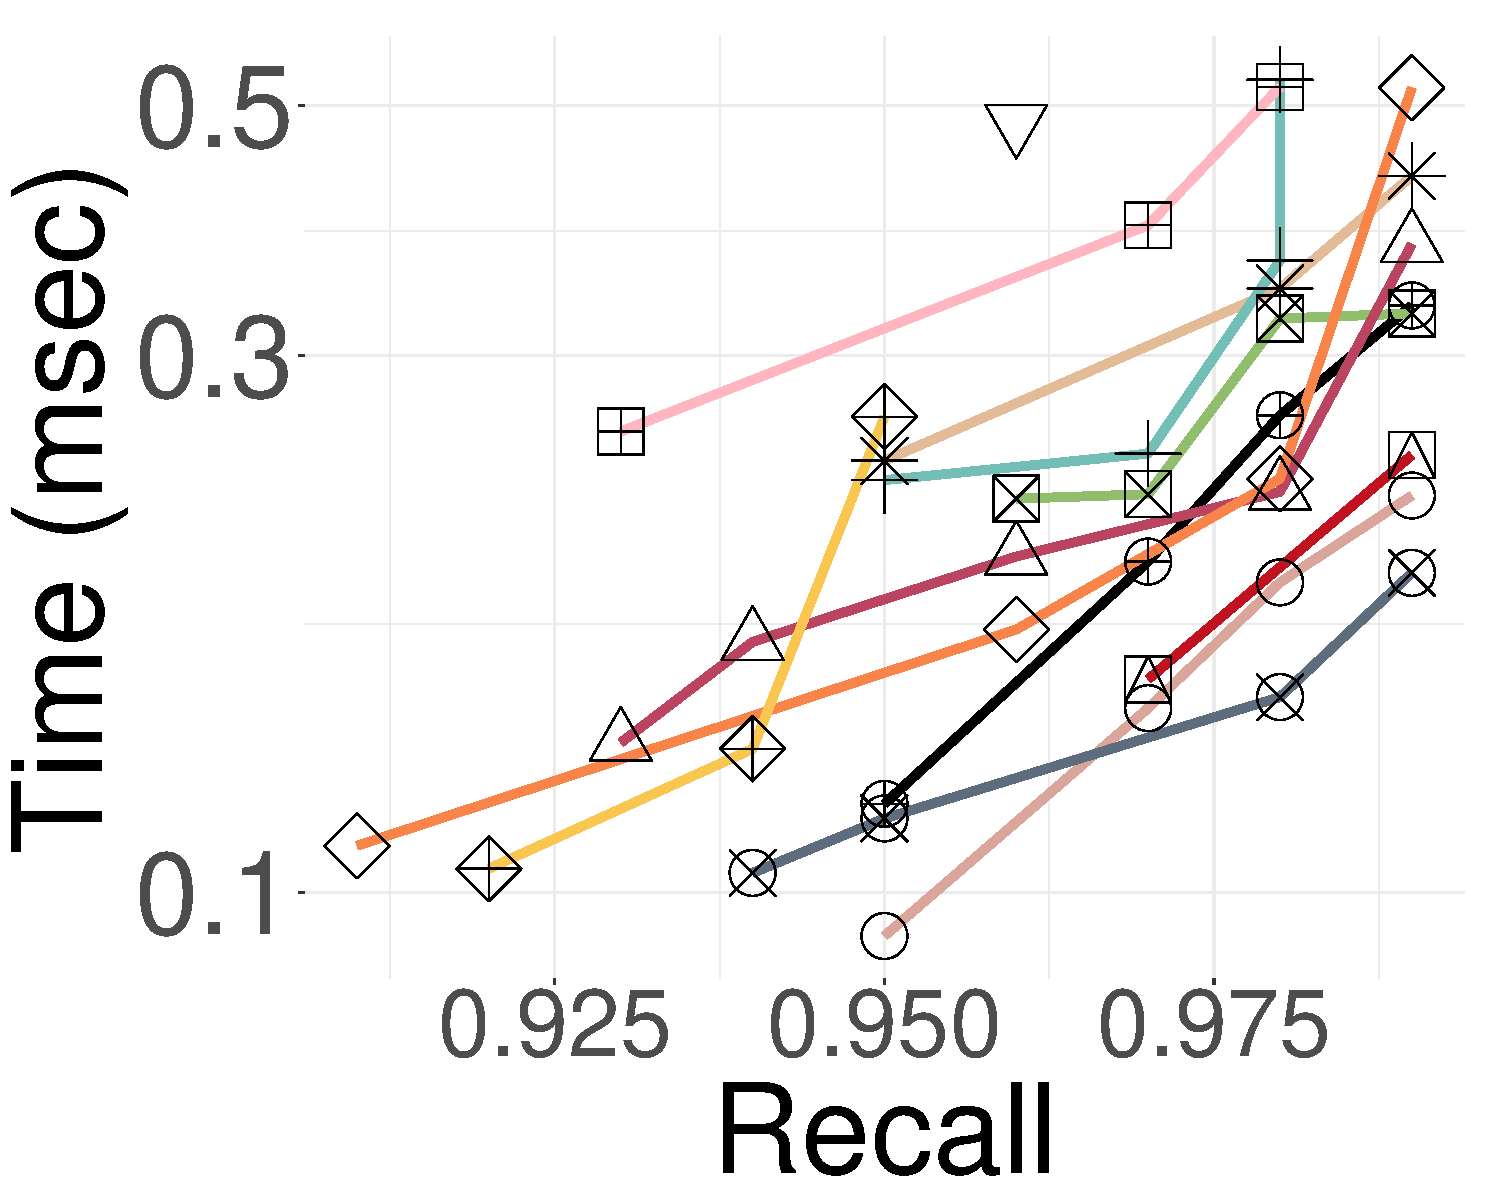
\includegraphics[width=\textwidth]{../img/Experiments/search/1M/deep_10nn.pdf}
		\caption{\textbf{Deep1M}} 
		\label{fig:elpis:query:performance:1M:deep:10NN}
	\end{subfigure}
   \hspace{0.4cm}
	\begin{subfigure}{\soneM\textwidth}
		\centering
		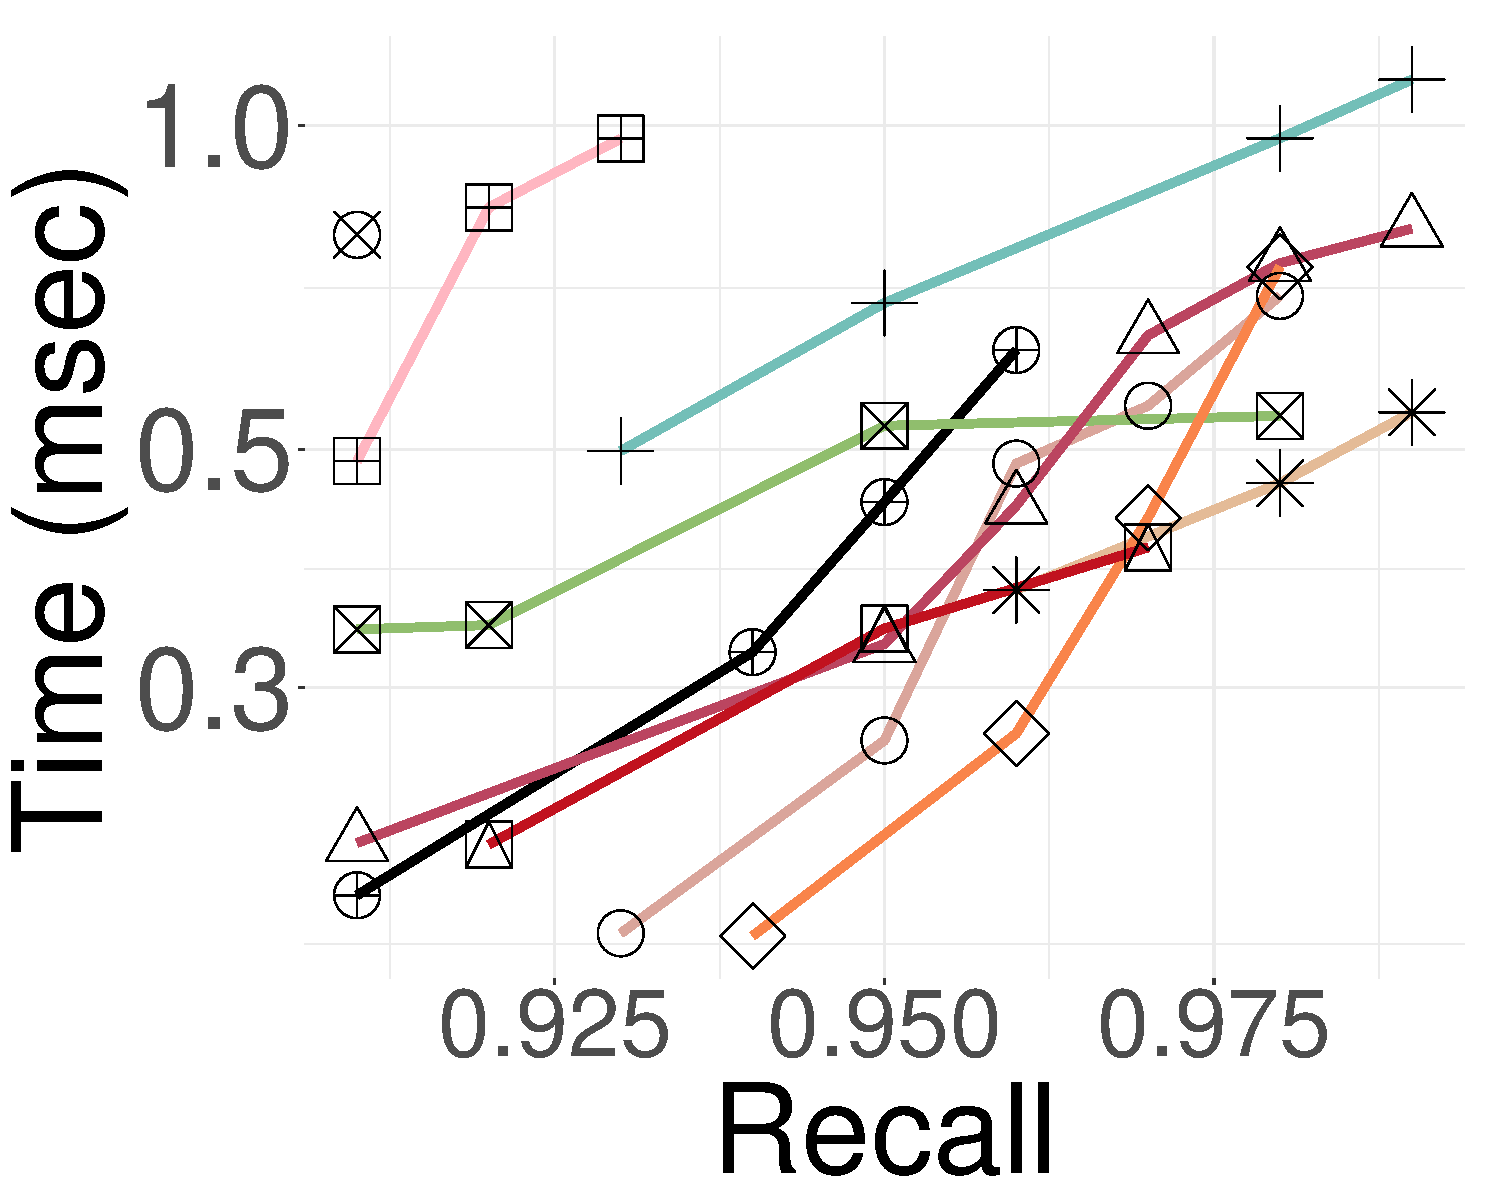
\includegraphics[width=\textwidth]{../img/Experiments/search/1M/sald_10nn.pdf}
		\caption{\textbf{SALD1M}} 
		\label{fig:elpis:query:performance:1M:sald:10NN}
	\end{subfigure}
 
	\begin{subfigure}{\soneM\textwidth}
		\centering
		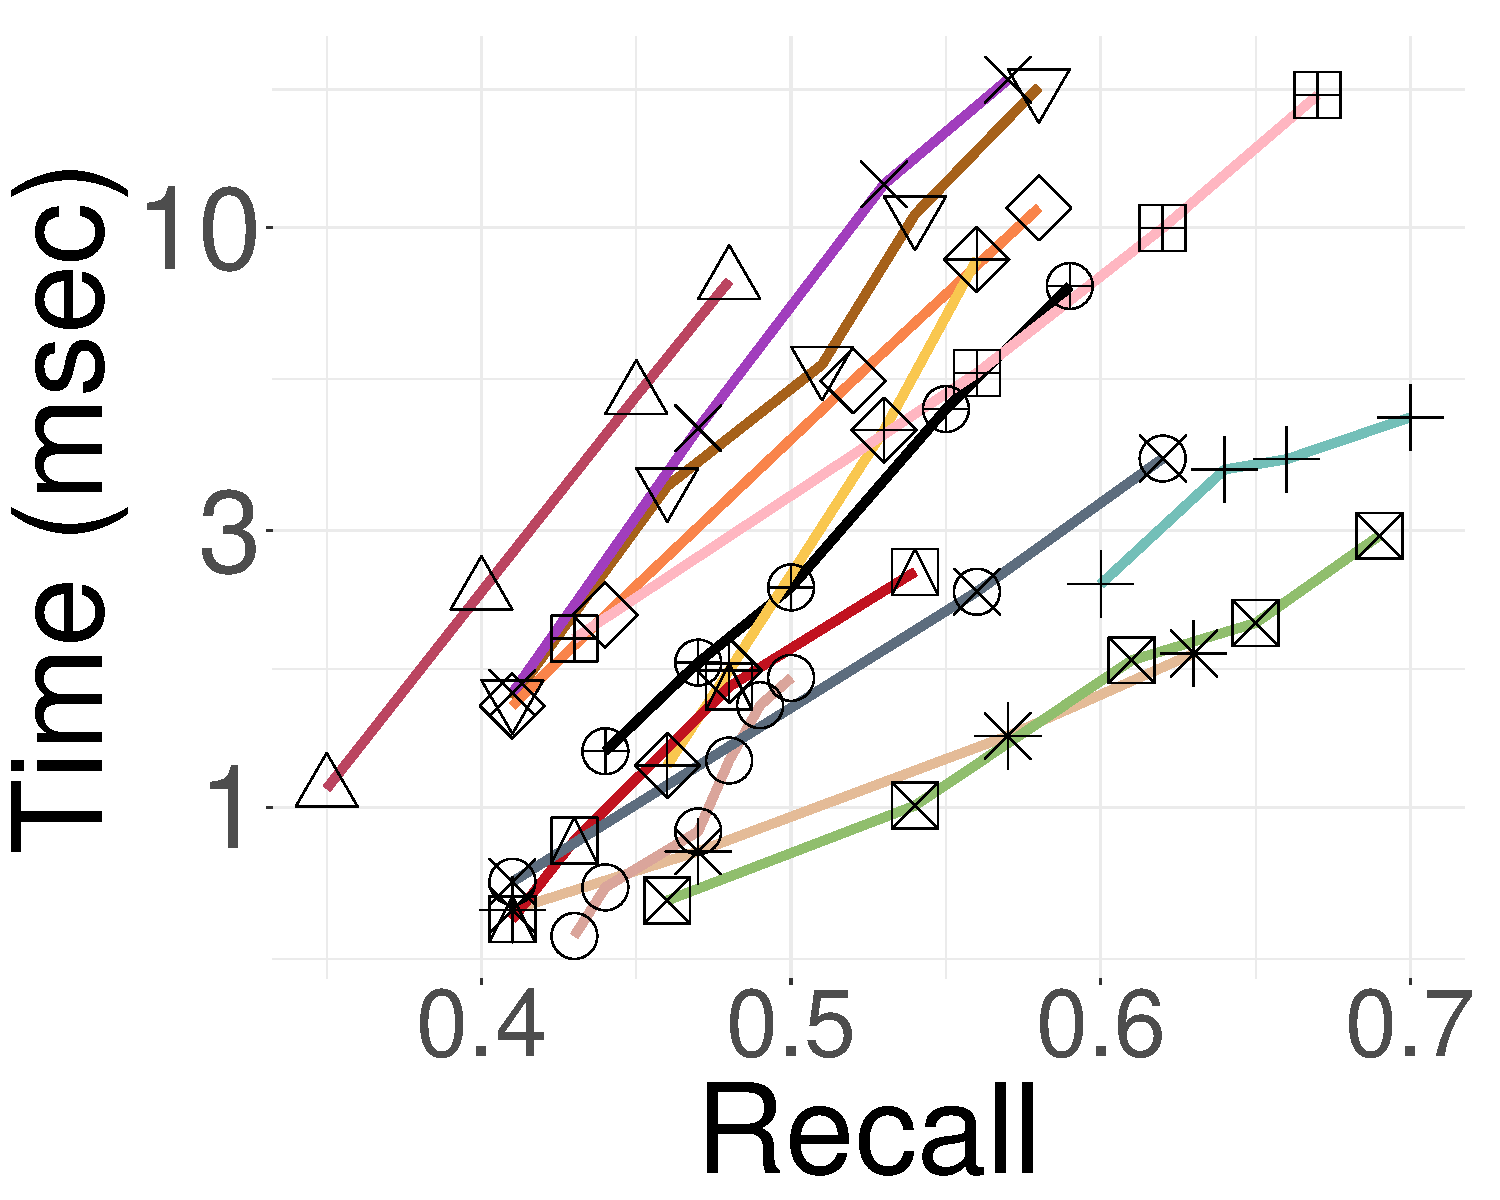
\includegraphics[width=\textwidth]{../img/Experiments/search/1M/seismic_10nn.pdf}
		\caption{\textbf{Seismic1M}} 
		\label{fig:elpis:query:performance:1M:seismic:10NN}
	\end{subfigure}
   \hspace{0.4cm}
	\begin{subfigure}{\soneM\textwidth}
		\centering
		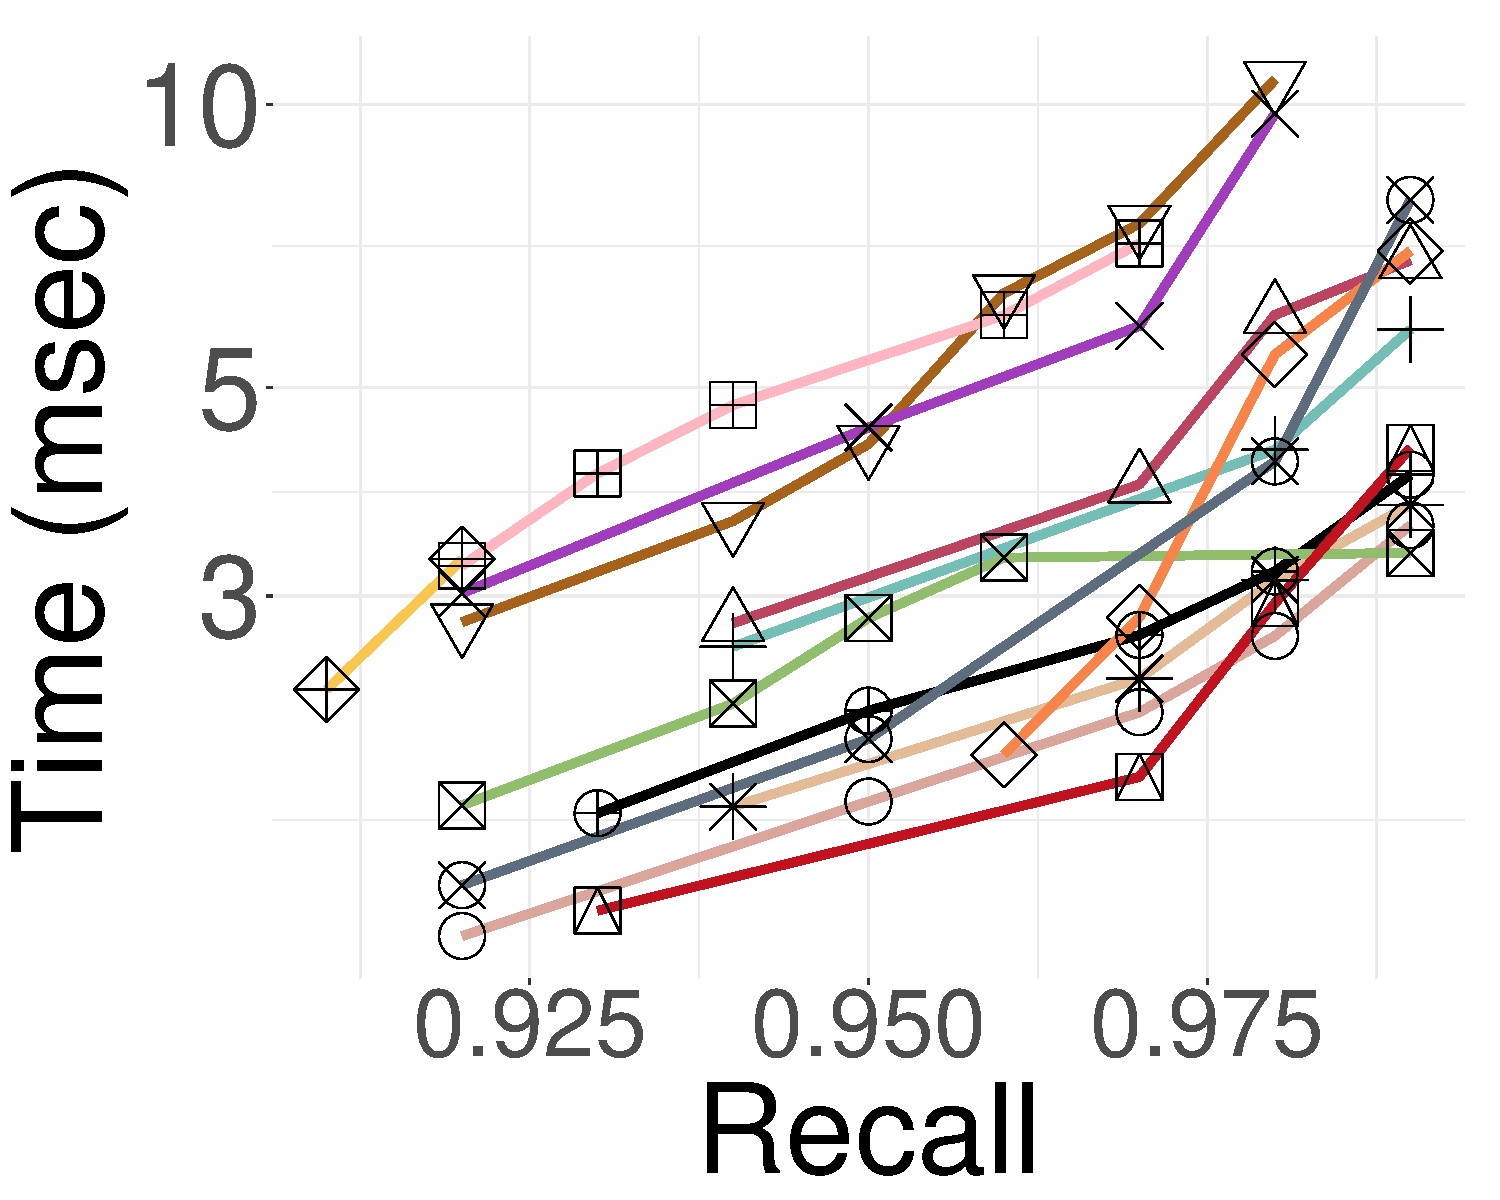
\includegraphics[width=\textwidth]{../img/Experiments/search/1M/gist_10nn.pdf}
		\caption{\textbf{Gist1M}} 
		\label{fig:elpis:query:performance:1M:gist:10NN}
	\end{subfigure}
   \hspace{0.4cm}
 	\begin{subfigure}{\soneM\textwidth}
		\centering
		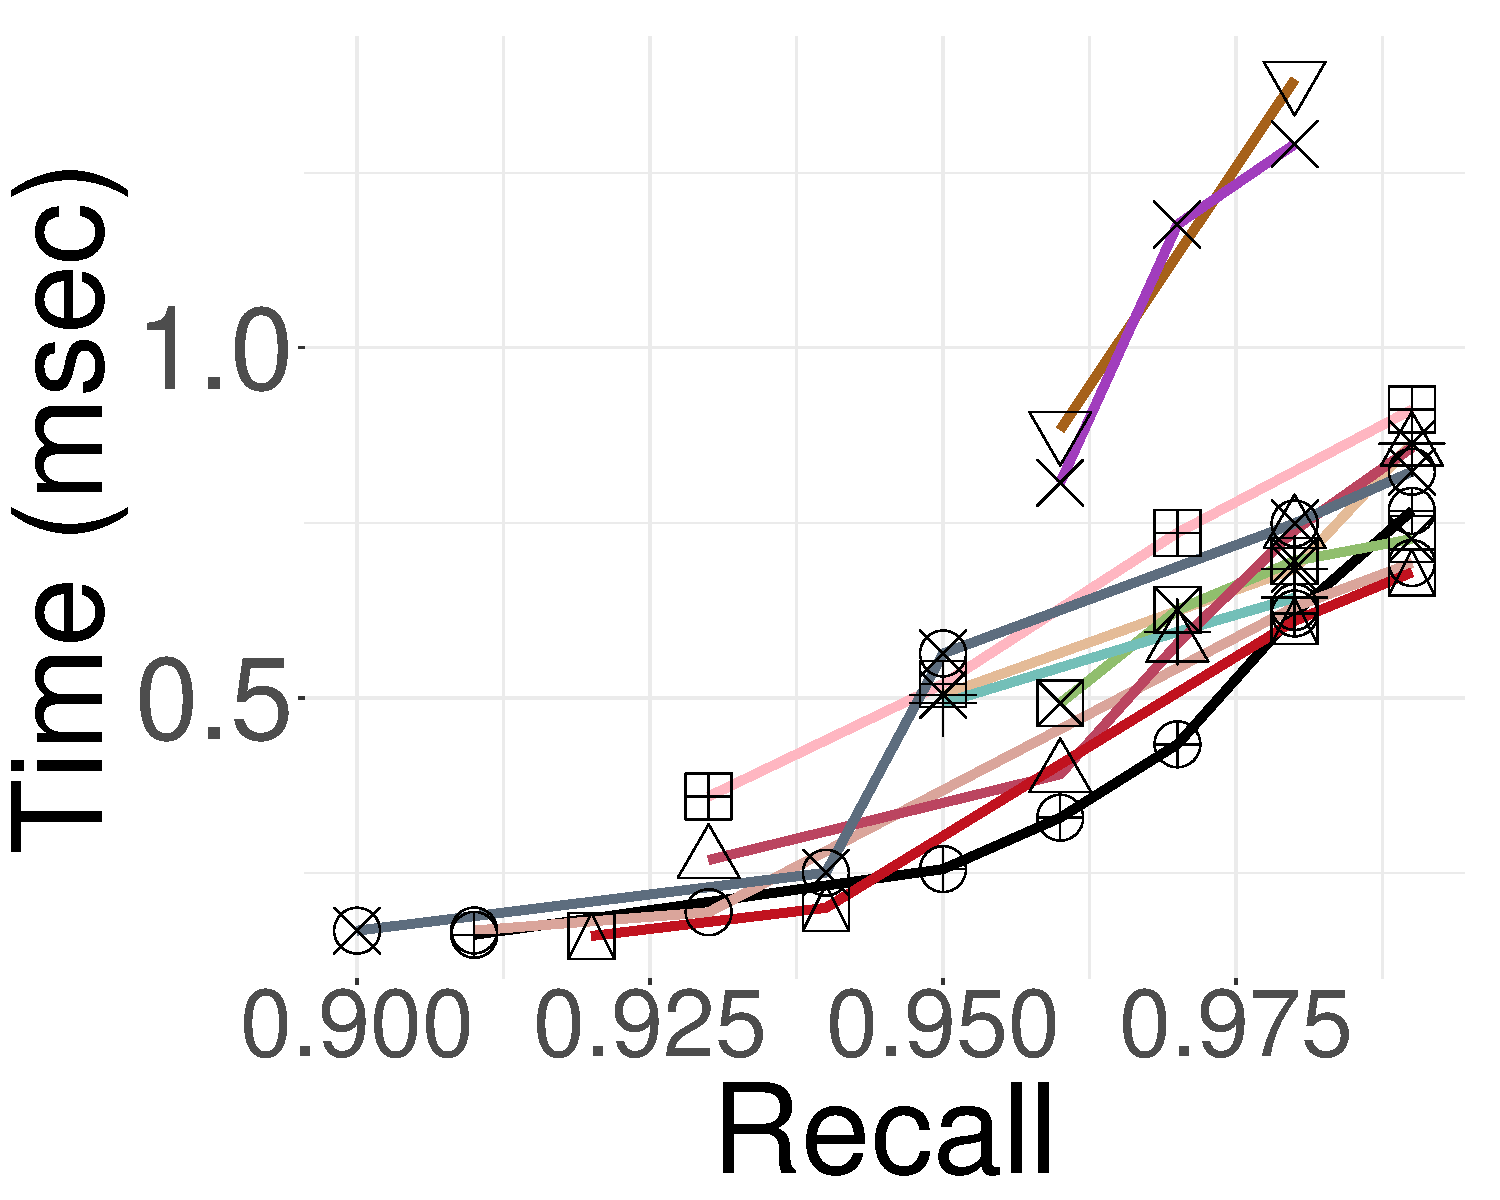
\includegraphics[width=\textwidth]{../img/Experiments/search/1M/imagenet_10nn.pdf}
		\caption{\textbf{ImageNet1M}} 
		\label{fig:elpis:query:performance:1M:imagenet:10NN}
	\end{subfigure}
	\vspace*{-0.2cm}
	%\caption{{\color{black} Efficiency vs. accuracy in memory (100 queries)}}	surat al mulk
	%	\caption{{Efficiency vs. accuracy (Dataset = 1M, Queries = 100, k = 10) }}	
	\caption{Query performance on 1M vectors}	
	\vspace*{-0.2cm}
	\label{fig:elpis:query:performance:1M}
\end{figure}


    \newcommand{\soneMs}{0.155}
\renewcommand{\soneM}{0.25}
\renewcommand{\spbf}{0.0in}
\begin{figure}[!htb]
	\captionsetup{justification=centering}
	\centering
		\begin{subfigure}{\textwidth}
			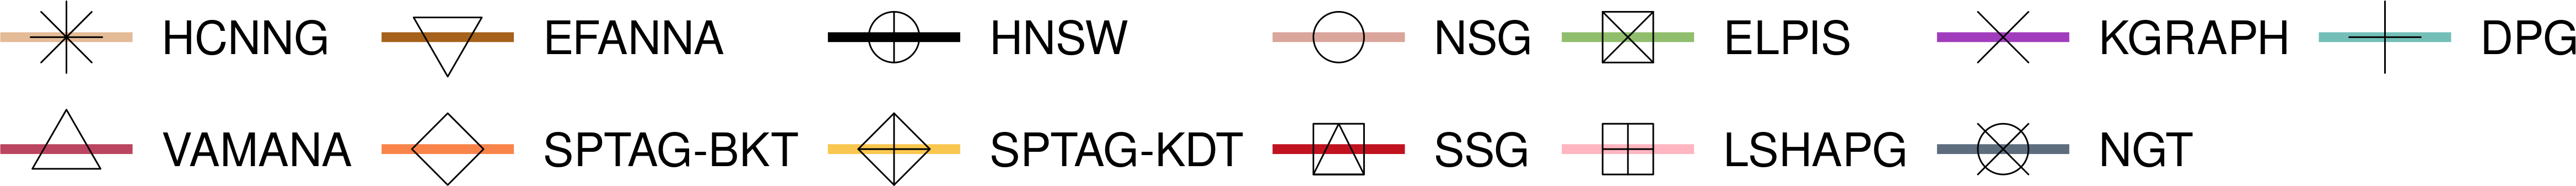
\includegraphics[width=\textwidth]{../img/Experiments/legendall.png}
		\end{subfigure}	
 
	\begin{minipage}{\textwidth}
 \centering
		\captionsetup{justification=centering}
		\captionsetup[subfigure]{justification=centering}
	 \begin{comment}
 \begin{minipage}{0.05\textwidth}
		\captionsetup{justification=centering}
		\captionsetup[subfigure]{justification=centering}
		\begin{subfigure}{\textwidth}
		\vspace*{-.7in}
		
\includegraphics[width=0.6\columnwidth]{../img/Experiments/time.pdf}
		\vspace*{.6in}
		
\includegraphics[width=0.6\columnwidth]{../img/Experiments/time.pdf}
		\end{subfigure}
	\end{minipage}
  \end{comment}

		\begin{subfigure}{\soneM\textwidth}
  \centering
			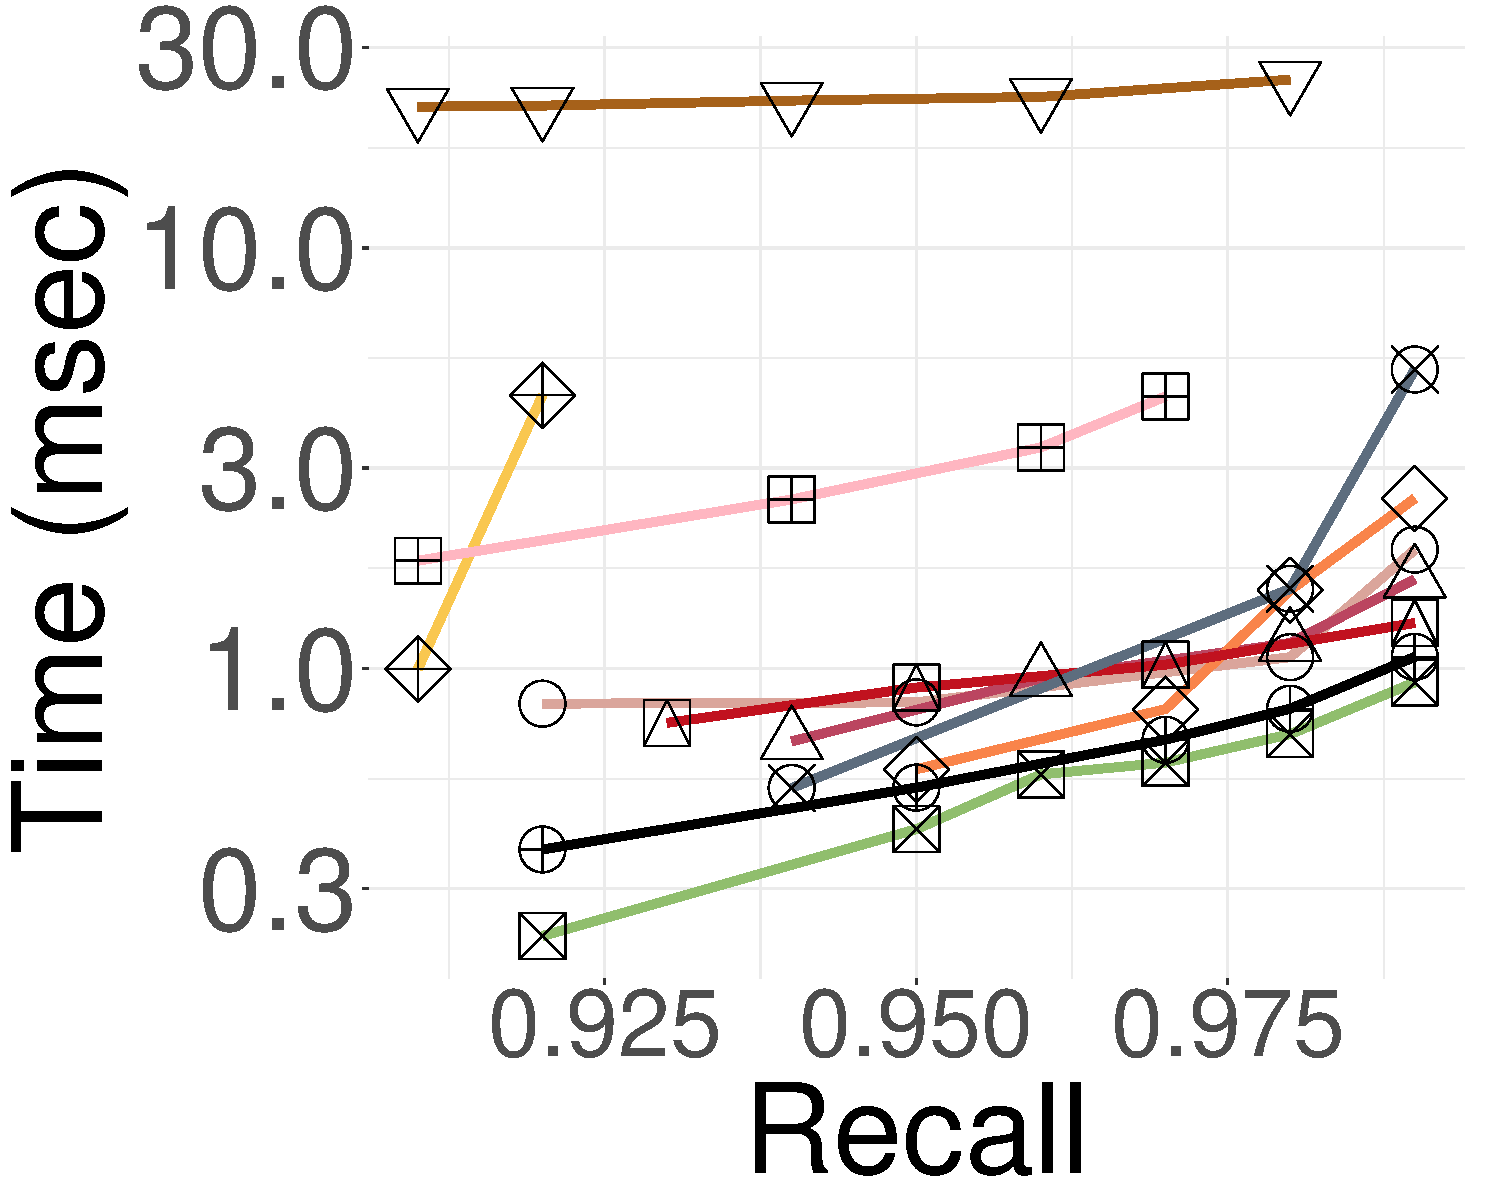
\includegraphics[width=\textwidth]{../img/Experiments/search/25/deep_10nn.pdf}
			\caption{Deep}  
		\label{fig:elpis:query:performance:25GB:deep:10NN}
		\end{subfigure}
   \hspace{0.4cm}
		\begin{subfigure}{\soneM\textwidth}
  \centering
			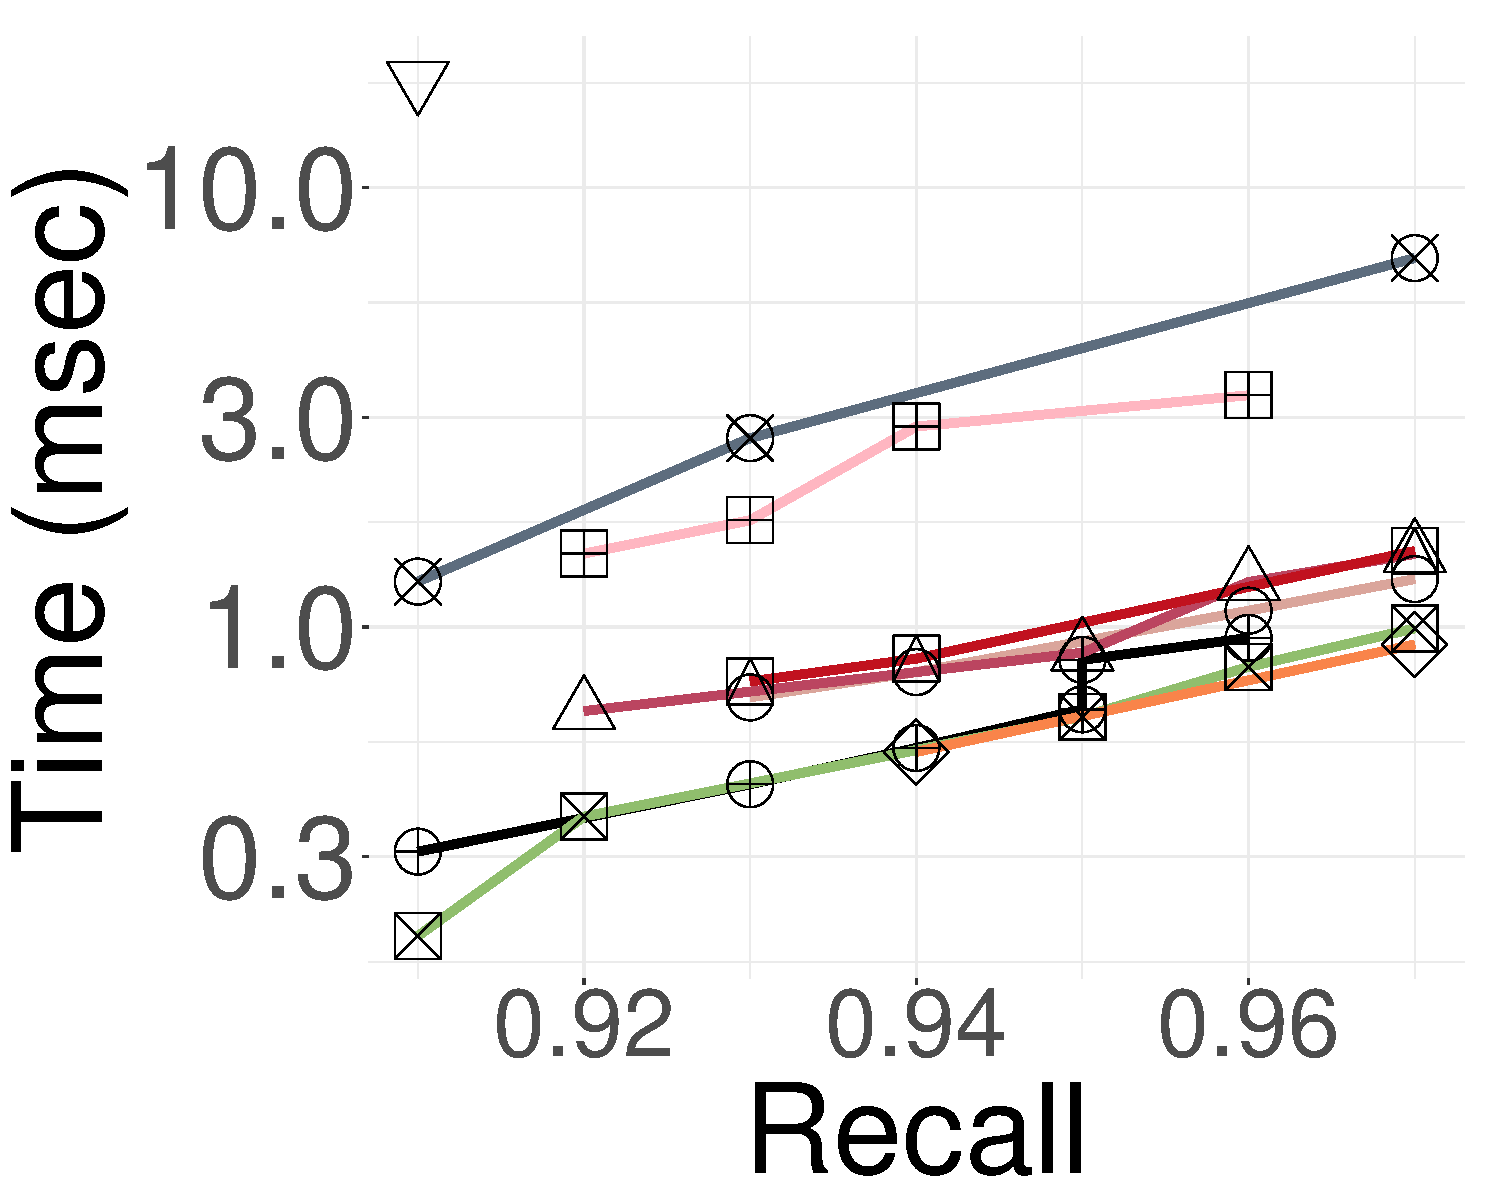
\includegraphics[width=\textwidth]{../img/Experiments/search/25/sald_10nn.pdf}
			\caption{SALD}  
		\label{fig:elpis:query:performance:25GB:sald:10NN}
		\end{subfigure}
  \hspace{0.4cm}
		\begin{subfigure}{\soneM\textwidth}
  \centering
			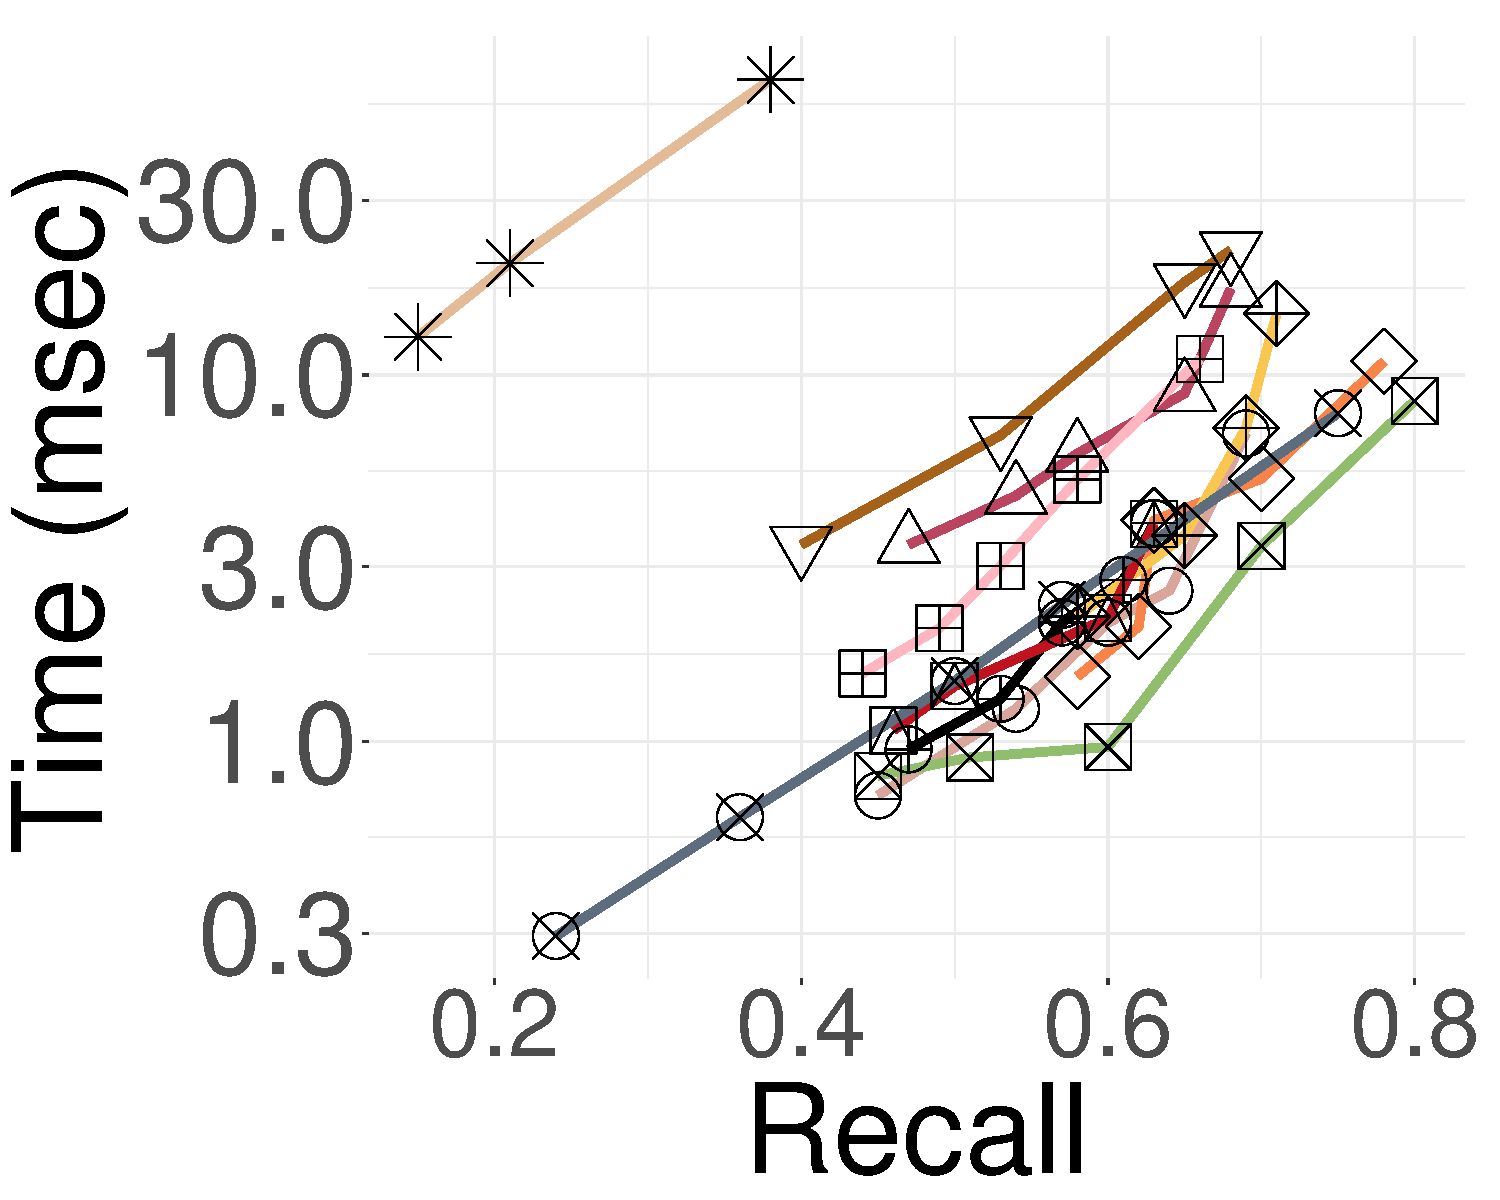
\includegraphics[width=\textwidth]{../img/Experiments/search/25/seismic_10nn.pdf}
			\caption{Seismic}  
			\label{fig:elpis:query:performance:25GB:seismic:10NN}
		\end{subfigure}	
  
		\begin{subfigure}{\soneM\textwidth}
  \centering
			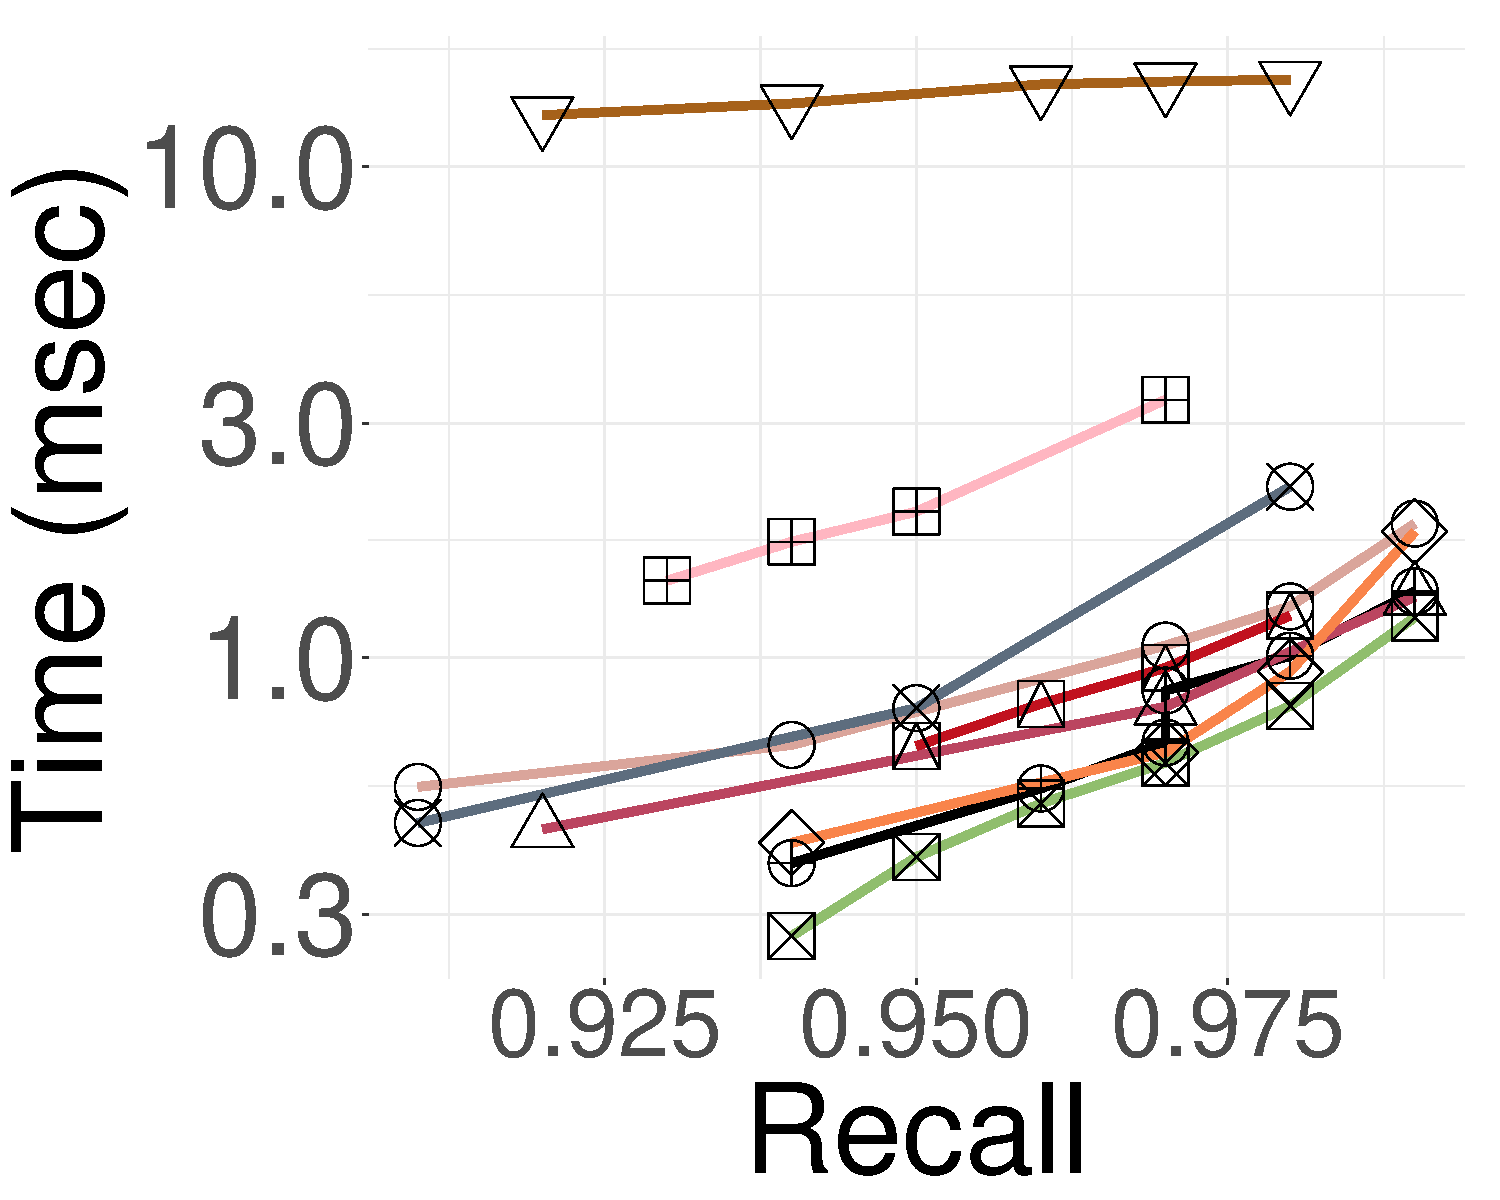
\includegraphics[width=\textwidth]{../img/Experiments/search/25/sift_10nn.pdf}
			\caption{Sift}  
			\label{fig:elpis:query:performance:25GB:sift:10NN}
		\end{subfigure}
   \hspace{0.4cm}
	\begin{subfigure}{\soneM\textwidth}
 \centering
		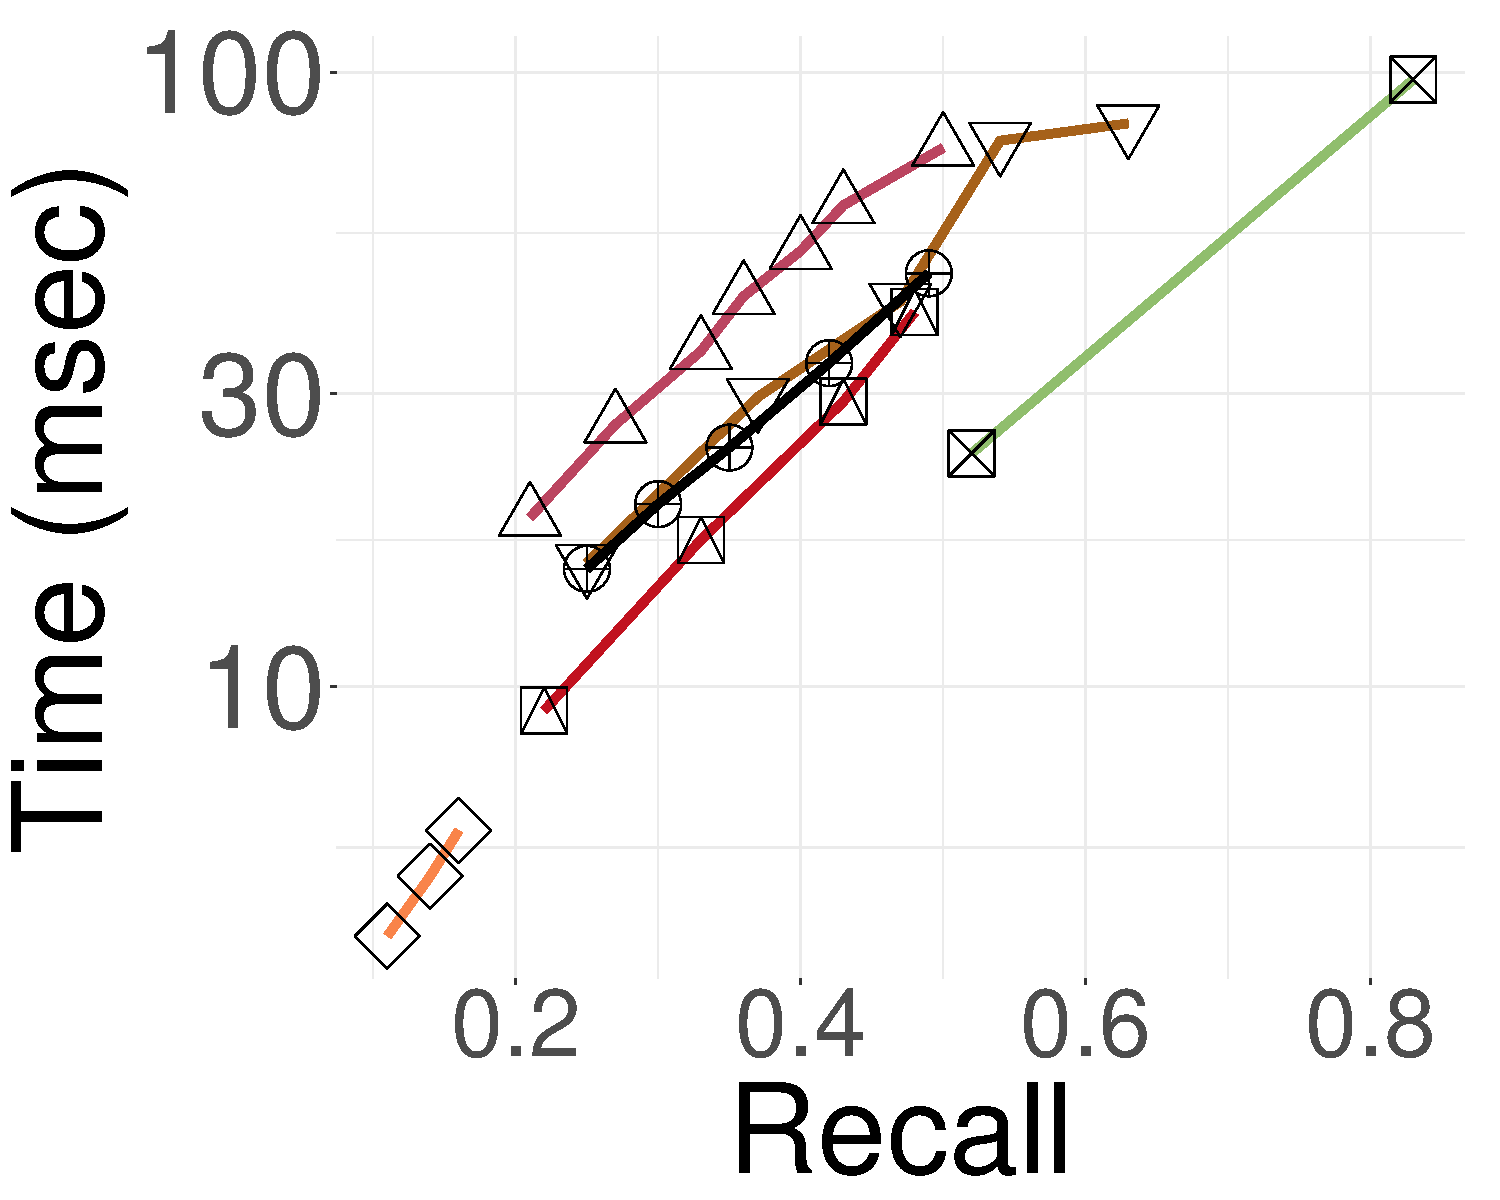
\includegraphics[width=\textwidth]{../img/Experiments/search/25/pow1_10nn.pdf}
		\caption{\textbf{RandPow0}} 
		\label{fig:query:performance:25GB:rand:pow1:10NN}
	\end{subfigure}
   \hspace{0.4cm}
	\begin{subfigure}{\soneM\textwidth}
 \centering
		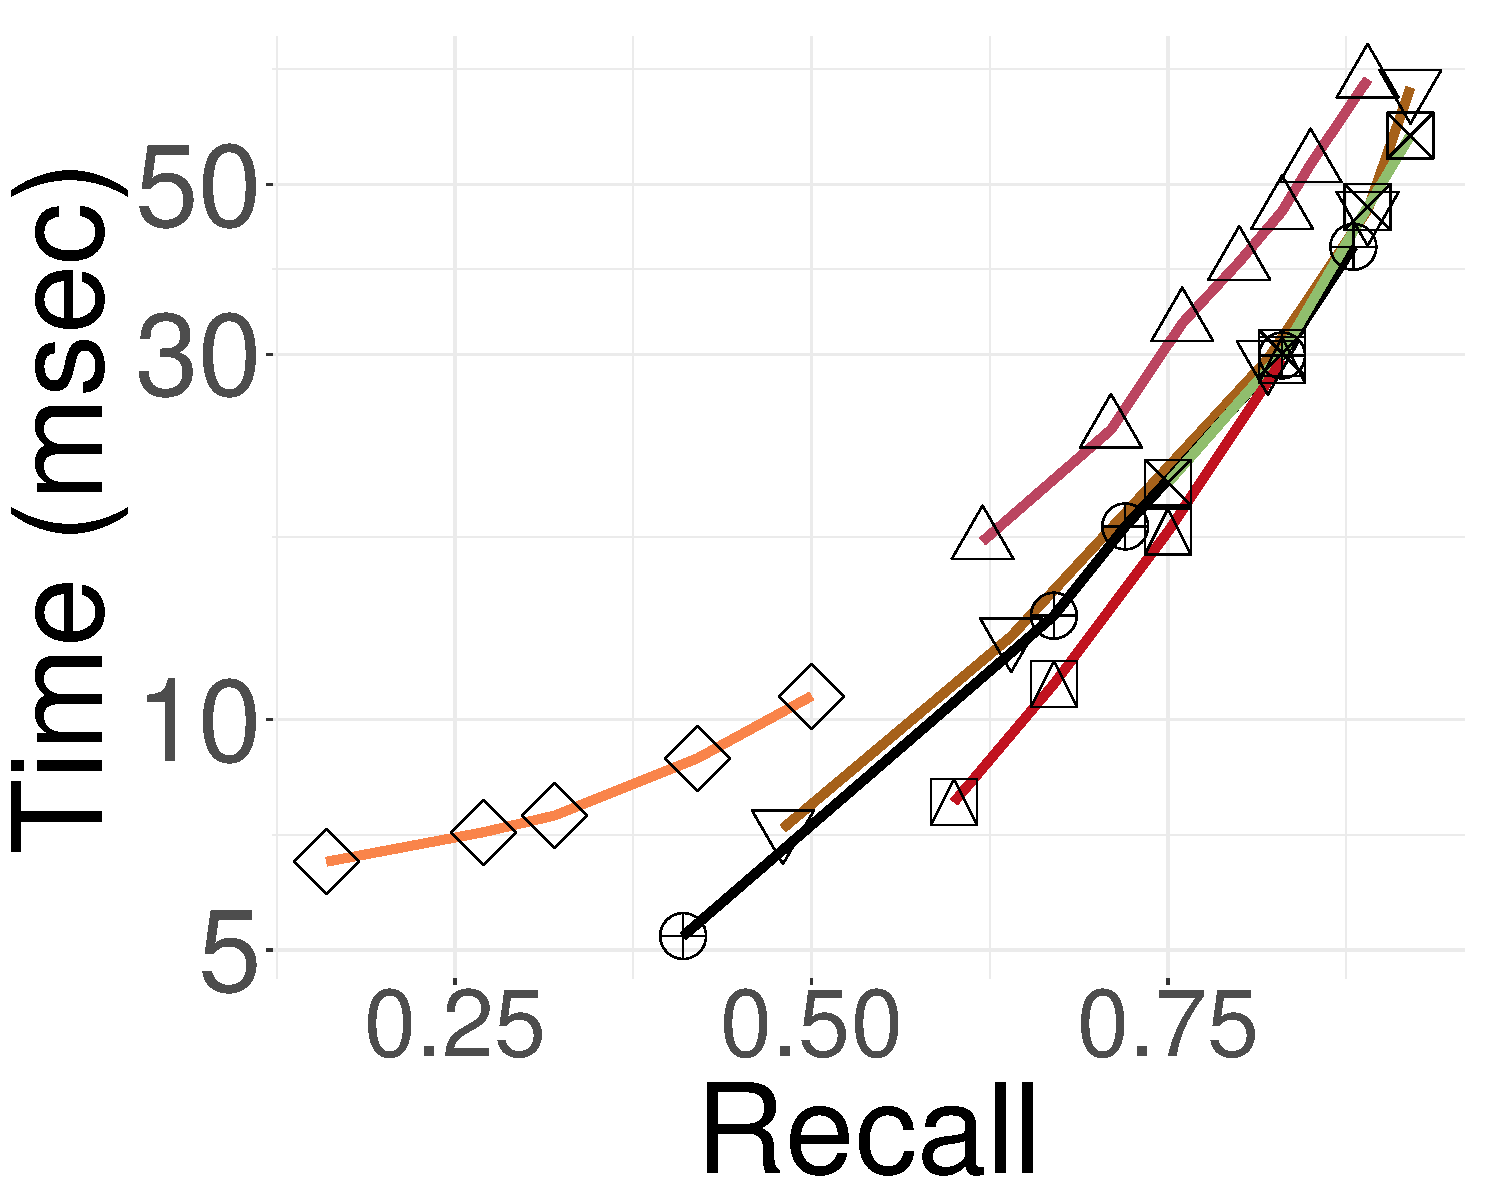
\includegraphics[width=\textwidth]{../img/Experiments/search/25/pow50_10nn.pdf}
		\caption{\textbf{RandPow50}} 
		\label{fig:query:performance:25GB:rand:pow50:10NN}
	\end{subfigure}		
		\caption{{25GB datasets}}
		\label{fig:elpis:query:performance:25GB}
	\end{minipage}
\end{figure}

\renewcommand{\soneM}{0.28}
\begin{figure}[!htb]
\captionsetup{justification=centering}
	\centering
		\begin{subfigure}{\textwidth}
			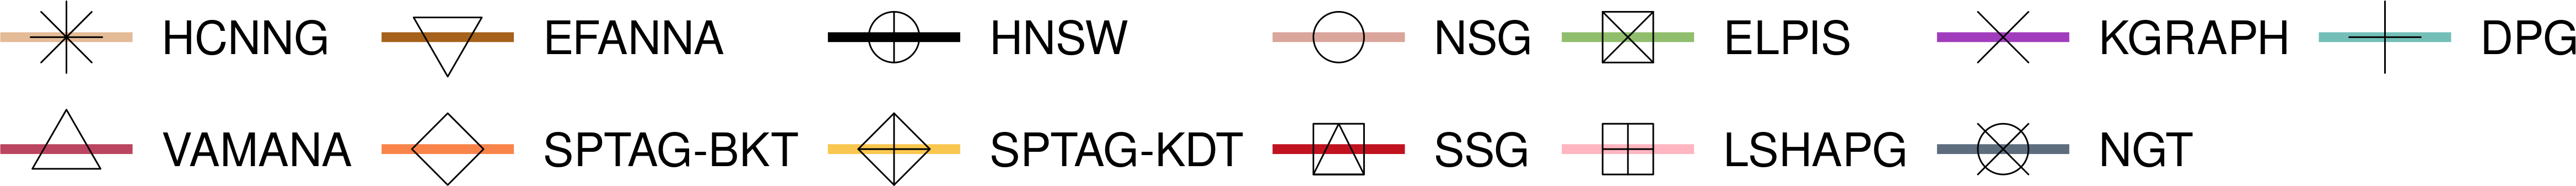
\includegraphics[width=\textwidth]{../img/Experiments/legendall.png}
		\end{subfigure}	
		\captionsetup{justification=centering}
		\captionsetup[subfigure]{justification=centering}
		\begin{subfigure}{\soneM\textwidth}
  \centering
		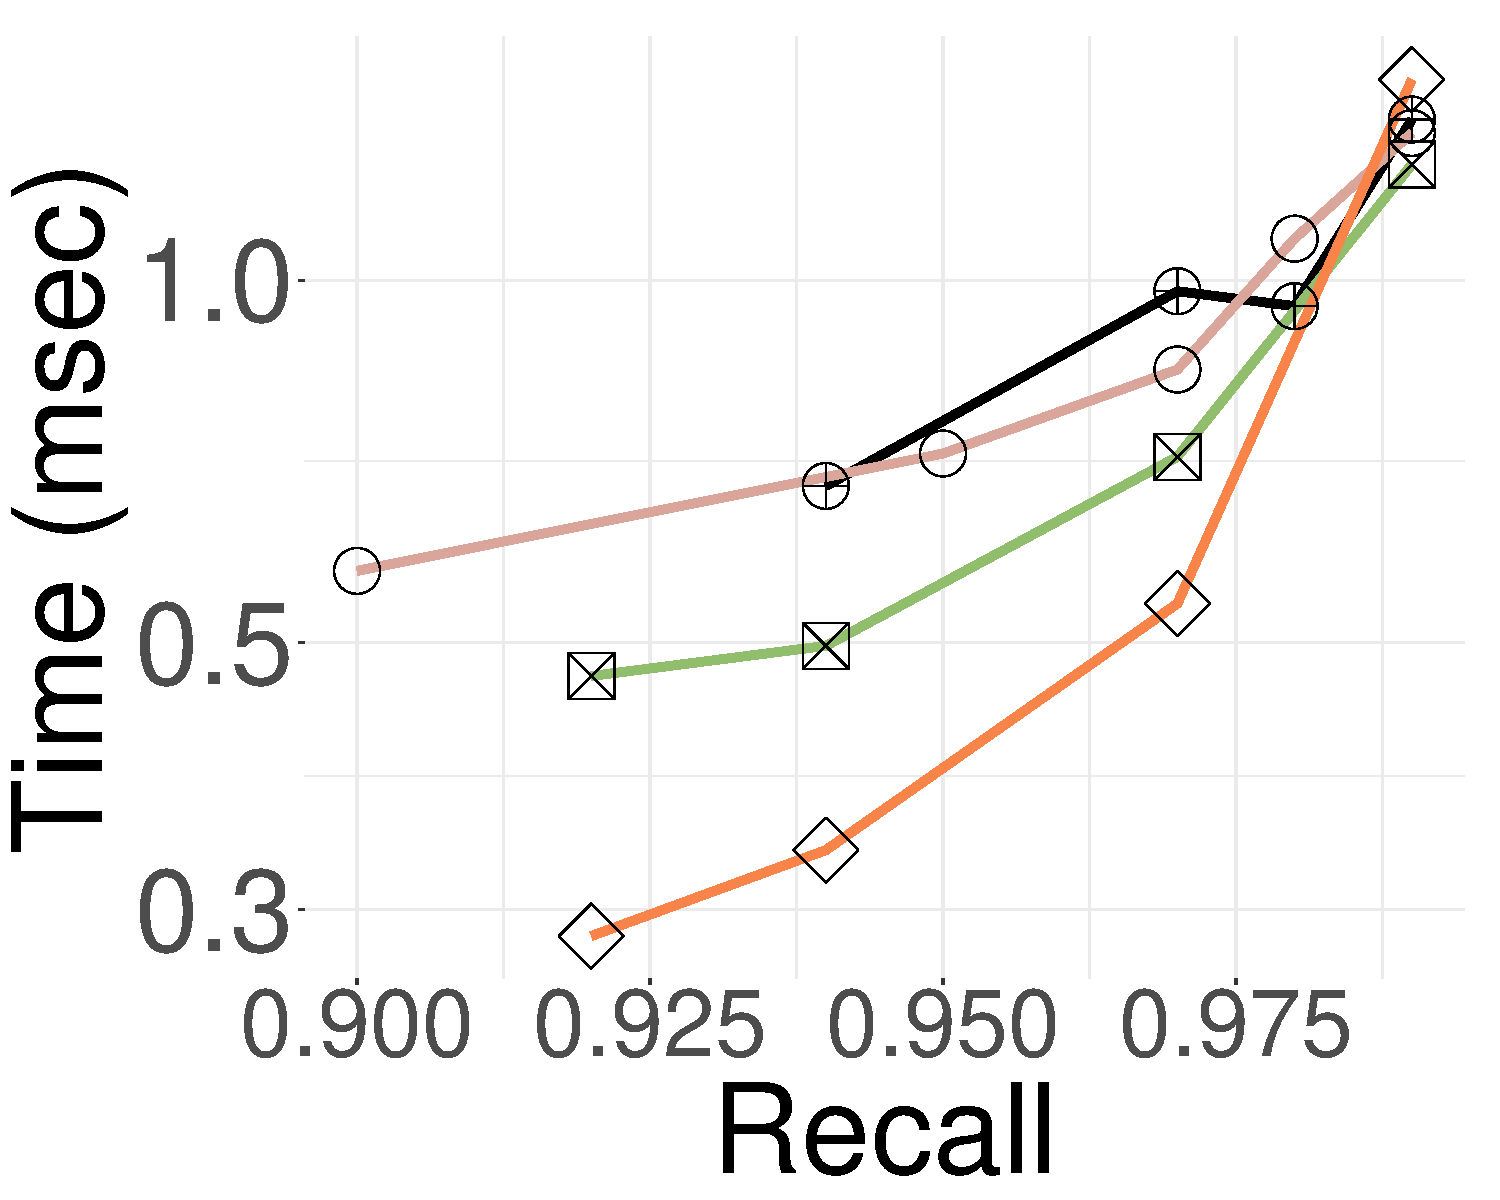
\includegraphics[width=\textwidth]{../img/Experiments/search/25/deep1p_10nn.pdf}
		\caption{\textbf{1\% noise}} 
		\label{fig:search:query:performance:25GB:hard:1p}
		\end{subfigure}
    \hspace{0.4cm}
  		\begin{subfigure}{\soneM\textwidth}
  \centering
		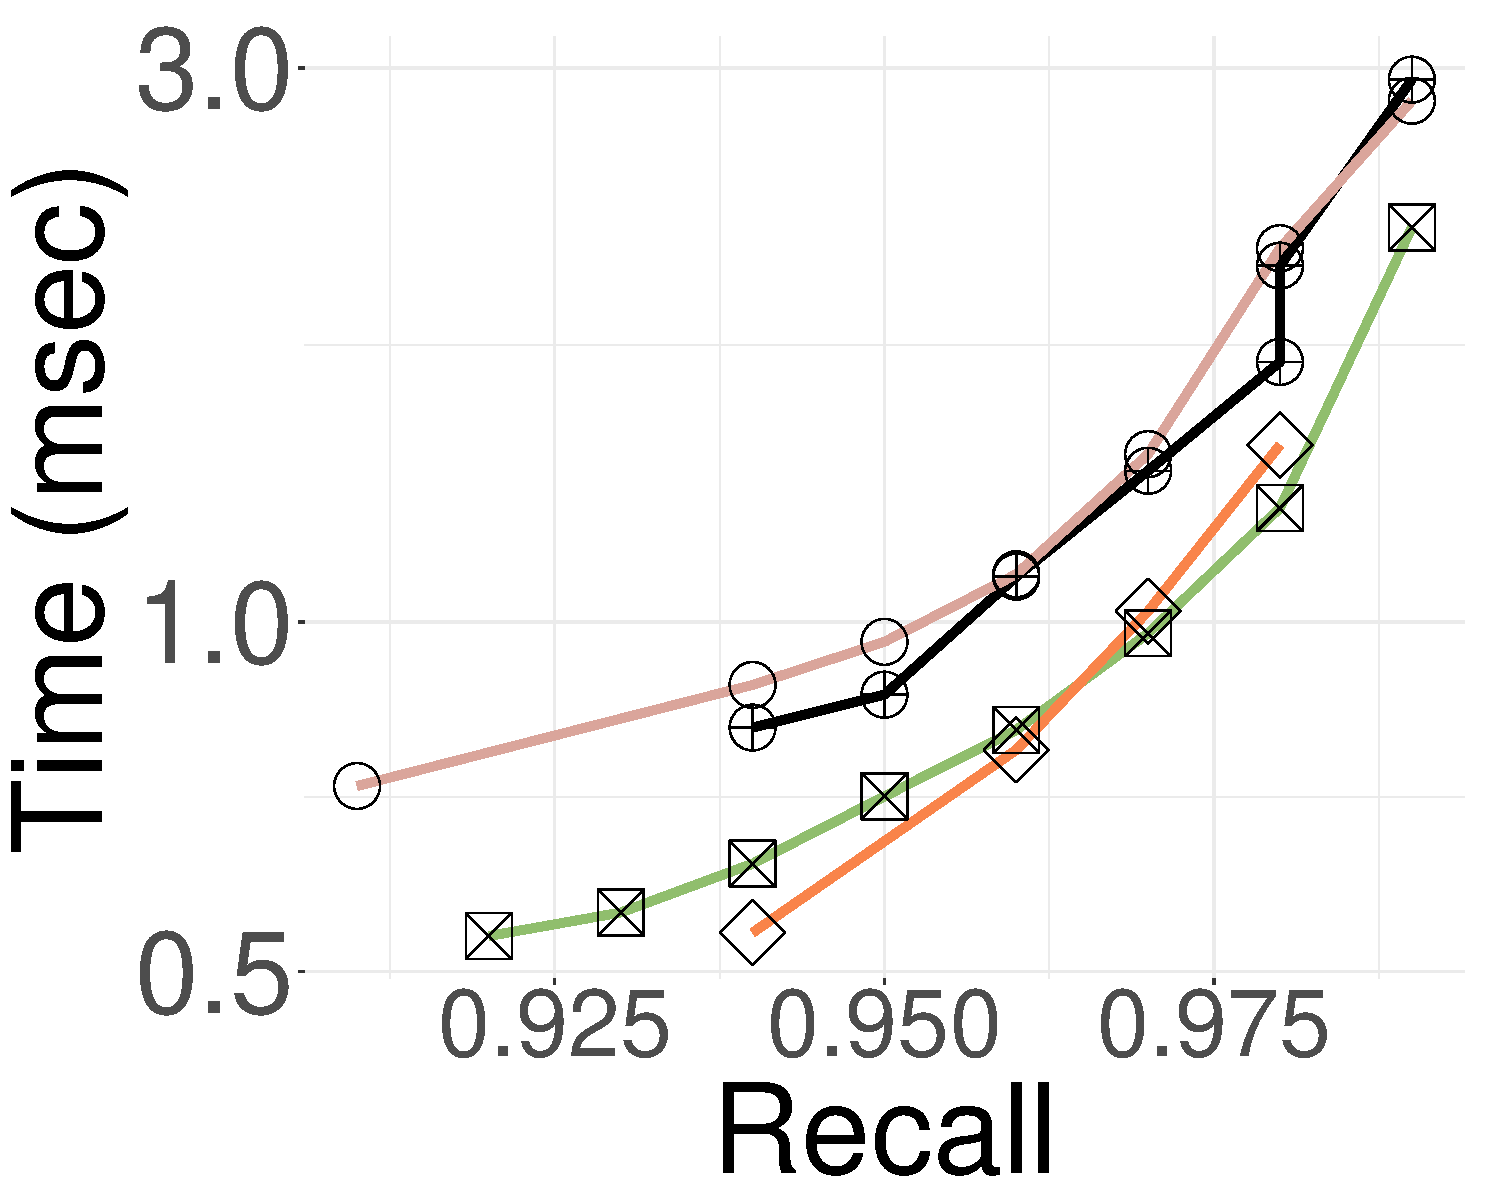
\includegraphics[width=\textwidth]{../img/Experiments/search/25/deep5p_10nn.pdf}
		\caption{\textbf{5\% noise}} 
		\label{fig:search:query:performance:25GB:hard:1p}
		\end{subfigure}
    \hspace{0.4cm}
		\begin{subfigure}{\soneM\textwidth}
  \centering
		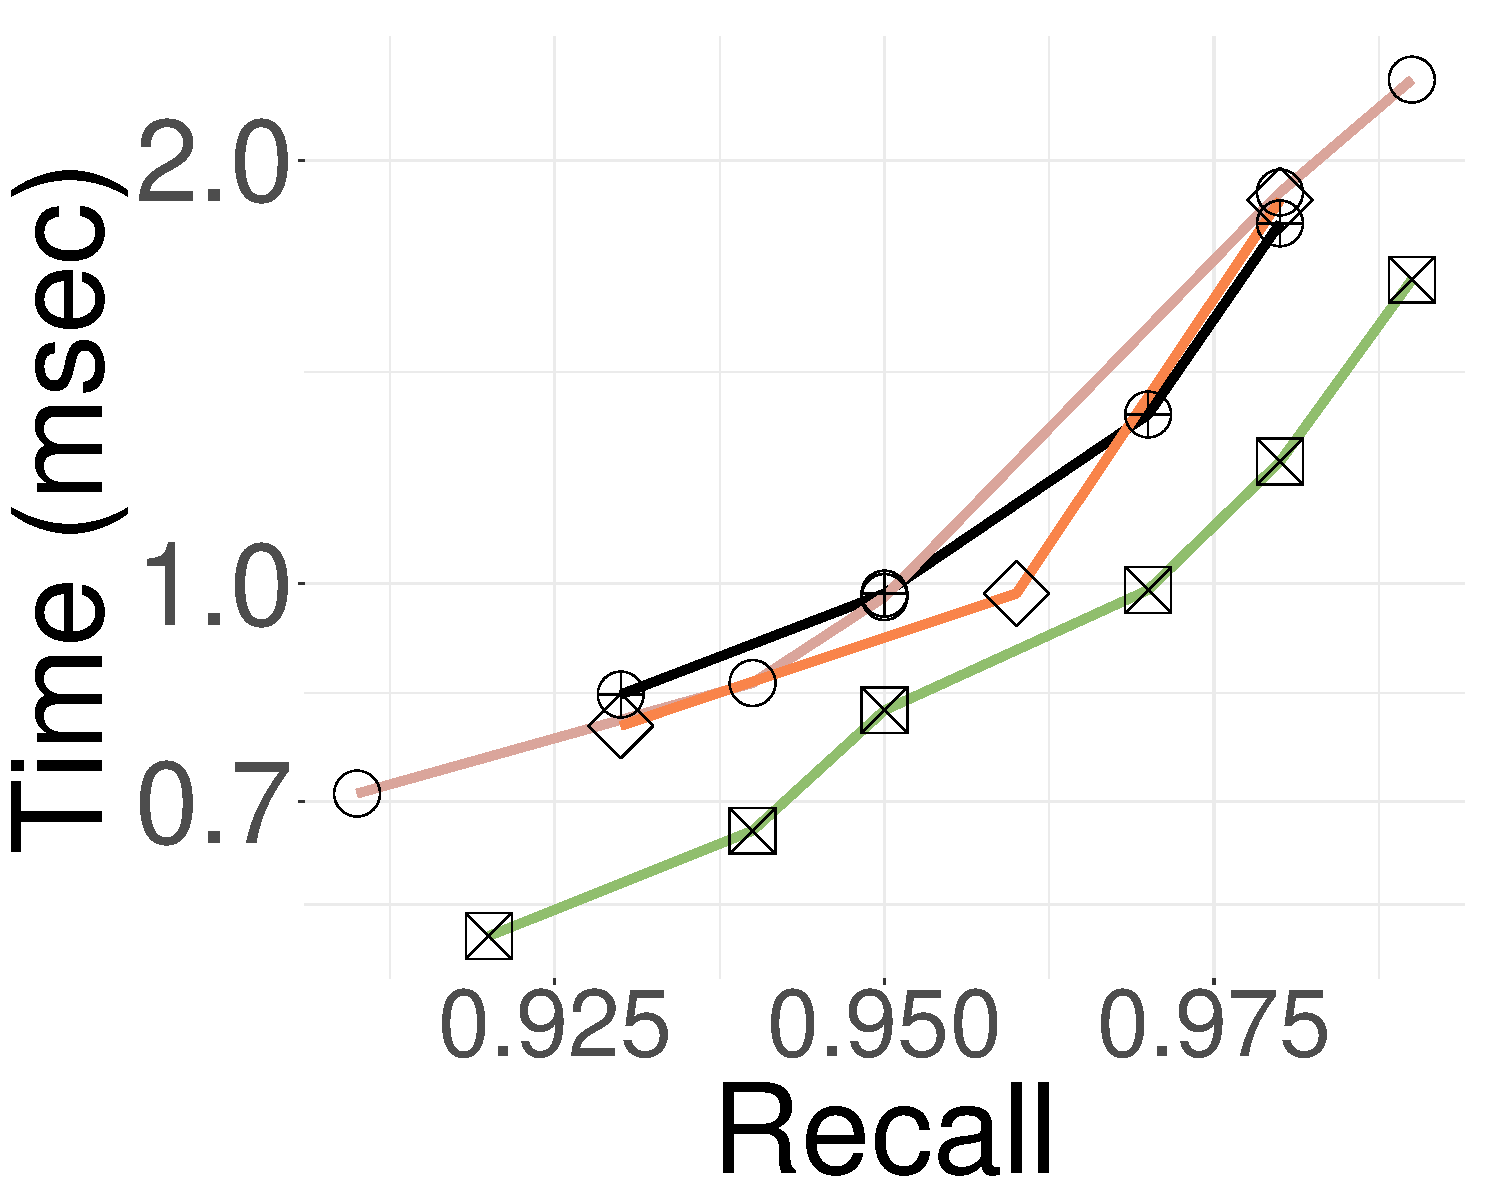
\includegraphics[width=\textwidth]{../img/Experiments/search/25/deep10p_10nn.pdf}
		\caption{\textbf{10\% noise}} 
		\label{fig:search:query:performance:25GB:hard:10p}
		\end{subfigure}
	\caption{Search Performance on Varying workloads difficulty}
		\label{fig:search:query:performance:25GB:hard}
	\end{figure}

 \begin{figure}[!htb]
		\captionsetup{justification=centering}
		\captionsetup[subfigure]{justification=centering}
  	\centering
		\begin{subfigure}{\textwidth}
			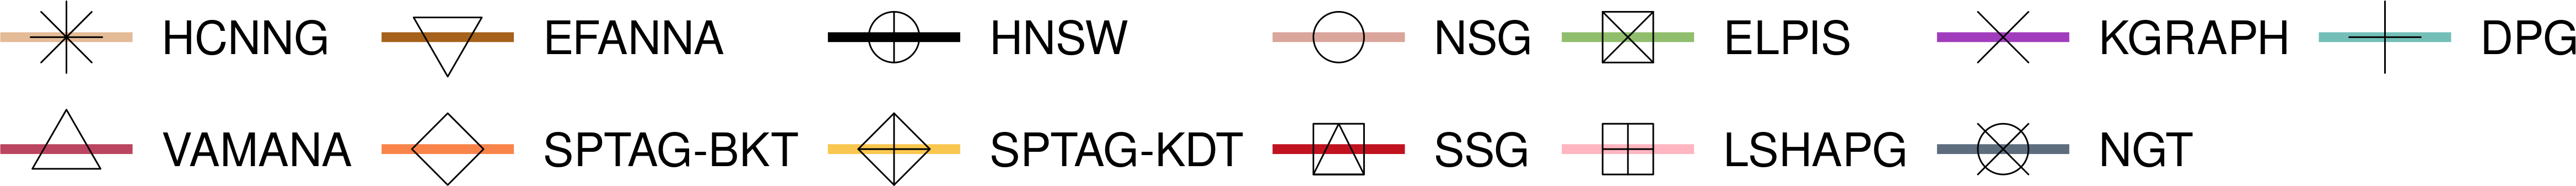
\includegraphics[width=\textwidth]{../img/Experiments/legendall.png}
		\end{subfigure}	
		\begin{subfigure}{\soneM\textwidth}
  \centering
			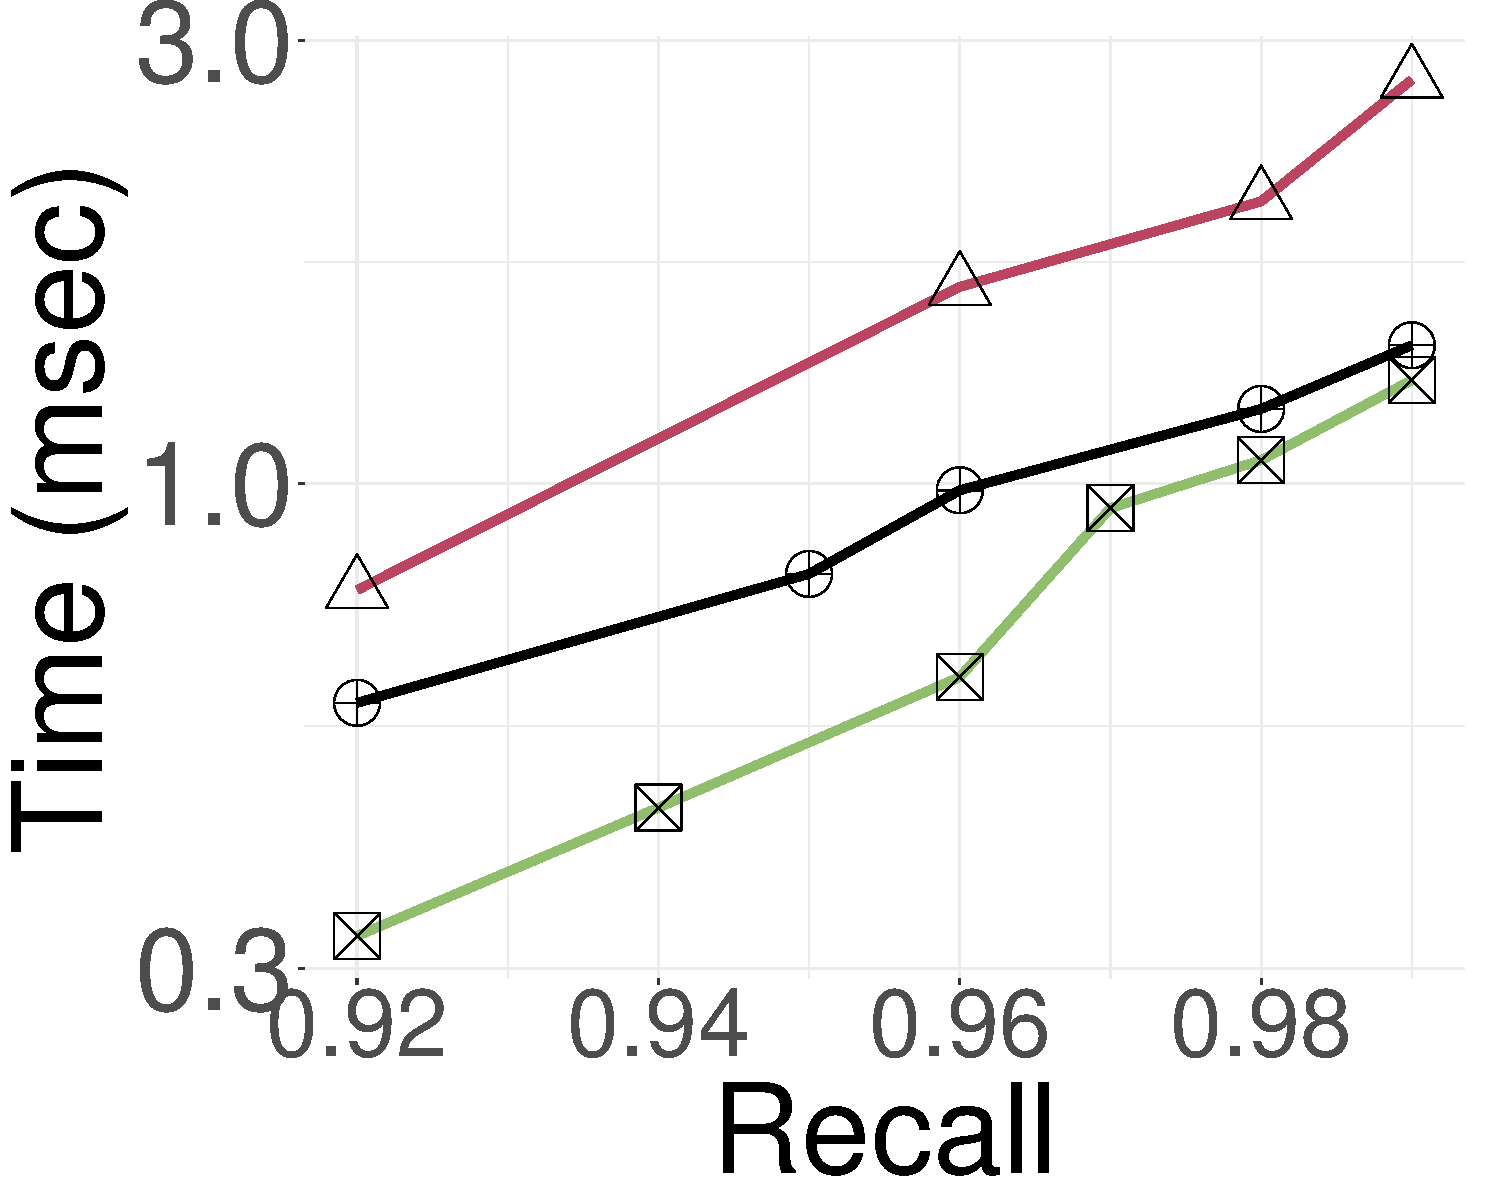
\includegraphics[width=\textwidth]{../img/Experiments/search/100/deep_10nn.pdf}
			\caption{Deep}  
		\label{fig:elpis:query:performance:100GB:deep:10NN}
		\end{subfigure}
    \hspace{0.4cm}
		\begin{subfigure}{\soneM\textwidth}
  \centering
			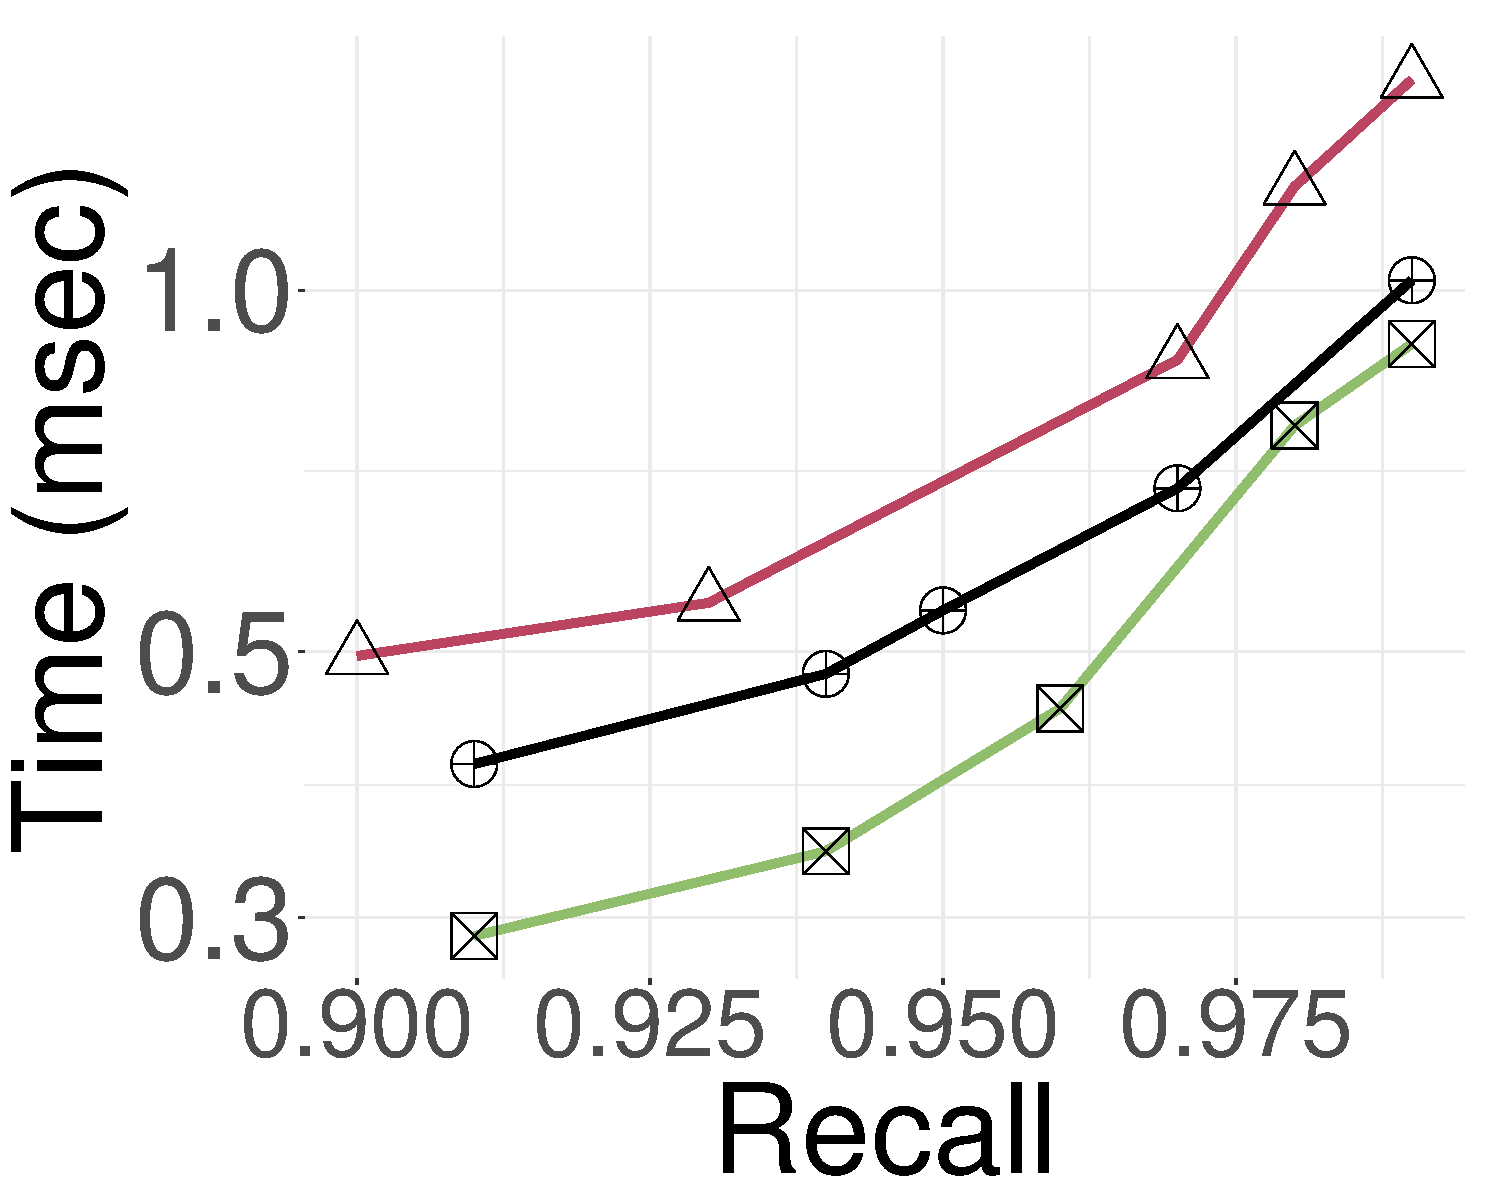
\includegraphics[width=\textwidth]{../img/Experiments/search/100/sift_10nn.pdf}
			\caption{Sift}  
		\label{fig:elpis:query:performance:100GB:sift:10NN}
		\end{subfigure}
    \hspace{0.4cm}
  		\begin{subfigure}{\soneM\textwidth}
  \centering
			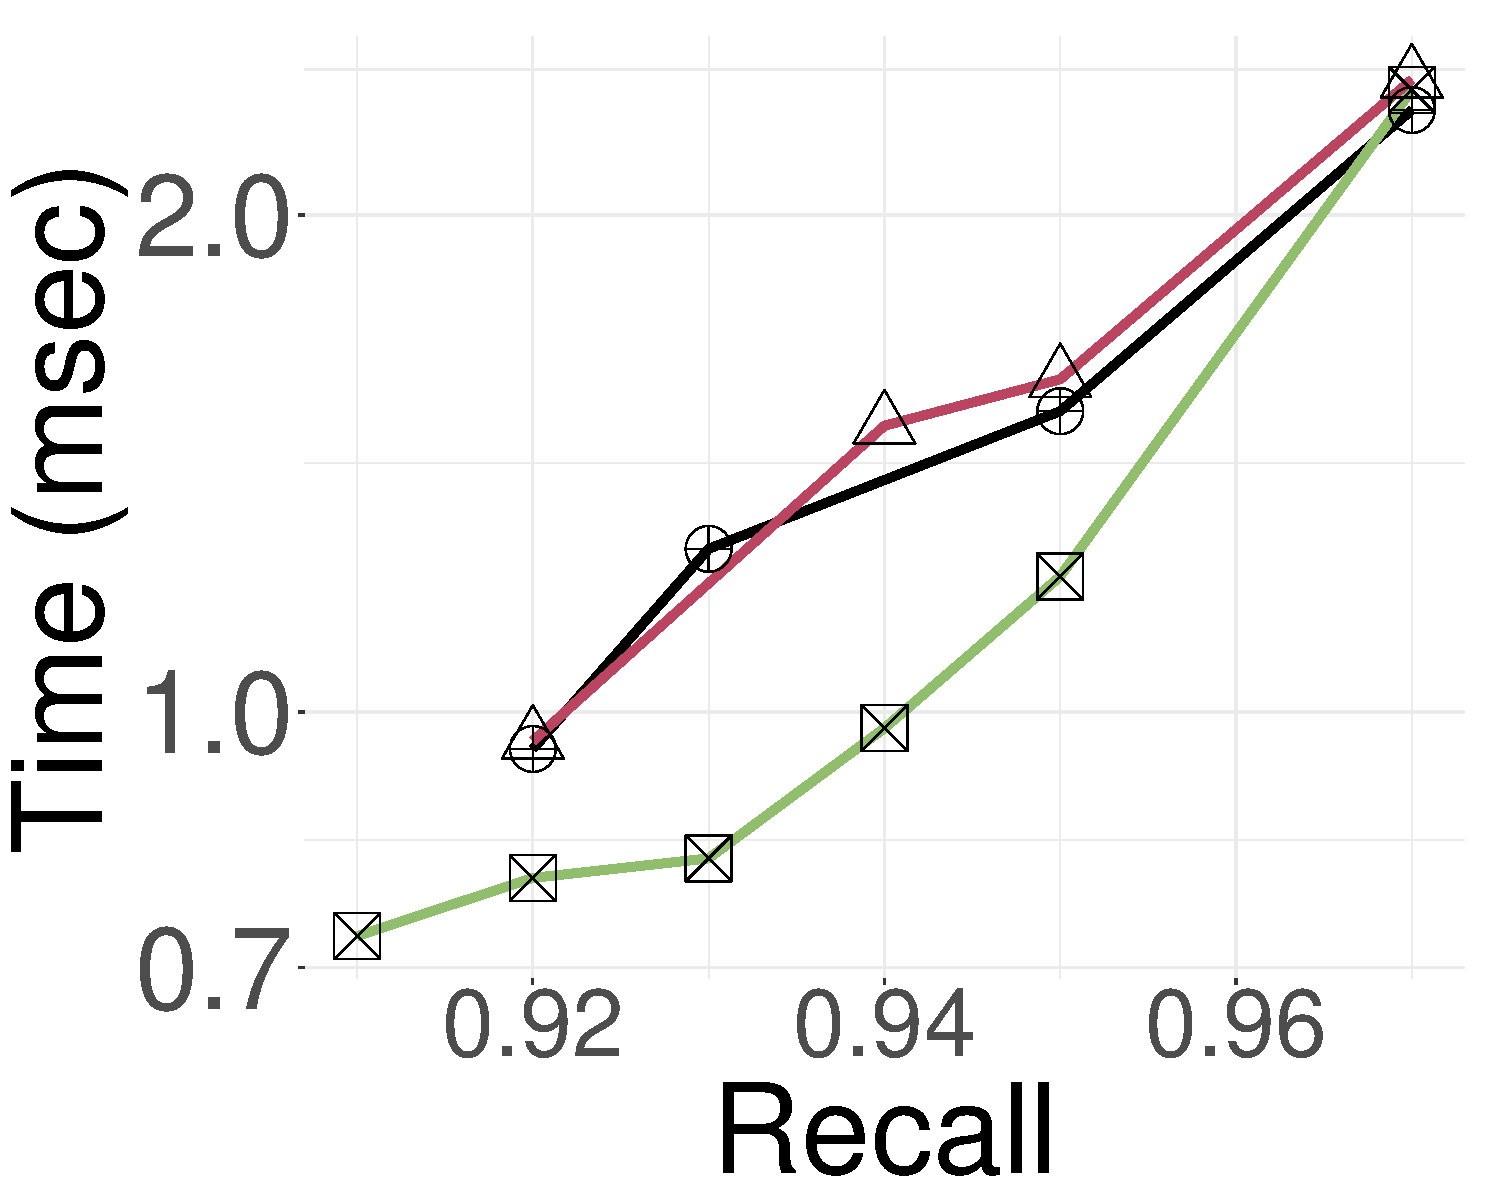
\includegraphics[width=\textwidth]{../img/Experiments/search/100/sald_10nn.pdf}
			\caption{Sald}  
		\label{fig:elpis:query:performance:100GB:sald:10NN}
		\end{subfigure}
		\caption{{Search Performance on 100GB datasets}}	
		\label{fig:elpis:query:performance:100GB}
	\end{figure}
 
	\begin{figure}
		\captionsetup{justification=centering}
		\captionsetup[subfigure]{justification=centering}
  	\centering
		\begin{subfigure}{\textwidth}
			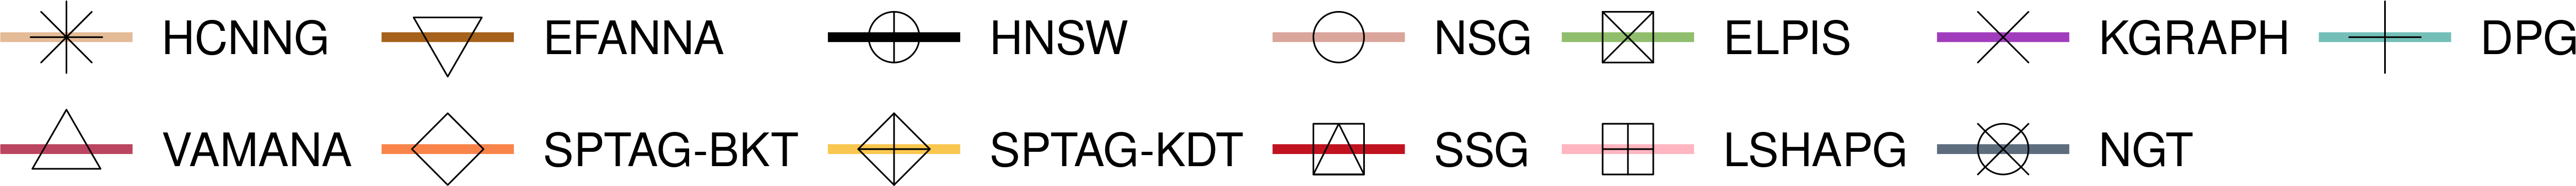
\includegraphics[width=\textwidth]{../img/Experiments/legendall.png}
		\end{subfigure}	
		\begin{subfigure}{\soneM\textwidth}
			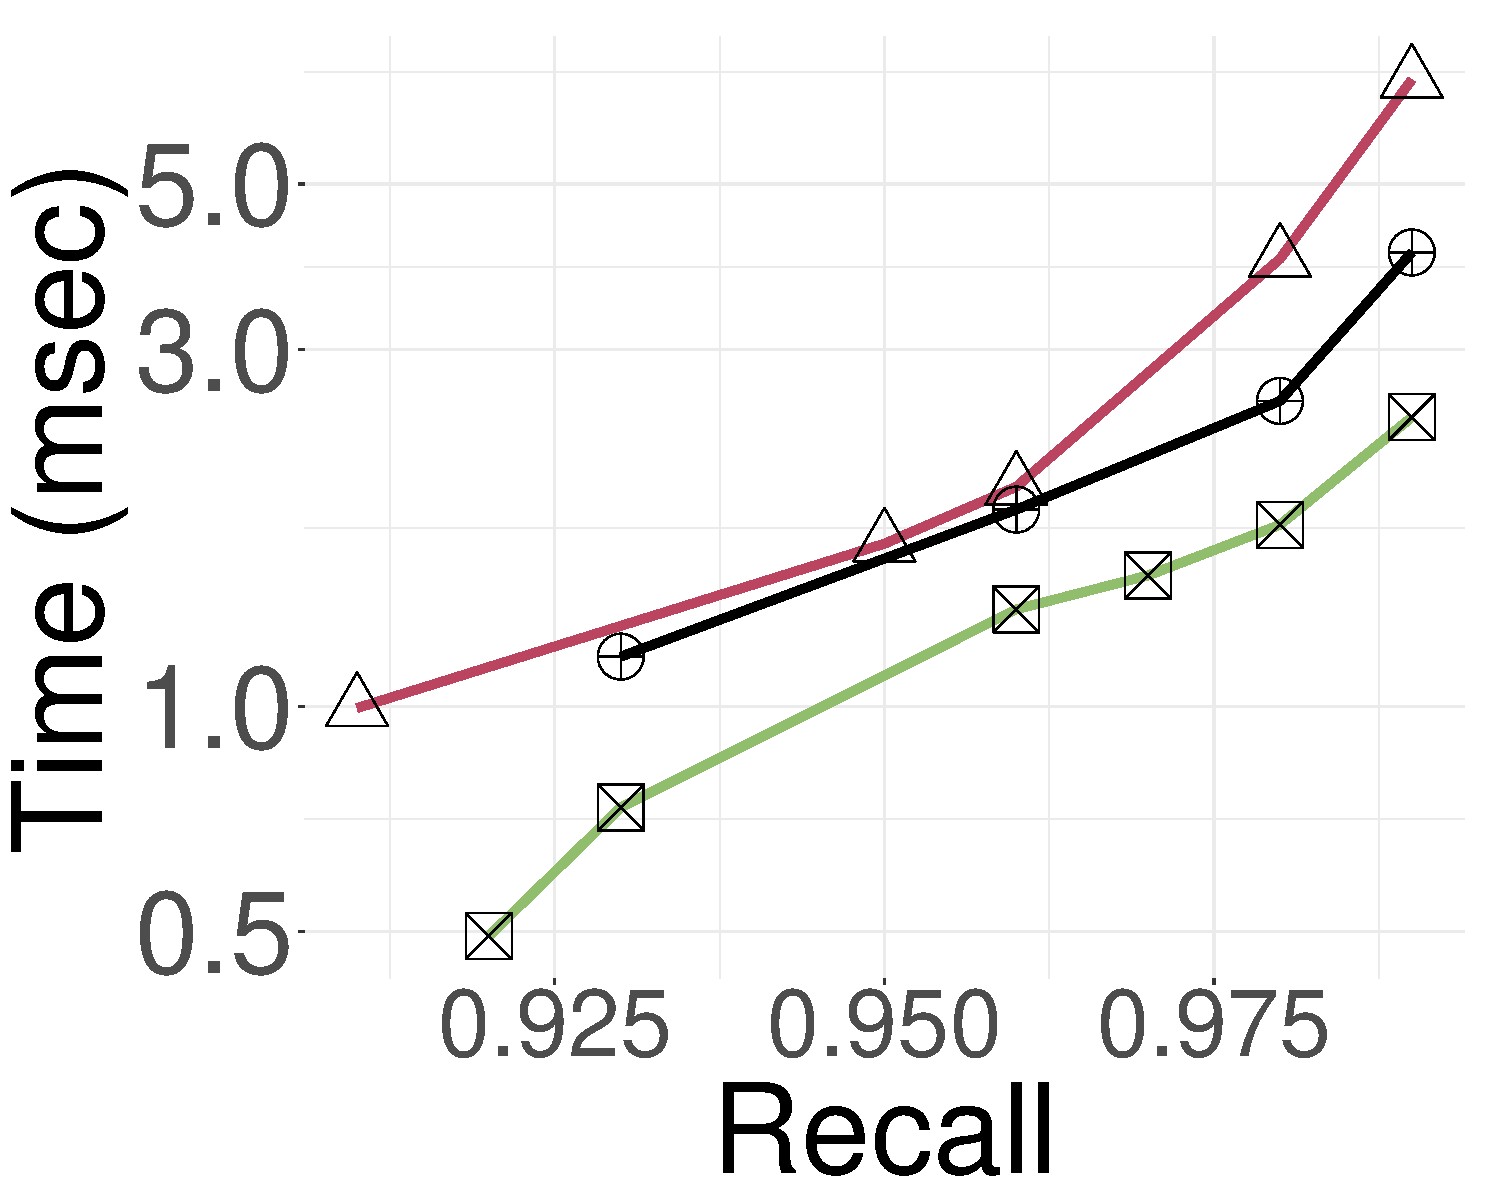
\includegraphics[width=\textwidth]{../img/Experiments/search/1B/deep_10nn.pdf}
			\caption{Deep}  
		\label{fig:elpis:query:performance:1B:deep:10NN}
		\end{subfigure}
    \hspace{0.4cm}
		\begin{subfigure}{\soneM\textwidth}
			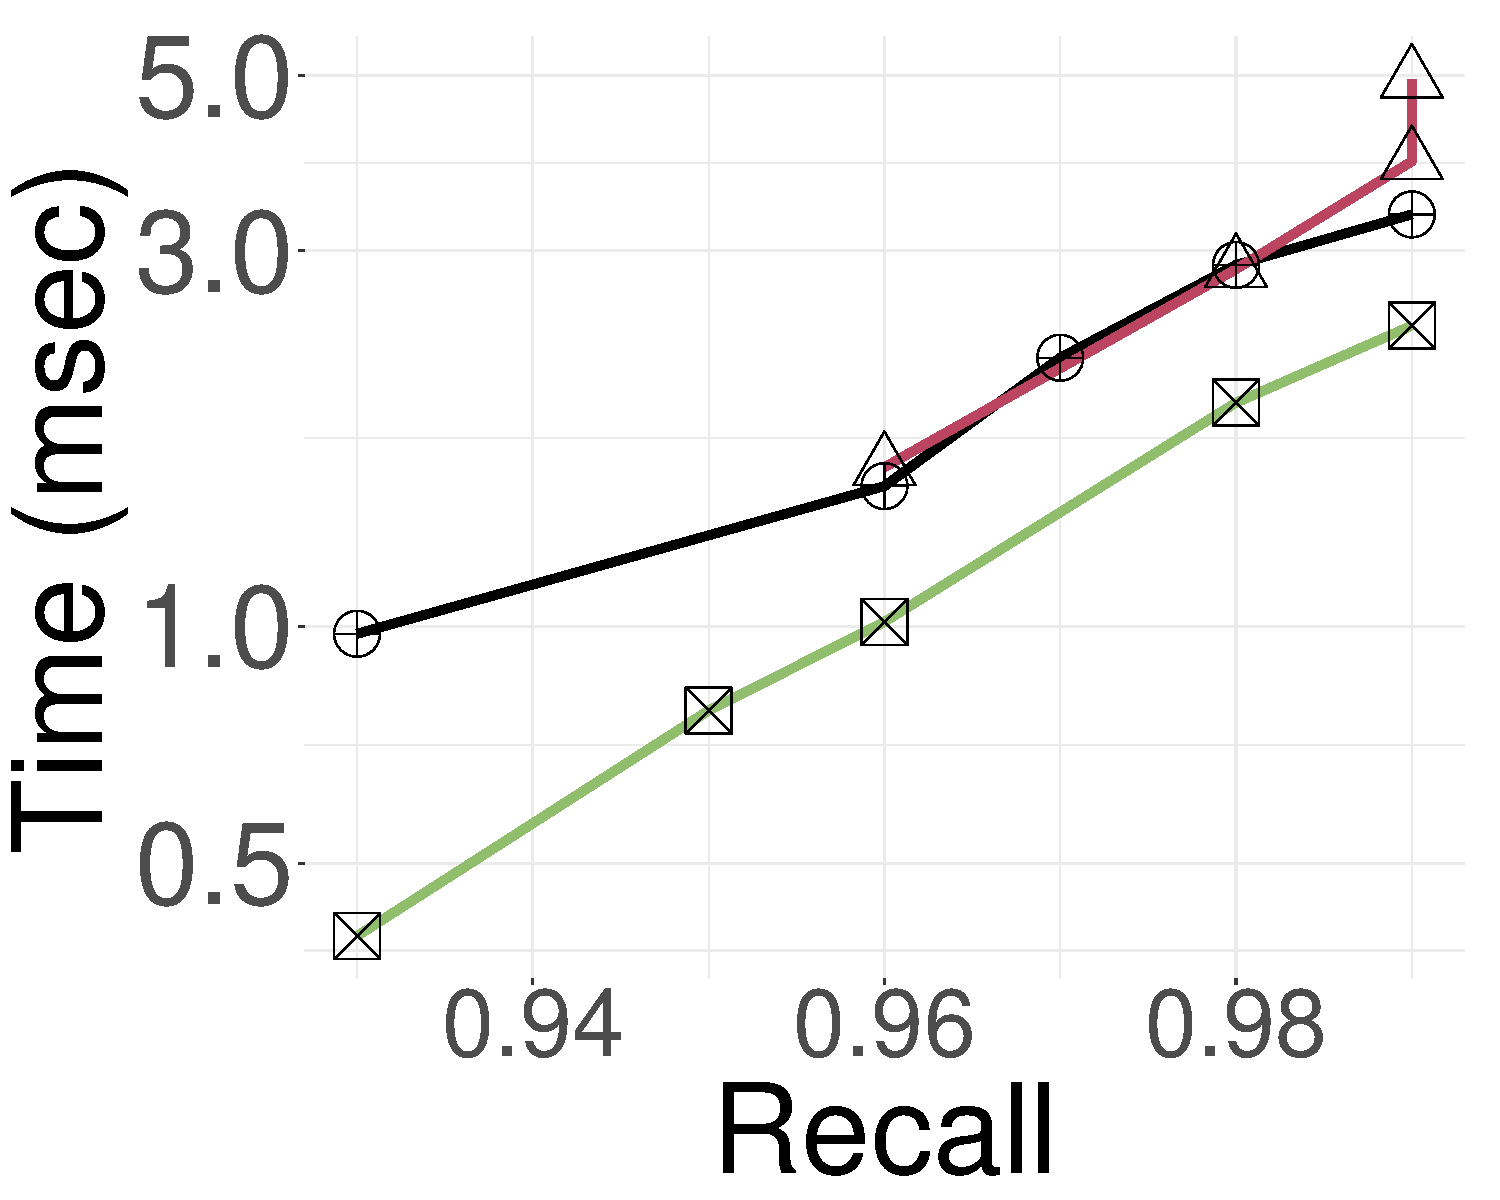
\includegraphics[width=\textwidth]{../img/Experiments/search/1B/sift_10nn.pdf}
			\caption{Sift}  
			\label{fig:elpis:query:performance:1B:sift:10NN}
		\end{subfigure}
    \hspace{0.4cm}
  		\begin{subfigure}{\soneM\textwidth}
			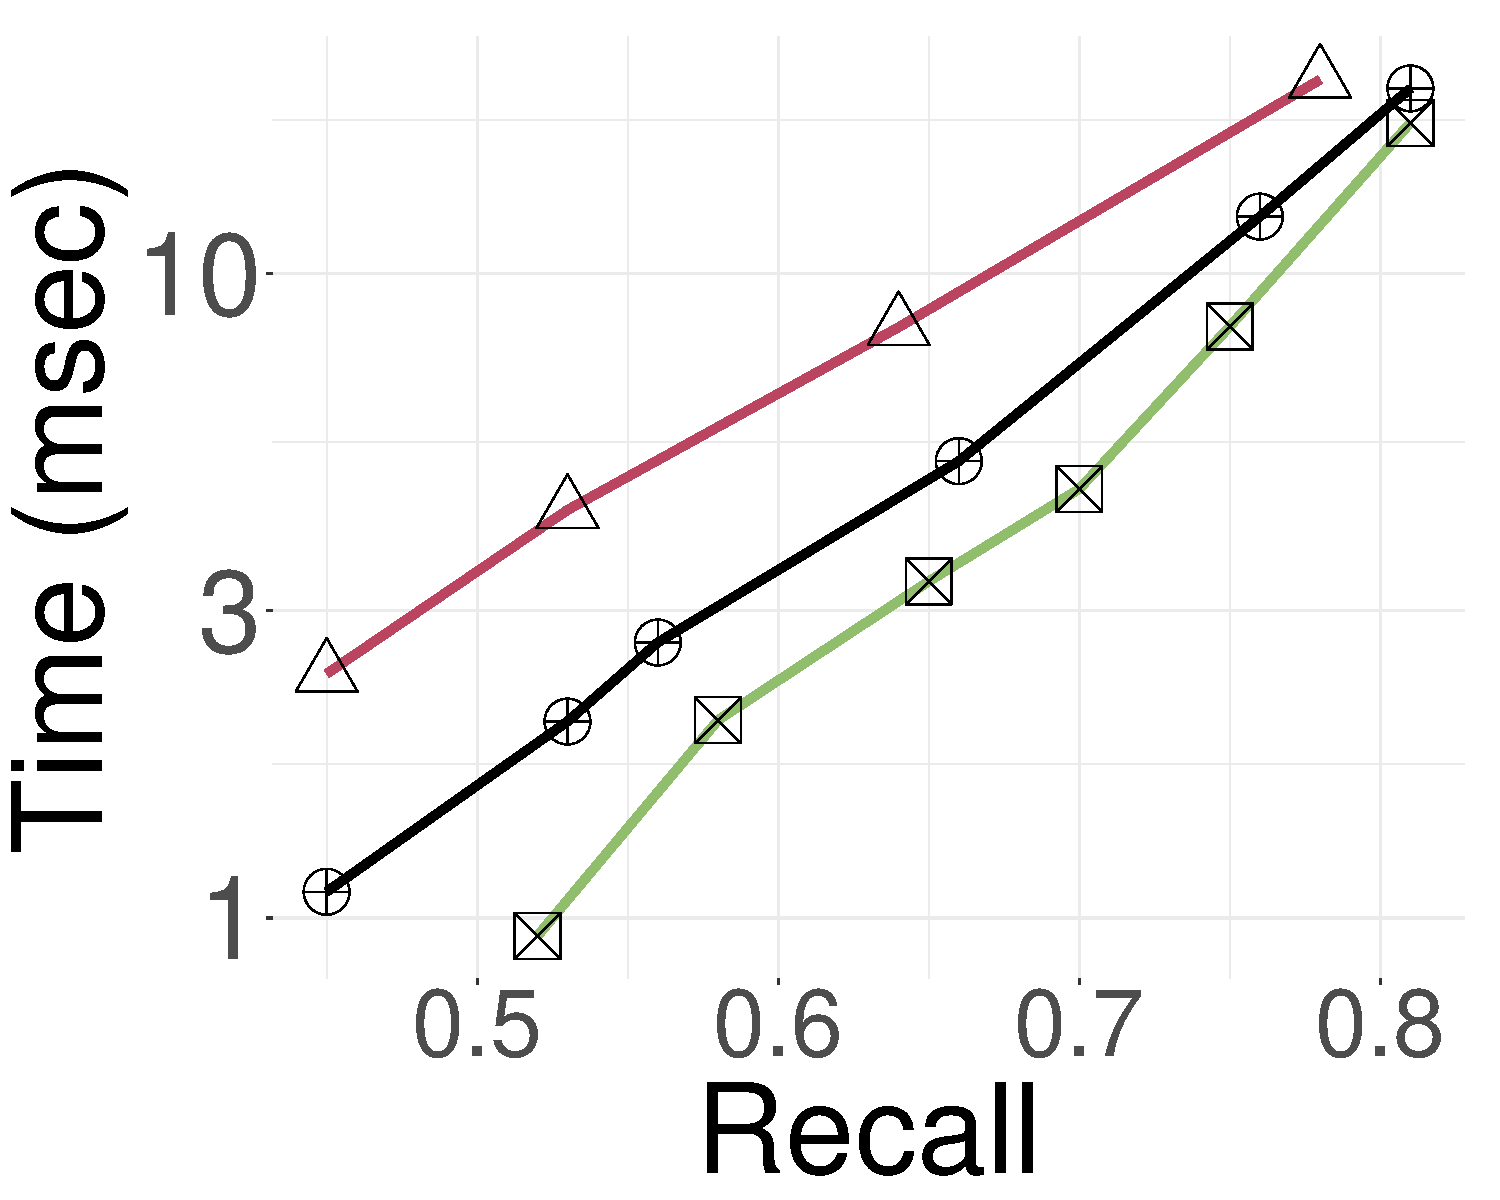
\includegraphics[width=\textwidth]{../img/Experiments/search/1B/text2img_10nn.pdf}
			\caption{Text-to-Image}  
			\label{fig:elpis:query:performance:1B:t2i:10NN}
		\end{subfigure}
		\caption{{Search Performance on 1B datasets}}	
		\label{fig:elpis:query:performance:1B}
	\end{figure}

\section{Discussion}
\label{sec:discussion}
In the previous section, we reported the results of our extensive experimental evaluation
of ten state-of-the-art graph-based vector search methods, including ELPIS.
Table~\ref{tab:comp} summarizes the evaluation across key criteria: % for both search and indexing. 
for search, we assess efficiency, accuracy, and the number of tunable parameters; 
for indexing, we evaluate efficiency at high recall, memory footprint, and parameter tuning complexity. 

The best-performing methods, HNSW, VAMANA, and ELPIS, have the best search performance and index efficiency. However, ELPIS requires an extra parameter during both indexing (leaf size) and search (nprobes), whereas VAMANA requires an extra parameter to tune during indexing (alpha). NSG and SSG exhibit efficient query performance, but their indexing capability is hindered because of their base graph EFANNA, which similarly to KGraph, is tedious to tune and suffers from high indexing time and footprint. Both SPTAG (BKT) and NGT show satisfactory performance during search; however, they do not scale well to large datasets and require more tuning compared to the best methods. The assessment of HCCNG is based on the optimized parlayNN implementation which has shown competitive performance on large-scale datasets~\cite{parlayann}.

\begin{table}[ht]
\begin{minipage}{0.8\textwidth}
\hspace{3.5cm}
$\checkmark$ Good \quad
$\sim$ Medium \quad
$\times$ Bad
\end{minipage} \\[2pt]
\captionsetup{justification=centering}
\resizebox{\columnwidth}{!}{
\begin{tabular}{lccc|ccc}
\toprule
\textbf{Method} & \multicolumn{3}{c|}{\textbf{Query Answering}} & \multicolumn{3}{c}{\textbf{Index Building}} \\
                & \textbf{Efficiency} & \textbf{Accuracy} & \textbf{Tuning} & \textbf{Efficiency} & \textbf{Footprint} & \textbf{Tuning} \\
\midrule
HNSW     & $\checkmark$ & $\checkmark$ & $\checkmark$ & $\checkmark$ & $\checkmark$ & $\checkmark$ \\
ELPIS    & $\checkmark$ & $\checkmark$ & $\sim$       & $\checkmark$ & $\checkmark$ & $\sim$ \\
VAMANA   & $\checkmark$ & $\checkmark$ & $\checkmark$ & $\checkmark$ & $\checkmark$ & $\sim$ \\
NSG      & $\checkmark$ & $\checkmark$ & $\checkmark$ & $\sim$       & $\sim$       & $\sim$ \\
SSG      & $\checkmark$ & $\checkmark$ & $\checkmark$ & $\sim$       & $\sim$       & $\sim$ \\
EFANNA   & $\times$     & $\sim$       & $\times$     & $\times$     & $\times$     & $\times$ \\
KGRAPH   & $\times$     & $\times$     & $\times$     & $\times$     & $\times$     & $\times$ \\
DPG      & $\times$     & $\sim$       & $\sim$       & $\sim$       & $\sim$       & $\sim$ \\
SPTAG    & $\checkmark$       & $\checkmark$ & $\times$     & $\times$     & $\checkmark$ & $\times$ \\
HCNNG    & $\checkmark$ & $\checkmark$ & $\checkmark$ & $\checkmark$ & $\checkmark$ & $\sim$ \\
LSHAPG   & $\times$     & $\sim$       & $\times$     & $\sim$       & $\checkmark$ & $\checkmark$ \\
NGT      & $\checkmark$       & $\checkmark$       & $\times$     & $\sim$       & $\checkmark$ & $\times$ \\
\bottomrule
\end{tabular}

}
\centering
\caption{Comparative analysis}
	%\vspace*{-0.4cm}
\label{tab:comp}
\end{table}


We now summarize the key insights from both experiments, focusing on state-of-the-art approaches and different key components of graph methods, i.e., Seed Selection and Neighborhood Diversification.

\noindent{\bf Unexpected Results.} Our results reveal some interesting observations that warrant further investigation. 
\textit{(1) Stacked NSW:} while hierarchical layers of NSW graphs have shown promise in improving search performance on billion-scale datasets (Figure~\ref{fig:ss:search}), our experiments demonstrate that a simpler approach like K-random sampling can achieve better results on smaller and medium-sized datasets. 

\textit{(2) Scalability of Graph Approaches:} While all graph-based vector search methods can efficiently build indexes on small datasets, most approaches face significant scalability challenges. Some methods (SPTAG-BKT, NSG, and SSG) demonstrate impressive search performance on 1M and 25GB datasets (Figs.~\ref{fig:elpis:query:performance:1M:sift:10NN},~\ref{fig:elpis:query:performance:1M:deep:10NN},~\ref{fig:elpis:query:performance:25GB:seismic:10NN},~\ref{fig:elpis:query:performance:25GB:deep:10NN}, and~\ref{fig:elpis:query:performance:25GB:sald:10NN}) but their index construction could not scale to 100GB and billion-scale datasets. An important research direction is to improve the indexing scalability for these methods, either by adopting summarization techniques during index construction or by using a scalable data structure to construct the base graph (i.e., IVFPQ~\cite{faiss} to find the neighbors of nodes during insertion).

\textit{(3) DC-based approach for hard datasets and workloads:} An interesting finding was the superior performance of DC-based approaches, specifically ELPIS and SPTAG-BKT, compared to other methods like HNSW, NSG, SSG, and Vamana on challenging datasets and workloads such as Seismic, RandPow0, RandPow50, and Deep hard query workloads for 1M and 25GB dataset sizes. We believe the DC strategy helps in this context because the graphs are built on clustered subsets of data, which facilitates beam search in retrieving more accurate nearest neighbors (NN), as opposed to running the search on the entire dataset, which results in lower accuracy (Figures~\ref{fig:elpis:query:performance:1M:seismic:10NN},~\ref{fig:elpis:query:performance:25GB:seismic:10NN},~\ref{fig:query:performance:25GB:rand:pow1:10NN}, and~\ref{fig:query:performance:25GB:rand:pow50:10NN}).

\noindent{\bf Neighborhood Diversification.} Adopting an ND strategy to sparsify the graph \textit{always} leads to better search performance, particularly as the dataset size grows (Figures~\ref{fig:elpis:query:performance:1M:seismic:10NN},~\ref{fig:elpis:query:performance:25GB:seismic:10NN}). Our experiments also show that RND and MOND lead to the best search performance overall (Figure~\ref{fig:ND:search:real}). Nevertheless, we believe there is significant room for improvement in this direction. Additionally, further theoretical studies are necessary to better understand the trade-offs between proximity and sparsity, in order to build graph structures that are efficient during search while maintaining good connectivity.

\noindent{\bf Seed Selection.} Our experiments demonstrate that the SS strategy plays a crucial role in enhancing not only search performance (Figure~\ref{fig:ss:search}) but also indexing efficiency (Table~\ref{tab:ss:idx}). An important research direction is to develop novel, lightweight SS strategies. Such strategies could significantly improve the overall performance of graph-based vector search, both in terms of indexing and query-answering. Additionally, they could enhance the ability to handle out-of-distribution queries, particularly for large datasets where efficient seed selection becomes even more critical (Figures~\ref{fig:ss:deep1b},~\ref{fig:ss:sift1b}).

\noindent{\bf Data-Adaptive Techniques.} Our experiments evaluate the performance of various graph-building paradigms within our proposed taxonomy (SS, NP, II, ND, and DC). While NP-based methods perform the worst overall and are the least scalable, there is no clear winner across all dataset sizes and query workloads. \textit{(1) Scalability:} II-based approaches demonstrate superior efficiency during indexing and achieve higher scalability in both querying and indexing. \textit{(2) Query Answering:} ND-based methods have the best query performance overall. Meanwhile, DC-based approaches are superior on challenging datasets (High LID \& Low RC, Fig.~\ref{fig:datacomp}) and hard query workloads. A promising research direction would be to develop techniques that adapt to dataset characteristics such as dataset size, dimensionality, RC, and LID to excel both in indexing and query answering across a variety of query workloads and dataset sizes.

\noindent{\bf Hybrid Design.} Most recent methods use a mix of paradigms. HNSW leverages II to scale index construction to large datasets and ND to support efficient query answering. ELPIS incorporates a DC-based strategy during both index building and search to further enhance the scalability of HNSW across varying dataset difficulty levels. Interestingly, Vamana, relying only on the ND paradigm, achieves impressive search performance and scalability; however, its indexing time is prohibitive. A promising research direction is building hybrid approaches that combine the key strengths of different techniques, particularly II, ND, and DC. Additionally, devising novel base graphs, clustering, and summarization techniques tailored for DC-based methods can further improve their performance.

\noindent{\bf Recommendations.}
Our study demonstrates varying performance trends across datasets of different sizes, query workloads of different hardness and desired recall values. Figure~\ref{fig:recgann} provides recommendations for methods based on these criteria.  For small to medium-sized datasets (25GB and below), HNSW, NSG, and its improved version, SSG, consistently demonstrate excellent performance on easier datasets (Fig.\ref{fig:elpis:query:performance:1M:deep:10NN}, \ref{fig:elpis:query:performance:1M:sift:10NN}, \ref{fig:elpis:query:performance:1M:imagenet:10NN}, \ref{fig:elpis:query:performance:1M:gist:10NN}).  On harder datasets, DC-based methods like SPTAG, ELPIS, and HCNNG prove more efficient (Figs. \ref{fig:elpis:query:performance:1M:seismic:10NN} \ref{fig:elpis:query:performance:25GB:seismic:10NN}, \ref{fig:elpis:query:performance:1M:sald:10NN}, \ref{fig:elpis:query:performance:25GB:sald:10NN}, \ref{fig:search:query:performance:25GB:hard:1p}, \ref{fig:search:query:performance:25GB:hard:10p}). 
On large datasets (100GB and above), HNSW and ELPIS consistently rank as top choices (Figs.\ref{fig:elpis:query:performance:100GB}, \ref{fig:elpis:query:performance:1B}). 

\begin{figure}
\centering
  \captionsetup{justification=centering}
    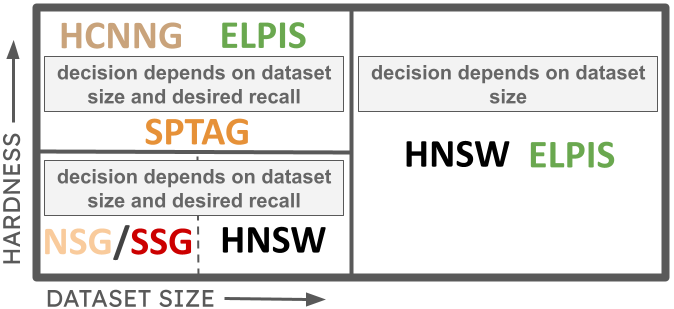
\includegraphics[width=0.6\columnwidth]{img/Experiments/recgann.png}
	 \caption{Recommendations (Indexing + 10K queries} 
    \label{fig:recgann}
	
\end{figure}

\section{Conclusion}
In this chapter, we presented ELPIS, our new approach for vector search that exploits both Graph and tree structure to leverage the power of both families of structures for efficient indexing and search performance. We have compared empirically ELPIS with twelve state-of-the-art methods for graph-based vector search, and discussed how the performance of many approaches can degrade on large size data where few succeed to scale. We also discussed the basic incremental insertion graph performance under different key components for seed selection and neighborhood diversification.
In the next section, we will present a new method for graph-based similarity search, that improves the efficiency of the search and indexing, based on the insights we have from our experimental study.
